% Options for packages loaded elsewhere
\PassOptionsToPackage{unicode}{hyperref}
\PassOptionsToPackage{hyphens}{url}
\PassOptionsToPackage{dvipsnames,svgnames*,x11names*}{xcolor}
%
\documentclass[
]{book}
\usepackage{lmodern}
\usepackage{amssymb,amsmath}
\usepackage{ifxetex,ifluatex}
\ifnum 0\ifxetex 1\fi\ifluatex 1\fi=0 % if pdftex
  \usepackage[T1]{fontenc}
  \usepackage[utf8]{inputenc}
  \usepackage{textcomp} % provide euro and other symbols
\else % if luatex or xetex
  \usepackage{unicode-math}
  \defaultfontfeatures{Scale=MatchLowercase}
  \defaultfontfeatures[\rmfamily]{Ligatures=TeX,Scale=1}
\fi
% Use upquote if available, for straight quotes in verbatim environments
\IfFileExists{upquote.sty}{\usepackage{upquote}}{}
\IfFileExists{microtype.sty}{% use microtype if available
  \usepackage[]{microtype}
  \UseMicrotypeSet[protrusion]{basicmath} % disable protrusion for tt fonts
}{}
\makeatletter
\@ifundefined{KOMAClassName}{% if non-KOMA class
  \IfFileExists{parskip.sty}{%
    \usepackage{parskip}
  }{% else
    \setlength{\parindent}{0pt}
    \setlength{\parskip}{6pt plus 2pt minus 1pt}}
}{% if KOMA class
  \KOMAoptions{parskip=half}}
\makeatother
\usepackage{xcolor}
\IfFileExists{xurl.sty}{\usepackage{xurl}}{} % add URL line breaks if available
\IfFileExists{bookmark.sty}{\usepackage{bookmark}}{\usepackage{hyperref}}
\hypersetup{
  pdftitle={Métodos quantitativos em Psicologia com R},
  pdfauthor={Luis Anunciação (PUC-Rio), PhD},
  colorlinks=true,
  linkcolor=Maroon,
  filecolor=Maroon,
  citecolor=Blue,
  urlcolor=Blue,
  pdfcreator={LaTeX via pandoc}}
\urlstyle{same} % disable monospaced font for URLs
\usepackage{color}
\usepackage{fancyvrb}
\newcommand{\VerbBar}{|}
\newcommand{\VERB}{\Verb[commandchars=\\\{\}]}
\DefineVerbatimEnvironment{Highlighting}{Verbatim}{commandchars=\\\{\}}
% Add ',fontsize=\small' for more characters per line
\usepackage{framed}
\definecolor{shadecolor}{RGB}{248,248,248}
\newenvironment{Shaded}{\begin{snugshade}}{\end{snugshade}}
\newcommand{\AlertTok}[1]{\textcolor[rgb]{0.94,0.16,0.16}{#1}}
\newcommand{\AnnotationTok}[1]{\textcolor[rgb]{0.56,0.35,0.01}{\textbf{\textit{#1}}}}
\newcommand{\AttributeTok}[1]{\textcolor[rgb]{0.77,0.63,0.00}{#1}}
\newcommand{\BaseNTok}[1]{\textcolor[rgb]{0.00,0.00,0.81}{#1}}
\newcommand{\BuiltInTok}[1]{#1}
\newcommand{\CharTok}[1]{\textcolor[rgb]{0.31,0.60,0.02}{#1}}
\newcommand{\CommentTok}[1]{\textcolor[rgb]{0.56,0.35,0.01}{\textit{#1}}}
\newcommand{\CommentVarTok}[1]{\textcolor[rgb]{0.56,0.35,0.01}{\textbf{\textit{#1}}}}
\newcommand{\ConstantTok}[1]{\textcolor[rgb]{0.00,0.00,0.00}{#1}}
\newcommand{\ControlFlowTok}[1]{\textcolor[rgb]{0.13,0.29,0.53}{\textbf{#1}}}
\newcommand{\DataTypeTok}[1]{\textcolor[rgb]{0.13,0.29,0.53}{#1}}
\newcommand{\DecValTok}[1]{\textcolor[rgb]{0.00,0.00,0.81}{#1}}
\newcommand{\DocumentationTok}[1]{\textcolor[rgb]{0.56,0.35,0.01}{\textbf{\textit{#1}}}}
\newcommand{\ErrorTok}[1]{\textcolor[rgb]{0.64,0.00,0.00}{\textbf{#1}}}
\newcommand{\ExtensionTok}[1]{#1}
\newcommand{\FloatTok}[1]{\textcolor[rgb]{0.00,0.00,0.81}{#1}}
\newcommand{\FunctionTok}[1]{\textcolor[rgb]{0.00,0.00,0.00}{#1}}
\newcommand{\ImportTok}[1]{#1}
\newcommand{\InformationTok}[1]{\textcolor[rgb]{0.56,0.35,0.01}{\textbf{\textit{#1}}}}
\newcommand{\KeywordTok}[1]{\textcolor[rgb]{0.13,0.29,0.53}{\textbf{#1}}}
\newcommand{\NormalTok}[1]{#1}
\newcommand{\OperatorTok}[1]{\textcolor[rgb]{0.81,0.36,0.00}{\textbf{#1}}}
\newcommand{\OtherTok}[1]{\textcolor[rgb]{0.56,0.35,0.01}{#1}}
\newcommand{\PreprocessorTok}[1]{\textcolor[rgb]{0.56,0.35,0.01}{\textit{#1}}}
\newcommand{\RegionMarkerTok}[1]{#1}
\newcommand{\SpecialCharTok}[1]{\textcolor[rgb]{0.00,0.00,0.00}{#1}}
\newcommand{\SpecialStringTok}[1]{\textcolor[rgb]{0.31,0.60,0.02}{#1}}
\newcommand{\StringTok}[1]{\textcolor[rgb]{0.31,0.60,0.02}{#1}}
\newcommand{\VariableTok}[1]{\textcolor[rgb]{0.00,0.00,0.00}{#1}}
\newcommand{\VerbatimStringTok}[1]{\textcolor[rgb]{0.31,0.60,0.02}{#1}}
\newcommand{\WarningTok}[1]{\textcolor[rgb]{0.56,0.35,0.01}{\textbf{\textit{#1}}}}
\usepackage{longtable,booktabs}
% Correct order of tables after \paragraph or \subparagraph
\usepackage{etoolbox}
\makeatletter
\patchcmd\longtable{\par}{\if@noskipsec\mbox{}\fi\par}{}{}
\makeatother
% Allow footnotes in longtable head/foot
\IfFileExists{footnotehyper.sty}{\usepackage{footnotehyper}}{\usepackage{footnote}}
\makesavenoteenv{longtable}
\usepackage{graphicx,grffile}
\makeatletter
\def\maxwidth{\ifdim\Gin@nat@width>\linewidth\linewidth\else\Gin@nat@width\fi}
\def\maxheight{\ifdim\Gin@nat@height>\textheight\textheight\else\Gin@nat@height\fi}
\makeatother
% Scale images if necessary, so that they will not overflow the page
% margins by default, and it is still possible to overwrite the defaults
% using explicit options in \includegraphics[width, height, ...]{}
\setkeys{Gin}{width=\maxwidth,height=\maxheight,keepaspectratio}
% Set default figure placement to htbp
\makeatletter
\def\fps@figure{htbp}
\makeatother
\setlength{\emergencystretch}{3em} % prevent overfull lines
\providecommand{\tightlist}{%
  \setlength{\itemsep}{0pt}\setlength{\parskip}{0pt}}
\setcounter{secnumdepth}{5}
\usepackage{booktabs}
\usepackage{amsthm}
\makeatletter
\def\thm@space@setup{%
  \thm@preskip=8pt plus 2pt minus 4pt
  \thm@postskip=\thm@preskip
}
\makeatother
\usepackage[]{natbib}
\bibliographystyle{apalike}

\title{Métodos quantitativos em Psicologia com R}
\author{\href{mailto:\%20luisfca@gmail.com}{Luis Anunciação (PUC-Rio), PhD}}
\date{2020-06-06}

\begin{document}
\maketitle

{
\hypersetup{linkcolor=}
\setcounter{tocdepth}{1}
\tableofcontents
}
\begin{Shaded}
\begin{Highlighting}[]
\NormalTok{knitr}\OperatorTok{::}\NormalTok{opts_chunk}\OperatorTok{$}\KeywordTok{set}\NormalTok{(}\DataTypeTok{echo =} \OtherTok{TRUE}\NormalTok{, }\DataTypeTok{fig.align=}\StringTok{"center"}\NormalTok{)}
\end{Highlighting}
\end{Shaded}

\hypertarget{introduuxe7uxe3o}{%
\chapter{Introdução}\label{introduuxe7uxe3o}}

Aprender estatística e análise de dados é uma das tarefas mais importantes e desafiadoras que existe no meio acadêmico, especialmente às disciplinas agrupadas em ciências humanas, como Psicologia. Por consequência, ensinar ambas as matérias também impõe um desafio enorme, mas necessário.

Por diversas razões, as pesquisas feitas em Psicologia apresentam muitas informações misturadas e sobrepostas e a utilização da estatística é fundamental para conseguir separar e filtrar àquelas informações que temos interesse (sinal) daquelas que apenas distorcem estas primeiras (ruído).

\hypertarget{objetivo}{%
\section{Objetivo}\label{objetivo}}

Este livro tem como objetivo introduzir conceitos teóricos e aspectos computacionais de estatística de maneira pragmática, direta ao ponto e a partir de perguntas previamente exploradas em pesquisas científicas publicadas. Em menor nível, a modelagem matemática será apresentada e descrita.

Uma das coisas mais importantes para se ter em mente neste livro é que apesar de todo conteúdo ter uma estrutura linear, os capítulos foram construídos de maneira a serem completos em si mesmo e responderem questões específicas, particulares e pontuais. Assim, penso que o livro atende tanto aqueles leitores com interesse em ler a obra inteira, como aqueles que buscam apenas informações mais específicas de um tópico particular.

Evidentemente, esse formato adotado pode gerar uma percepção diferente entre aqueles que consultarem apenas um capítulo ou outro e aqueles que lerem o conteúdo por completo. Isso ocorre pois como muitos testes estatísticos são entendidos como casos particulares de outros, alguns fragmentos que podem parecer destoantes durante uma leitura inicial em alguns capítulos, tornam-se mais fáceis e articulados àqueles que lerem o trabalho inteiro e se dispuserem a fazer uma releitura de partes específicas.

Para ilustrar, o capítulo sobre o Teste T expõe uma pequena parte sobre modelos de regressão, conteúdo que somente é abordado posteriormente. Se em um primeiro momento isso provavelmente pode gerar alguma (pequena) confusão, a releitura do capítulo após o término da sequência do livro tende a gerar, além de um conhecimento mais profundo por parte do leitor, a percepção da integração tanto da estrutura do livro, como da relação existente entre diferentes modelos estatísticos.

\hypertarget{bases}{%
\section{Bases}\label{bases}}

Todas as bases de dados utilizadas neste livro são frutos de pesquisas empíricas que apresentam artigos publicados. Uma vez que o objetivo de um livro é diferente do objetivo da publicação de um artigo, alguns ajustes foram feitos às bases para torná-las mais acessíveis. Nenhuma alteração foi realizada nos dados, mas apenas em mudanças em relação a nomes de variáveis e quantidade de vetores.

Todo material pode ser acessado livre e grauitamente em \url{https://github.com/anovabr/mqt/tree/master/bases}

\hypertarget{pacotes-e-sintaxes}{%
\section{Pacotes e sintaxes}\label{pacotes-e-sintaxes}}

Este livro utiliza majoritariamente o ambiente \href{https://www.tidyverse.org/}{tidyverse} para realização das análises. Entretanto, sempre que necessário, funções R-base e uso de outros pacotes serão utilizados. Toda codificação utilizada no livro é exibida nos capítulos e integralmente disponível gratuitamente neste (GitHub){[}\url{https://github.com/anovabr/mqt}{]}

\hypertarget{aspectos-gerais}{%
\chapter{Aspectos gerais}\label{aspectos-gerais}}

{[}Versão de testes{]} Conforme já explicitado, a estatística pode ser dividida em duas áreas interligadas: estatística descritiva e estatística inferencial. O objetivo da estatística descritiva é apresentar sínteses e resumos dos resultados a partir de gráficos e tabelas. Não é intenção dessa área fazer generalizações ou extrapolar os resultados obtidos em uma pesquisa a pessoas não investigadas durante a coleta de dados. Por contraste, a estatística inferencial visa extrapolar os dados e fazer generalizações que toquem toda população de onde aquela mostra foi retirada e é representativa. Dessa maneira, o principal objetivo da estatística inferencial é, de fato, fazer inferências.

Apesar de livros e aulas unirem ambas as áreas da estatística, alguns pontos merecem destaque, que são:

\begin{enumerate}
\def\labelenumi{\arabic{enumi}.}
\item
  A estatística descritiva surgiu antes que a inferencial. A etimologia da palavra talvez ajude a entender, uma vez que estatística vem da palavra estado e este sempre teve interesse em saber quantos eram os cidadãos de um determinado local para, entre outras atividades, taxá-los. Dessa maneira, aspectos descritivos antecedem os inferenciais. Por sua vez, a estatística inferencial guarda origem e proximidade com a teoria dos jogos e, consequentemente, isso ajuda a entender o motivo pelo qual a maioria dos exemplos inferenciais envolvem jogos de azar.
\item
  A estatística tem duas ``escolas'' ou ``formas de pensamento''. A estatística frequentista e a estatística bayesiana. Aspectos fundamentais que tocam à definição de probabilidade são diferentes, bem como a definição de dados e parâmetros também o são. Pela perspectiva histórica, a estatística bayesiana é mais antiga que a frequentista. No entanto, se for comparado a proporção de uso entre os pesquisadores, a estatística frequentista é ainda a mais frequente e justifica a ênfase deste livro nesta área.
\item
  A relação entre estatística e Machine Learning (ML) é relativamente recente. Apesar de grande interface, e do fato que as análises realizadas em estatística e ML encontram resultados virtualmente idênticos, as áreas têm objetivos diferentes. Ainda sob perspectiva histórica, a estatística, como uma área do conhecimento, é anterior à ML e, também por isso, justifica a ênfase do livro.
\end{enumerate}

\hypertarget{estatuxedstica-descritiva}{%
\chapter{Estatística Descritiva}\label{estatuxedstica-descritiva}}

\begin{objectives}
\textbf{Objetivos do capítulo}\\
1. Apresentar tabelas e gráficos\\
2. Introduzir os verbos do dplyr e funções do ggplot.\\
3. Oferecer convenções ou regras gerais para criação de gráficos
\end{objectives}

\hypertarget{pesquisa}{%
\section{Pesquisa}\label{pesquisa}}

\begin{alert}

Base: Dados - Brasil e espanha fusionados

\end{alert}

Neste capítulo (e em alguns outros), vamos utilizar a pesquisa intitulada ``Sintomas de depressão e ansiedade em universitários espanhóis, portugueses e brasileiros'', com previsão de publicação pela Revista Psicologia: Teoria e Pesquisa em 2020. Nessa pesquisa, sou o coautor e o pesquisador responsável para correspondência.

O objetivo da pesquisa foi explorar sintomas de ansiedade e depressão em universitários, bem como investigar possíveis relações entre tais traços latentes e fatores sociodemográficos. Um diferencial importante do trabalho foi a seleção amostral. Partiu-se de uma amostra estratificada (probabilística) dos estudantes de três universidades, PUC-Rio (Brasil), Universidade de Extremadura (Espanha) e Universidade de Coimbra (Portugal). Isso permitiu ter maior validade externa dos resultados.

\hypertarget{condiuxe7uxf5es-gerais}{%
\section{Condições gerais}\label{condiuxe7uxf5es-gerais}}

Todo documento acadêmico e científico é composto de aspectos textuais, tabulares e gráficos que devem caminhar na mesma direção e serem sempre associados às perguntas e objetivos traçados na pesquisa. É fácil perceber, dessa maneira, que a parte principal de qualquer trabalho acadêmico não são necessariamente os aspectos estatísticos, mas sim os objetivos e as possíveis hipóteses investigadas pelos pesquisadores. A estatística, neste sentido, é uma valiosa ferramenta de trabalho (ou uma atividade de meio) para que as perguntas sejam respondidas de forma adequada e válida.

Frequentemente, as primeiras análises descritivas começam pela apresentação de tabelas e gráficos. Da mesma forma que a construção de um prédio depende que andaimes sejam colocados, um relatório técnico depende dessas condições. Ainda neste sentido, da mesma maneira que a conclusão do prédio cursa com a retirada dos andaimes, é bem possível que as versões finais de artigos científicos ou relatórios aproveitem apenas parte dos gráficos e tabelas desenvolvidos.

Dito isso, o R e seus pacotes oferecem excelentes ferramentas para aspectos descritivos. No entanto, algumas apresentações relativamente simples frequentemente trazem uma dificuldade computacional intensa, o que pode gerar alguma desvantagem na utilização do R para tais apresentações quando comparados com programas mais acessíveis, como o Excel. No entanto, apesar dessa condição, a relação entre dificuldade e complexidade favorece o R àquelas tarefas mais complicadas, como realizar análises inferenciais e psicométricas, como apresentado a seguir.

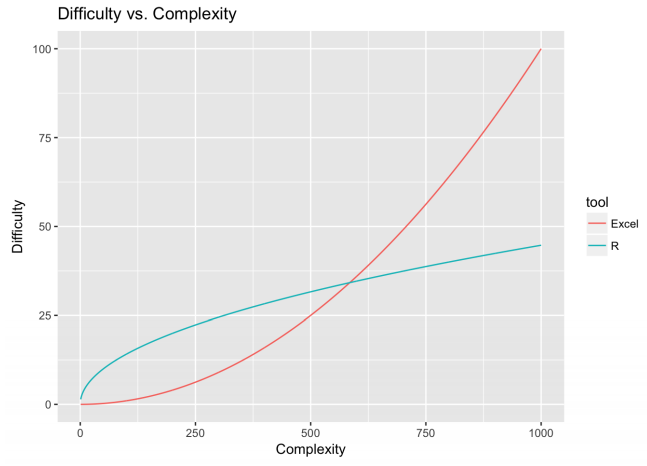
\includegraphics{./img/excel_r.PNG}

\hypertarget{verbos-do-dplyr}{%
\section{Verbos do dplyr}\label{verbos-do-dplyr}}

O dplyr funciona de maneira muito intuitiva. O padrão original do R considera que as operações são realizadas a partir de uma lógica do tipo \texttt{verbo(sujeito,\ complemento)} enquanto o ambiente tidyverse opta por \texttt{sujeito\ \%\textgreater{}\%\ verbo(complemento)}, tornando-se o ato de programar mais natural e associado à maneira que organizamos as ideias.

Os verbos principais do pacote estão listados na tabela a seguir e as sintaxes deixadas no decorrer deste capítulo (e do livro) permitem uma melhor apreensão das funcionalidades. É importante lembrar que, em alguns momentos, em função da praticidade computacional, algumas sintaxes vão contar com o formato base do R.

\begin{longtable}[]{@{}lc@{}}
\toprule
Verbo & Ação\tabularnewline
\midrule
\endhead
glimpse & Inspeciona os dados\tabularnewline
count & Conta os níveis de uma variável\tabularnewline
select & seleciona uma variável específica\tabularnewline
filter & Filtra os resultados por um nível específico de uma variável\tabularnewline
group\_by & Agrupa os resultados por níveis de uma variávei específica\tabularnewline
summarise & Apresenta sumários (com medidas estatísticas)\tabularnewline
mutate & Cria novas variáveis ou altera as existentes\tabularnewline
arrange & Organiza a apresentação dos resultados\tabularnewline
left\_join & Junta bases ou colunas\tabularnewline
pivot\_longer & Transforma uma base larga em longa\tabularnewline
pivot\_wider & Transforma uma base longa em larga\tabularnewline
\bottomrule
\end{longtable}

É também importante ficar atento às atualizações do dplyr e do sistema tidyverse como um todo. Eventualmente, mudanças podem ocorrer e impossibilitar (ou dificultar) a reprodução de rotinas antigas. O \href{https://www.tidyverse.org/}{site} é o local ideal para acompanhar as atualizações.

\hypertarget{tabelas}{%
\section{Tabelas}\label{tabelas}}

Tabelas apresentam os sumários informacionais de uma pesquisa de maneira reunida e objetiva. Como os verbos do dplyr possibilitam que os mesmos resultados sejam encontrados por vias diferentes, os códigos a seguir tentarão manter uma uniformidade lógica. Em alguns momentos, para ampliar as possibilidades de codificação, sintaxes extras serão oferecidas.

A tabela a seguir apresenta a quantidade de participantes em cada país.

\begin{Shaded}
\begin{Highlighting}[]
\NormalTok{Dataset }\OperatorTok\StringTok{ }
\StringTok{  }\KeywordTok{group_by}\NormalTok{(country) }\OperatorTok\StringTok{ }
\StringTok{  }\KeywordTok{summarise}\NormalTok{(}\DataTypeTok{n=}\KeywordTok{n}\NormalTok{()) }\OperatorTok\StringTok{ }
\StringTok{  }\KeywordTok{kable}\NormalTok{(}\DataTypeTok{digits =} \DecValTok{2}\NormalTok{) }\OperatorTok\StringTok{ }
\StringTok{  }\KeywordTok{kable_styling}\NormalTok{(}\DataTypeTok{bootstrap_options =} \KeywordTok{c}\NormalTok{(}\StringTok{"striped"}\NormalTok{, }\StringTok{"hover"}\NormalTok{, }\StringTok{"condensed"}\NormalTok{))}
\end{Highlighting}
\end{Shaded}

\begin{verbatim}
## `summarise()` ungrouping output (override with `.groups` argument)
\end{verbatim}

country

n

Espanha

1216

Portugal

426

Brasil

315

É também possível adicionar proporções relativas à tabela, o que é uma escolha adequada para apresentação dos resultados.

\begin{Shaded}
\begin{Highlighting}[]
\NormalTok{Dataset }\OperatorTok\StringTok{ }
\StringTok{  }\KeywordTok{group_by}\NormalTok{(country) }\OperatorTok\StringTok{ }
\StringTok{  }\KeywordTok{summarise}\NormalTok{(}\DataTypeTok{n=}\KeywordTok{n}\NormalTok{(), }\DataTypeTok{Prop =}\NormalTok{ n}\OperatorTok{/}\KeywordTok{nrow}\NormalTok{(.)) }\OperatorTok\StringTok{ }
\StringTok{  }\KeywordTok{kable}\NormalTok{(}\DataTypeTok{digits =} \DecValTok{2}\NormalTok{) }\OperatorTok\StringTok{ }
\StringTok{  }\KeywordTok{kable_styling}\NormalTok{(}\DataTypeTok{bootstrap_options =} \KeywordTok{c}\NormalTok{(}\StringTok{"striped"}\NormalTok{, }\StringTok{"hover"}\NormalTok{, }\StringTok{"condensed"}\NormalTok{))}
\end{Highlighting}
\end{Shaded}

\begin{verbatim}
## `summarise()` ungrouping output (override with `.groups` argument)
\end{verbatim}

country

n

Prop

Espanha

1216

0.62

Portugal

426

0.22

Brasil

315

0.16

O pacote \texttt{janitor} oferece complementos úteis à família tidyverse e um deles justamente adiciona os totais, de maneira mais rápida e, em função disso, os exemplos também irão acessar as funções deste pacote.

\begin{Shaded}
\begin{Highlighting}[]
\NormalTok{Dataset }\OperatorTok\StringTok{ }
\StringTok{  }\KeywordTok{tabyl}\NormalTok{(country) }\OperatorTok\StringTok{ }
\StringTok{  }\KeywordTok{adorn_totals}\NormalTok{() }\OperatorTok\StringTok{ }
\StringTok{  }\KeywordTok{kable}\NormalTok{(}\DataTypeTok{digits =} \DecValTok{2}\NormalTok{) }\OperatorTok\StringTok{ }
\StringTok{  }\KeywordTok{kable_styling}\NormalTok{(}\DataTypeTok{bootstrap_options =} \KeywordTok{c}\NormalTok{(}\StringTok{"striped"}\NormalTok{, }\StringTok{"hover"}\NormalTok{, }\StringTok{"condensed"}\NormalTok{))}
\end{Highlighting}
\end{Shaded}

country

n

percent

Espanha

1216

0.62

Portugal

426

0.22

Brasil

315

0.16

Total

1957

1.00

O mesmo que foi realizado com os países, pode também ser realizado com o sexo do participante.

\begin{Shaded}
\begin{Highlighting}[]
\NormalTok{Dataset }\OperatorTok\StringTok{ }
\StringTok{  }\KeywordTok{tabyl}\NormalTok{(sex) }\OperatorTok\StringTok{ }
\StringTok{  }\KeywordTok{adorn_totals}\NormalTok{() }\OperatorTok\StringTok{ }
\StringTok{  }\KeywordTok{kable}\NormalTok{(}\DataTypeTok{digits =} \DecValTok{2}\NormalTok{) }\OperatorTok\StringTok{ }
\StringTok{  }\KeywordTok{kable_styling}\NormalTok{(}\DataTypeTok{bootstrap_options =} \KeywordTok{c}\NormalTok{(}\StringTok{"striped"}\NormalTok{, }\StringTok{"hover"}\NormalTok{, }\StringTok{"condensed"}\NormalTok{))}
\end{Highlighting}
\end{Shaded}

sex

n

percent

valid\_percent

M

736

0.38

0.38

F

1214

0.62

0.62

NA

7

0.00

NA

Total

1957

1.00

1.00

A adição do argumento para filtrar os participantes com dados ausentes sobre sexo auxilia a apresentar melhor os resultados. É importante atentar que essa análise tem finalidade descritiva e que omitir a apresentação de variáveis ausentes não significa excluir ou remover os participantes das análises que serão feitas posteriormente. Somente em possibilidades remotas se retira participantes das análises de maneira definitiva.

\begin{Shaded}
\begin{Highlighting}[]
\NormalTok{Dataset }\OperatorTok\StringTok{ }
\StringTok{  }\KeywordTok{filter}\NormalTok{(}\OperatorTok{!}\KeywordTok{is.na}\NormalTok{(sex)) }\OperatorTok\StringTok{ }
\StringTok{  }\KeywordTok{tabyl}\NormalTok{(sex) }\OperatorTok\StringTok{ }
\StringTok{  }\KeywordTok{adorn_totals}\NormalTok{() }\OperatorTok\StringTok{ }
\StringTok{  }\KeywordTok{kable}\NormalTok{(}\DataTypeTok{digits =} \DecValTok{2}\NormalTok{) }\OperatorTok\StringTok{ }
\StringTok{  }\KeywordTok{kable_styling}\NormalTok{(}\DataTypeTok{bootstrap_options =} \KeywordTok{c}\NormalTok{(}\StringTok{"striped"}\NormalTok{, }\StringTok{"hover"}\NormalTok{, }\StringTok{"condensed"}\NormalTok{))}
\end{Highlighting}
\end{Shaded}

sex

n

percent

M

736

0.38

F

1214

0.62

Total

1950

1.00

Para fazer uma tabela cruzada, em que seja possível apresentar a quantidade de homens e mulheres por país, épossível utilizar função \texttt{pivot\_wider}:

\begin{Shaded}
\begin{Highlighting}[]
\NormalTok{Dataset }\OperatorTok\StringTok{ }
\StringTok{  }\KeywordTok{filter}\NormalTok{(}\OperatorTok{!}\KeywordTok{is.na}\NormalTok{(sex)) }\OperatorTok\StringTok{ }
\StringTok{  }\KeywordTok{count}\NormalTok{(country,sex) }\OperatorTok\StringTok{ }
\StringTok{  }\KeywordTok{pivot_wider}\NormalTok{(}\DataTypeTok{names_from =}\NormalTok{ sex, }\DataTypeTok{values_from =}\NormalTok{ n) }\OperatorTok\StringTok{ }
\StringTok{  }\KeywordTok{kable}\NormalTok{(}\DataTypeTok{digits =} \DecValTok{2}\NormalTok{) }\OperatorTok\StringTok{ }
\StringTok{  }\KeywordTok{kable_styling}\NormalTok{(}\DataTypeTok{bootstrap_options =} \KeywordTok{c}\NormalTok{(}\StringTok{"striped"}\NormalTok{, }\StringTok{"hover"}\NormalTok{, }\StringTok{"condensed"}\NormalTok{))}
\end{Highlighting}
\end{Shaded}

country

M

F

Espanha

384

825

Portugal

203

223

Brasil

149

166

Da mesma maneira como continuar com o \texttt{tabyl}, mas agora adicionando uma variável.

\begin{Shaded}
\begin{Highlighting}[]
\NormalTok{Dataset }\OperatorTok\StringTok{ }
\StringTok{  }\KeywordTok{filter}\NormalTok{(}\OperatorTok{!}\KeywordTok{is.na}\NormalTok{(sex)) }\OperatorTok\StringTok{ }
\StringTok{  }\KeywordTok{tabyl}\NormalTok{(country, sex) }\OperatorTok\StringTok{ }
\StringTok{  }\KeywordTok{adorn_totals}\NormalTok{() }\OperatorTok\StringTok{ }
\StringTok{  }\KeywordTok{kable}\NormalTok{(}\DataTypeTok{digits =} \DecValTok{2}\NormalTok{) }\OperatorTok\StringTok{ }
\StringTok{  }\KeywordTok{kable_styling}\NormalTok{(}\DataTypeTok{bootstrap_options =} \KeywordTok{c}\NormalTok{(}\StringTok{"striped"}\NormalTok{, }\StringTok{"hover"}\NormalTok{, }\StringTok{"condensed"}\NormalTok{))}
\end{Highlighting}
\end{Shaded}

country

M

F

Espanha

384

825

Portugal

203

223

Brasil

149

166

Total

736

1214

Finalmente, para apresentar a quantidade de participantes totais, bem como separar a quantidade e a porcentagem de homens e mulheres por país, a codificação torna-se mais densa. O código abaixo apresenta os comentários para auxiliar no entendimento da rotina.

\begin{Shaded}
\begin{Highlighting}[]
\NormalTok{Dataset }\OperatorTok\StringTok{ }\CommentTok{#get data}
\StringTok{  }\CommentTok{#filter }
\StringTok{  }\KeywordTok{filter}\NormalTok{(}\OperatorTok{!}\KeywordTok{is.na}\NormalTok{(sex)) }\OperatorTok\StringTok{ }
\StringTok{  }
\StringTok{  }\CommentTok{#agrupar}
\StringTok{  }\KeywordTok{group_by}\NormalTok{(country, }\DataTypeTok{add=}\OtherTok{TRUE}\NormalTok{) }\OperatorTok\StringTok{ }
\StringTok{  }\KeywordTok{mutate}\NormalTok{(}\DataTypeTok{participantes =} \KeywordTok{n}\NormalTok{()) }\OperatorTok\StringTok{ }

\StringTok{  }\CommentTok{#adicionar a relacao de quantidade de pais e sexo}
\StringTok{  }\KeywordTok{group_by}\NormalTok{(country, sex, participantes, }\DataTypeTok{add=}\OtherTok{TRUE}\NormalTok{) }\OperatorTok\StringTok{ }

\StringTok{  }\KeywordTok{summarise}\NormalTok{(}
    \CommentTok{#cria a contagem de sexo}
    \DataTypeTok{sex_count =} \KeywordTok{n}\NormalTok{(), }
    \CommentTok{#cria a porcentagem de sexo por pais}
    \DataTypeTok{sex_percentage =} \KeywordTok{round}\NormalTok{(sex_count}\OperatorTok{/}\KeywordTok{first}\NormalTok{(participantes),}\DecValTok{2}\NormalTok{)) }\OperatorTok
\StringTok{  }\CommentTok{# cria uma variável agrupada}
\StringTok{    }\KeywordTok{mutate}\NormalTok{(}\DataTypeTok{n_percentage =} \KeywordTok{paste0}\NormalTok{(sex_count,}\StringTok{" ("}\NormalTok{,sex_percentage,}\StringTok{")"}\NormalTok{)) }\OperatorTok\StringTok{ }
\StringTok{  }\CommentTok{#seleciona apenas as variaveis de interesse}
\StringTok{  }\KeywordTok{select}\NormalTok{(country, sex, n_percentage, participantes)  }\OperatorTok
\StringTok{  }\CommentTok{#Muda para formato largo de apresentação}
\StringTok{    }\KeywordTok{spread}\NormalTok{(sex, n_percentage, }\DataTypeTok{fill=}\StringTok{"-"}\NormalTok{) }\OperatorTok\StringTok{ }
\StringTok{  }\CommentTok{#coloca os totais}
\StringTok{  }\NormalTok{janitor}\OperatorTok{::}\KeywordTok{adorn_totals}\NormalTok{(}\StringTok{"row"}\NormalTok{) }\OperatorTok\StringTok{ }
\StringTok{  }\KeywordTok{kable}\NormalTok{(., }\DataTypeTok{digits =} \DecValTok{2}\NormalTok{,  }\DataTypeTok{booktabs =}\NormalTok{ T) }\OperatorTok
\StringTok{  }\KeywordTok{kable_styling}\NormalTok{(}\DataTypeTok{position =} \StringTok{"center"}\NormalTok{, }\DataTypeTok{full_width =}\NormalTok{ F, }\DataTypeTok{bootstrap_options =} \StringTok{"striped"}\NormalTok{)}
\end{Highlighting}
\end{Shaded}

\begin{verbatim}
## `summarise()` regrouping output by 'country', 'sex' (override with `.groups` argument)
\end{verbatim}

country

participantes

M

F

Espanha

1209

384 (0.32)

825 (0.68)

Portugal

426

203 (0.48)

223 (0.52)

Brasil

315

149 (0.47)

166 (0.53)

Total

1950

\begin{itemize}
\item
  \begin{itemize}
  \item
  \end{itemize}
\end{itemize}

Ainda a partir da função \texttt{tabyl}, a realização desta tabela é simplificada.

\begin{Shaded}
\begin{Highlighting}[]
\NormalTok{Dataset }\OperatorTok
\StringTok{  }\KeywordTok{filter}\NormalTok{(}\OperatorTok{!}\KeywordTok{is.na}\NormalTok{(sex)) }\OperatorTok\StringTok{ }
\StringTok{  }\KeywordTok{tabyl}\NormalTok{(country, sex) }\OperatorTok
\StringTok{  }\KeywordTok{adorn_totals}\NormalTok{(}\KeywordTok{c}\NormalTok{(}\StringTok{"row"}\NormalTok{, }\StringTok{"col"}\NormalTok{)) }\OperatorTok
\StringTok{  }\KeywordTok{adorn_percentages}\NormalTok{(}\StringTok{"row"}\NormalTok{) }\OperatorTok\StringTok{ }
\StringTok{  }\KeywordTok{adorn_pct_formatting}\NormalTok{(}\DataTypeTok{rounding =} \StringTok{"half up"}\NormalTok{, }\DataTypeTok{digits =} \DecValTok{0}\NormalTok{) }\OperatorTok
\StringTok{  }\KeywordTok{adorn_ns}\NormalTok{() }\OperatorTok
\StringTok{  }\KeywordTok{adorn_title}\NormalTok{(}\StringTok{"combined"}\NormalTok{) }\OperatorTok
\StringTok{  }\KeywordTok{kable}\NormalTok{(., }\DataTypeTok{digits =} \DecValTok{2}\NormalTok{,  }\DataTypeTok{booktabs =}\NormalTok{ T) }\OperatorTok
\StringTok{  }\KeywordTok{kable_styling}\NormalTok{(}\DataTypeTok{position =} \StringTok{"center"}\NormalTok{, }\DataTypeTok{full_width =}\NormalTok{ F, }\DataTypeTok{bootstrap_options =} \StringTok{"striped"}\NormalTok{)}
\end{Highlighting}
\end{Shaded}

country/sex

M

F

Total

Espanha

32\% (384)

68\% (825)

100\% (1209)

Portugal

48\% (203)

52\% (223)

100\% (426)

Brasil

47\% (149)

53\% (166)

100\% (315)

Total

38\% (736)

62\% (1214)

100\% (1950)

\hypertarget{gruxe1ficos}{%
\section{Gráficos}\label{gruxe1ficos}}

A máquina gráfica do tidyverse é o ggplot. Pelo menos 3 argumentos são necessários para criação de gráficos, que são:

\begin{enumerate}
\def\labelenumi{\arabic{enumi}.}
\tightlist
\item
  O banco dados \texttt{(data\ =\ )}, que pode ser omitido da sintaxe,\\
\item
  O aspecto estético, que permite diferentes complementos \texttt{aes(x\ =\ ,\ y\ =\ ,\ fill\ =\ ,\ color\ =\ )},\\
\item
  O aspecto geométrico, que varia em função do gráfico a ser apresentado \texttt{geom\_}
\end{enumerate}

É também possível adicionar outros argumentos, como:\\
4. Transformações estatísticas \texttt{stat\_summary}\\
5. Facetas para dividir a visualização \texttt{facet\_}\\
6. Sistema de coordenadas \texttt{coord\_}\\
7. Temas específicos \texttt{theme\_}

É importante notar que apesar dos argumentos utilizados na sintaxe serem similares aos utilizados em toda família tidyverse, a ligação \texttt{\%\textgreater{}\%} é substituída pelo \texttt{+}.

Quando bem feitos, os gráficos são extremamente úteis. Como aponta Morettin e Bussab \citep{morettin_bussab_2010}, eles possibilitam:\\
(a) buscar padrões e relações;\\
(b) confirmar (ou não) certas expectativas que se tinha sobre os dados;\\
(c) descobrir novos fenômenos;\\
(d) confirmar (ou não) suposições feitas sobre os procedimentos estatísticos usados; e\\
(e) apresentar resultados de modo mais rápido e fácil.

É sempre bom que o gráfico tenha um título e uma escala. A maioria dos gráficos são apresentados em um plano com um eixo horizontal (abcissas) e um vertical (ordenadas). Por sua vez, tais planos se referem, nessa ordem, ou aos níveis da variável que está sendo medida (eixo x) e as contagens ou proporções encontradas (eixo y) ou aos níveis da variável independente (eixo x) e os resultados médios da variável dependente (eixo y).

Para eleger que gráfico será realizado, é necessário responder a duas perguntas que são atreladas às pesquisas em Psicologia e áreas congêneres:\\
1. Quantas variáveis serão apresentadas ?\\
2. Qual o nível de medida da variával independente ?

O diagrama abaixo oferece uma árvore de decisão funcional.

\begin{verbatim}
## PhantomJS not found. You can install it with webshot::install_phantomjs(). If it is installed, please make sure the phantomjs executable can be found via the PATH variable.
\end{verbatim}

\hypertarget{htmlwidget-8765dcbeed66bacca0a7}{}
\begin{grViz}

\end{grViz}

\hypertarget{variuxe1vel-discreta}{%
\section{1 variável discreta}\label{variuxe1vel-discreta}}

Quando há apenas uma variável discreta (incluindo aqui as categóricas), os gráficos são criados para apresentar as contagens e/ou suas proporções. Nesse caso, é recomendado utilização de um gráfico de barras ou gráfico de setor. Apesar de ser possível apresentar as frequências absolutas, esses resultados podem gerar distorção da informação e, portanto, é preferível sempre apresentar as proporções de ocorrência de uma determinada variável ou valor. Por definição, quando se trabalha com proporções, o valor máximo da soma das proporções é 100.

O gráfico de barras abaixo apresenta a contagem absoluta dos participantes pesquisados em cada país.

\begin{Shaded}
\begin{Highlighting}[]
\KeywordTok{ggplot}\NormalTok{(Dataset, }\KeywordTok{aes}\NormalTok{(}\DataTypeTok{x =}\NormalTok{ country)) }\OperatorTok{+}
\StringTok{  }\KeywordTok{geom_bar}\NormalTok{(}\DataTypeTok{stats =}\NormalTok{ identity) }\OperatorTok{+}
\StringTok{  }\KeywordTok{labs}\NormalTok{(}\DataTypeTok{x =} \StringTok{"País"}\NormalTok{, }\DataTypeTok{title =} \StringTok{"Número de participantes nos países investigados"}\NormalTok{)}
\end{Highlighting}
\end{Shaded}

\begin{verbatim}
## Warning: Ignoring unknown parameters: stats
\end{verbatim}

\begin{center}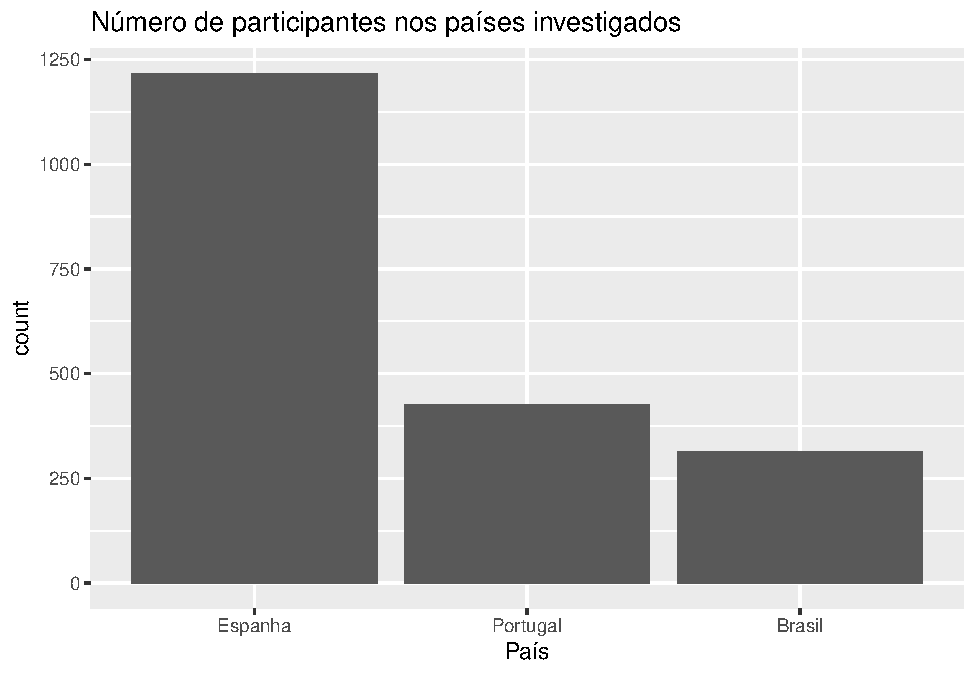
\includegraphics{gitbook-demo_files/figure-latex/unnamed-chunk-13-1} \end{center}

Já abaixo, as barras são utilizadas considerando os resultados proporcionais. Para isso, um recurso do pacote \texttt{scales} foi utilizado para adequar o eixo y e também para adicionar o valor às colunas.

\begin{Shaded}
\begin{Highlighting}[]
\KeywordTok{ggplot}\NormalTok{(Dataset, }\KeywordTok{aes}\NormalTok{(}\DataTypeTok{x =}\NormalTok{ country, }\DataTypeTok{y =}\NormalTok{ ..prop.., }\DataTypeTok{group =} \DecValTok{1}\NormalTok{)) }\OperatorTok{+}\StringTok{ }
\StringTok{  }\KeywordTok{geom_bar}\NormalTok{(}\DataTypeTok{stat =} \StringTok{"count"}\NormalTok{) }\OperatorTok{+}
\StringTok{  }\KeywordTok{geom_text}\NormalTok{(}\KeywordTok{aes}\NormalTok{(}\DataTypeTok{label=}\NormalTok{scales}\OperatorTok{::}\KeywordTok{percent}\NormalTok{(}\KeywordTok{round}\NormalTok{(..prop..,}\DecValTok{2}\NormalTok{)), }
                \DataTypeTok{y=}\NormalTok{..prop..), }\DataTypeTok{stat=} \StringTok{"count"}\NormalTok{, }\DataTypeTok{color =} \StringTok{"white"}\NormalTok{, }\DataTypeTok{size =} \DecValTok{3}\NormalTok{, }\DataTypeTok{position =} \KeywordTok{position_stack}\NormalTok{(}\DataTypeTok{vjust =} \FloatTok{0.5}\NormalTok{)) }\OperatorTok{+}
\StringTok{  }\KeywordTok{scale_y_continuous}\NormalTok{(}\DataTypeTok{labels =}\NormalTok{ scales}\OperatorTok{::}\KeywordTok{percent_format}\NormalTok{()) }\OperatorTok{+}
\StringTok{  }\KeywordTok{labs}\NormalTok{(}\DataTypeTok{x =} \StringTok{"País"}\NormalTok{, }\DataTypeTok{title =} \StringTok{"Proporção de participantes em cada país investigado"}\NormalTok{)}
\end{Highlighting}
\end{Shaded}

\begin{center}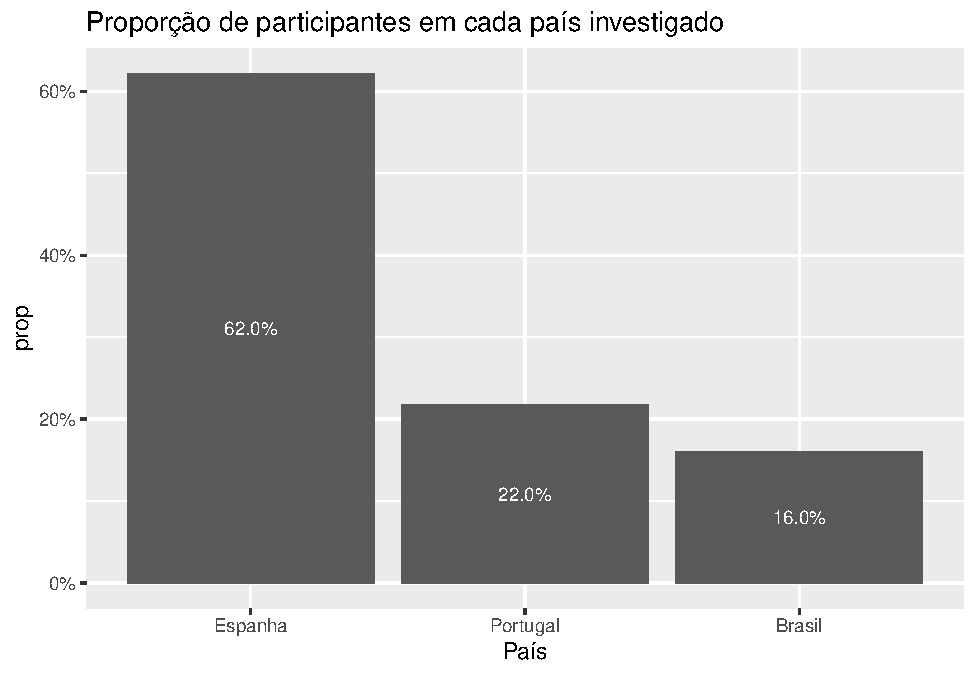
\includegraphics{gitbook-demo_files/figure-latex/unnamed-chunk-14-1} \end{center}

O gráfico de setor (as vezes chamado de pizza ou torta) pode também ser utilizado. O aspecto principal desse gráfico é apresentar os setores de maneira proporcional às frequências.

\begin{Shaded}
\begin{Highlighting}[]
\KeywordTok{ggplot}\NormalTok{(Dataset, }\KeywordTok{aes}\NormalTok{(}\DataTypeTok{x=}\KeywordTok{factor}\NormalTok{(}\DecValTok{1}\NormalTok{), }\DataTypeTok{fill=}\NormalTok{country))}\OperatorTok{+}
\StringTok{  }\KeywordTok{geom_bar}\NormalTok{(}\DataTypeTok{width =} \DecValTok{1}\NormalTok{) }\OperatorTok{+}
\StringTok{  }\KeywordTok{coord_polar}\NormalTok{(}\StringTok{"y"}\NormalTok{) }\OperatorTok{+}
\StringTok{  }\KeywordTok{labs}\NormalTok{(}\DataTypeTok{title =} \StringTok{"Proporção de participantes em cada país"}\NormalTok{)}
\end{Highlighting}
\end{Shaded}

\begin{center}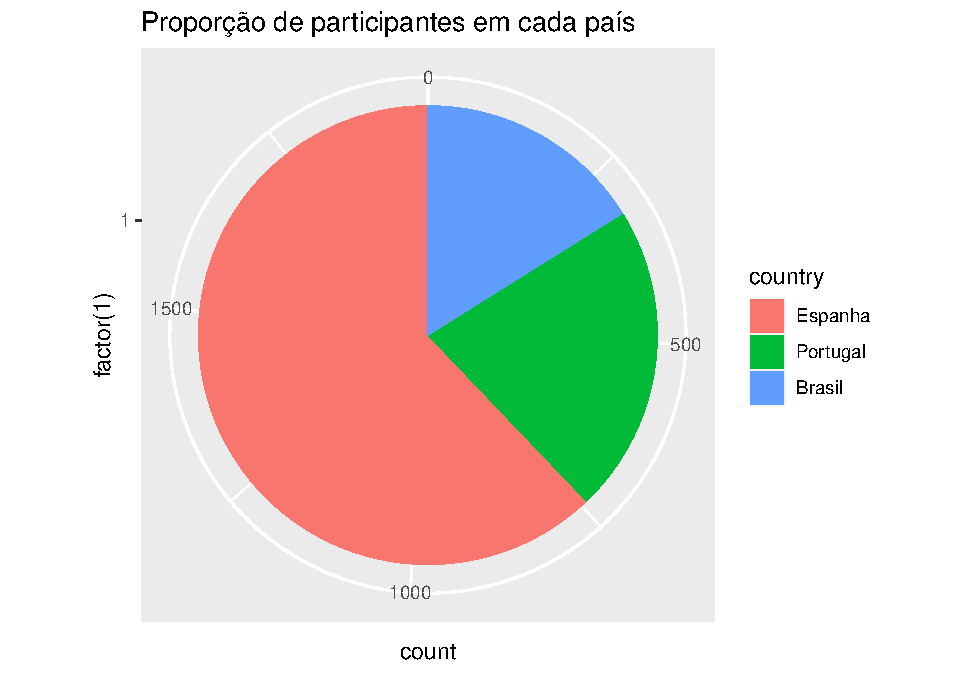
\includegraphics{gitbook-demo_files/figure-latex/unnamed-chunk-15-1} \end{center}

\hypertarget{variuxe1vel-contuxednua}{%
\section{1 variável contínua}\label{variuxe1vel-contuxednua}}

Quando uma única variável é apresentada no gráfico e ela é continua, os gráficos adequados são o histograma, densidade e o boxplot.

Abaixo um histograma da idade dos participantes:

\begin{Shaded}
\begin{Highlighting}[]
\KeywordTok{ggplot}\NormalTok{(Dataset, }\KeywordTok{aes}\NormalTok{(}\DataTypeTok{x =}\NormalTok{ age)) }\OperatorTok{+}
\StringTok{  }\KeywordTok{geom_histogram}\NormalTok{(}\DataTypeTok{bins =} \DecValTok{30}\NormalTok{, }\DataTypeTok{color =} \StringTok{"black"}\NormalTok{, }\DataTypeTok{fill =} \StringTok{"lightgrey"}\NormalTok{) }\OperatorTok{+}
\StringTok{  }\KeywordTok{labs}\NormalTok{(}\DataTypeTok{title =} \StringTok{"Distribuição da idade dos participantes"}\NormalTok{)}
\end{Highlighting}
\end{Shaded}

\begin{verbatim}
## Warning: Removed 28 rows containing non-finite values (stat_bin).
\end{verbatim}

\begin{center}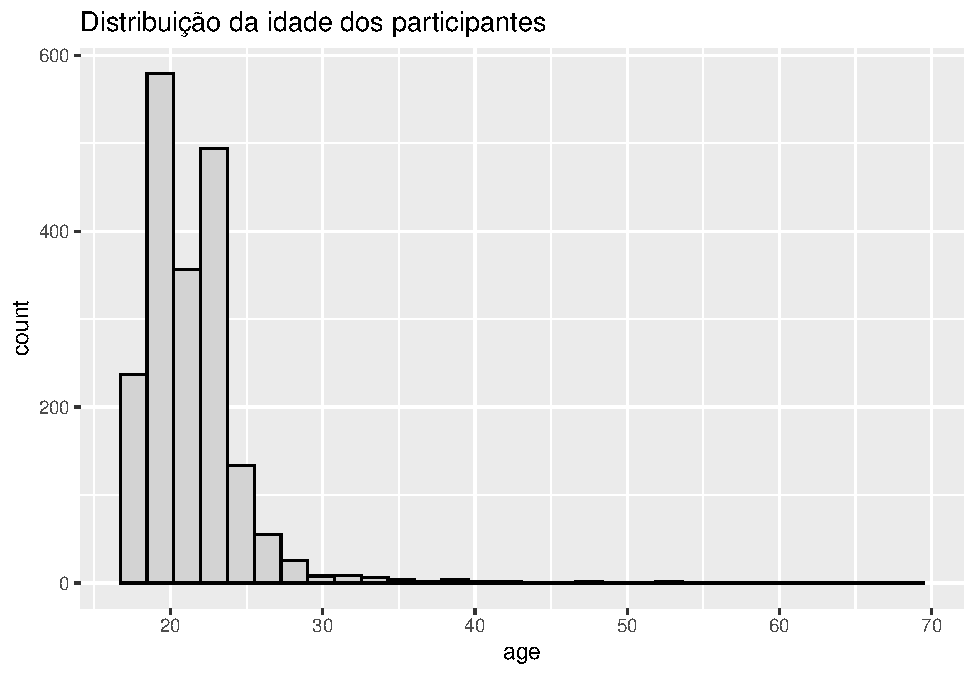
\includegraphics{gitbook-demo_files/figure-latex/unnamed-chunk-16-1} \end{center}

Abaixo um gráfico de densidade da idade:

\begin{Shaded}
\begin{Highlighting}[]
\KeywordTok{ggplot}\NormalTok{(Dataset, }\KeywordTok{aes}\NormalTok{(}\DataTypeTok{x =}\NormalTok{ age)) }\OperatorTok{+}
\StringTok{  }\KeywordTok{geom_density}\NormalTok{(}\DataTypeTok{fill =} \StringTok{"lightgray"}\NormalTok{) }\OperatorTok{+}
\StringTok{  }\KeywordTok{labs}\NormalTok{(}\DataTypeTok{title =} \StringTok{"Distribuição da idade dos participantes"}\NormalTok{)}
\end{Highlighting}
\end{Shaded}

\begin{verbatim}
## Warning: Removed 28 rows containing non-finite values (stat_density).
\end{verbatim}

\begin{center}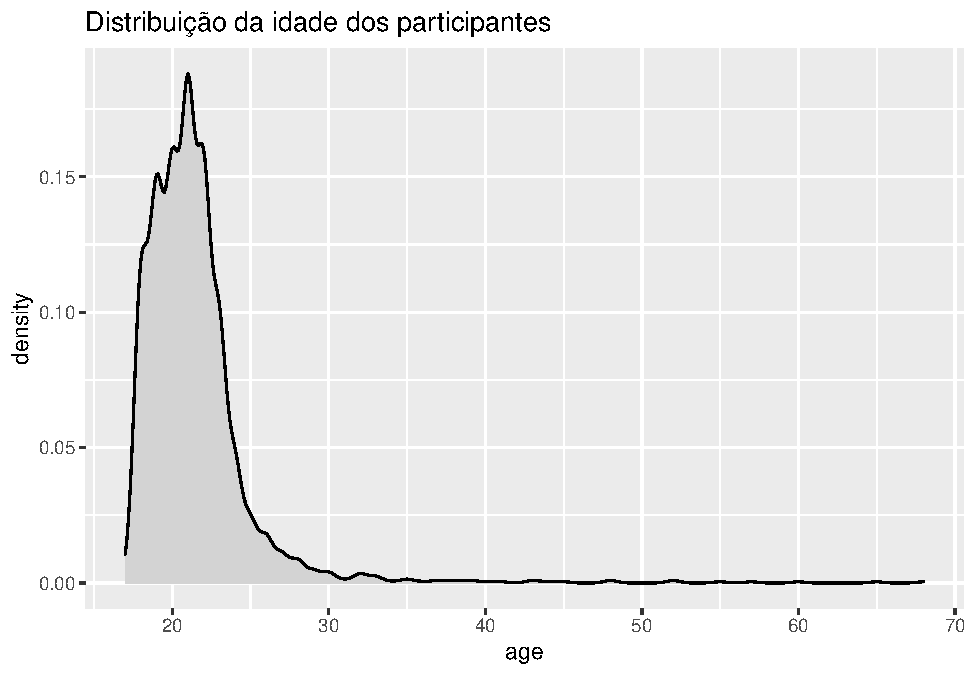
\includegraphics{gitbook-demo_files/figure-latex/unnamed-chunk-17-1} \end{center}

Por sua vez, abaixo o boxplot dessa mesma variável:

\begin{Shaded}
\begin{Highlighting}[]
\KeywordTok{ggplot}\NormalTok{(Dataset, }\KeywordTok{aes}\NormalTok{(}\DataTypeTok{y =}\NormalTok{ age, }\DataTypeTok{x =} \StringTok{""}\NormalTok{)) }\OperatorTok{+}
\StringTok{  }\KeywordTok{geom_boxplot}\NormalTok{() }\OperatorTok{+}
\StringTok{  }\KeywordTok{labs}\NormalTok{(}\DataTypeTok{title =} \StringTok{"Distribuição da idade dos participantes"}\NormalTok{)}
\end{Highlighting}
\end{Shaded}

\begin{verbatim}
## Warning: Removed 28 rows containing non-finite values (stat_boxplot).
\end{verbatim}

\begin{center}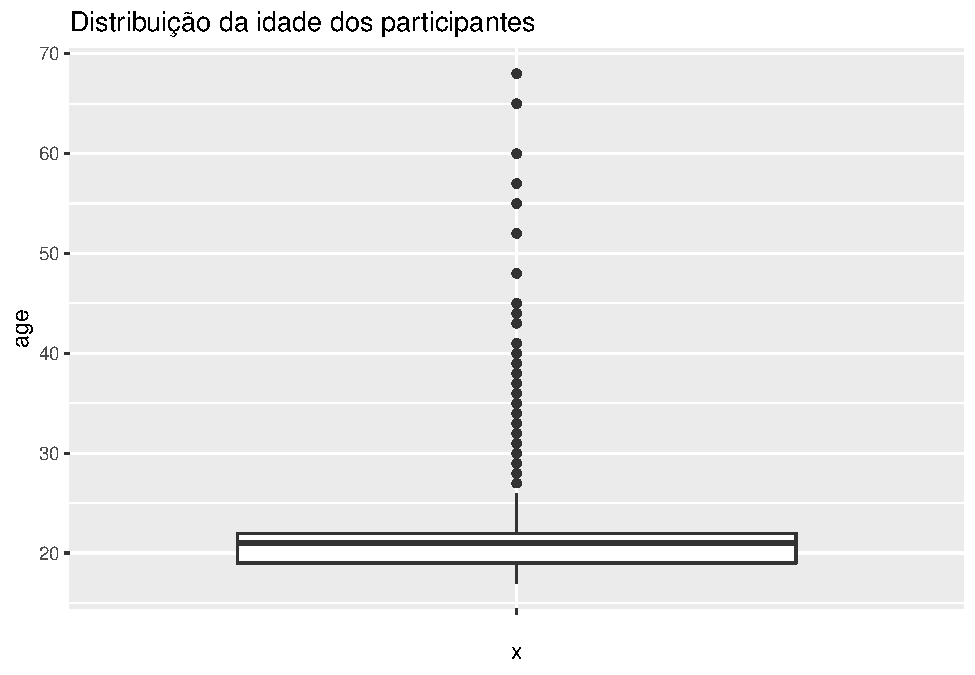
\includegraphics{gitbook-demo_files/figure-latex/unnamed-chunk-18-1} \end{center}

O boxplot tem vantagens em comparação com os outros gráficos apresentados até agora. A caixa reúne 50\% da distribuição (Q1, Mediana e Q3) e os bigodes são construídos com base em \texttt{Q1\ -\ 1.5*IQR} e \texttt{Q3\ +\ 1.5*IQR}.

Apesar de algo difícil de visualizar ao início, a informação apresentada no boxplot e no gráfico de densidade são iguais.

\begin{Shaded}
\begin{Highlighting}[]
\NormalTok{gridExtra}\OperatorTok{::}\KeywordTok{grid.arrange}\NormalTok{(}
  \CommentTok{#Grafico 1}
  \KeywordTok{ggplot}\NormalTok{(Dataset, }\KeywordTok{aes}\NormalTok{(}\DataTypeTok{x =}\NormalTok{ age)) }\OperatorTok{+}
\StringTok{  }\KeywordTok{geom_density}\NormalTok{(}\DataTypeTok{fill =} \StringTok{"lightgray"}\NormalTok{),}
  
  \CommentTok{#Grafico 2}
  \KeywordTok{ggplot}\NormalTok{(Dataset, }\KeywordTok{aes}\NormalTok{(}\DataTypeTok{y =}\NormalTok{ age, }\DataTypeTok{x =} \StringTok{""}\NormalTok{)) }\OperatorTok{+}
\StringTok{  }\KeywordTok{geom_boxplot}\NormalTok{() }\OperatorTok{+}
\StringTok{  }\KeywordTok{coord_flip}\NormalTok{(),}
  
  \DataTypeTok{top =} \StringTok{"Distribuição da idade dos participantes"} \CommentTok{#título}
\NormalTok{)}
\end{Highlighting}
\end{Shaded}

\begin{verbatim}
## Warning: Removed 28 rows containing non-finite values (stat_density).
\end{verbatim}

\begin{verbatim}
## Warning: Removed 28 rows containing non-finite values (stat_boxplot).
\end{verbatim}

\begin{center}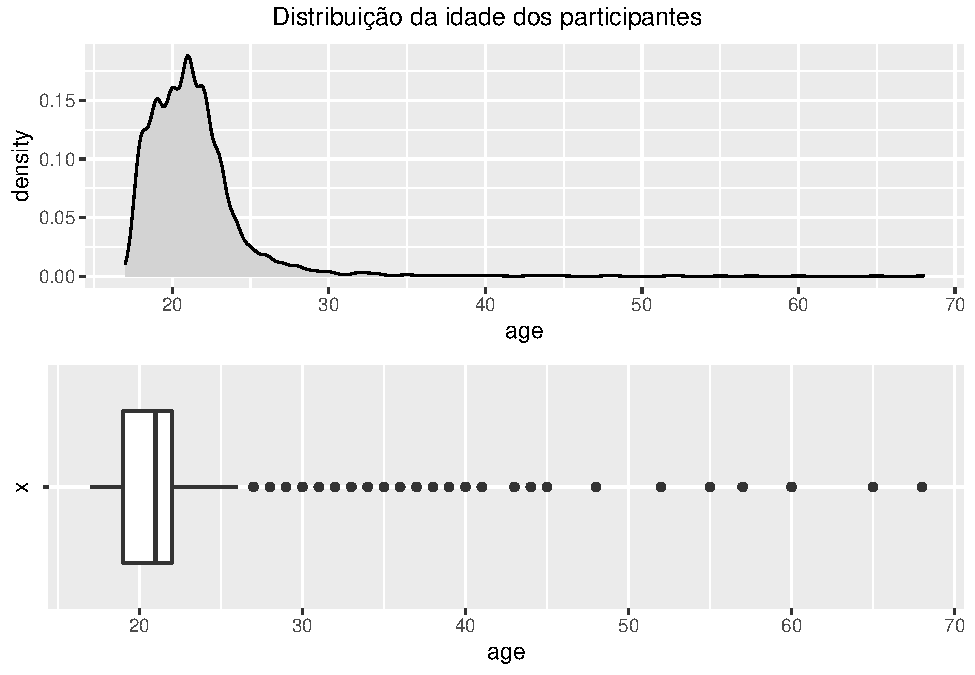
\includegraphics{gitbook-demo_files/figure-latex/unnamed-chunk-19-1} \end{center}

\hypertarget{variuxe1veis-com-vi-discreta-e-vd-contuxednua}{%
\section{2 variáveis com VI discreta (e VD contínua)}\label{variuxe1veis-com-vi-discreta-e-vd-contuxednua}}

Gráficos de barras ou colunas (considerando aqui as barras de erro) e o boxplot são adequados para apresentar essa relação. Basicamente, esses gráficos permitem verificar a diferença entre os grupos.

Como exemplo, o gráfico abaixo mostra os resultados do Inventário Beck de Ansiedade entre 3 países investigados. As barras de erro são importantes para verificar, inicialmente, as possíveis diferenças significativas entre os países.

\begin{Shaded}
\begin{Highlighting}[]
\KeywordTok{ggplot}\NormalTok{(Dataset, }\KeywordTok{aes}\NormalTok{(}\DataTypeTok{x =}\NormalTok{ country, }\DataTypeTok{y =}\NormalTok{ bai_sum)) }\OperatorTok{+}
\StringTok{  }\KeywordTok{geom_bar}\NormalTok{(}\DataTypeTok{stat =} \StringTok{"summary"}\NormalTok{) }\OperatorTok{+}
\StringTok{  }\KeywordTok{stat_summary}\NormalTok{(}\DataTypeTok{geom =} \StringTok{"errorbar"}\NormalTok{,}\DataTypeTok{fun.data =}\NormalTok{ mean_se, }\DataTypeTok{width =} \FloatTok{.5}\NormalTok{) }
\end{Highlighting}
\end{Shaded}

\begin{verbatim}
## No summary function supplied, defaulting to `mean_se()`
\end{verbatim}

\begin{center}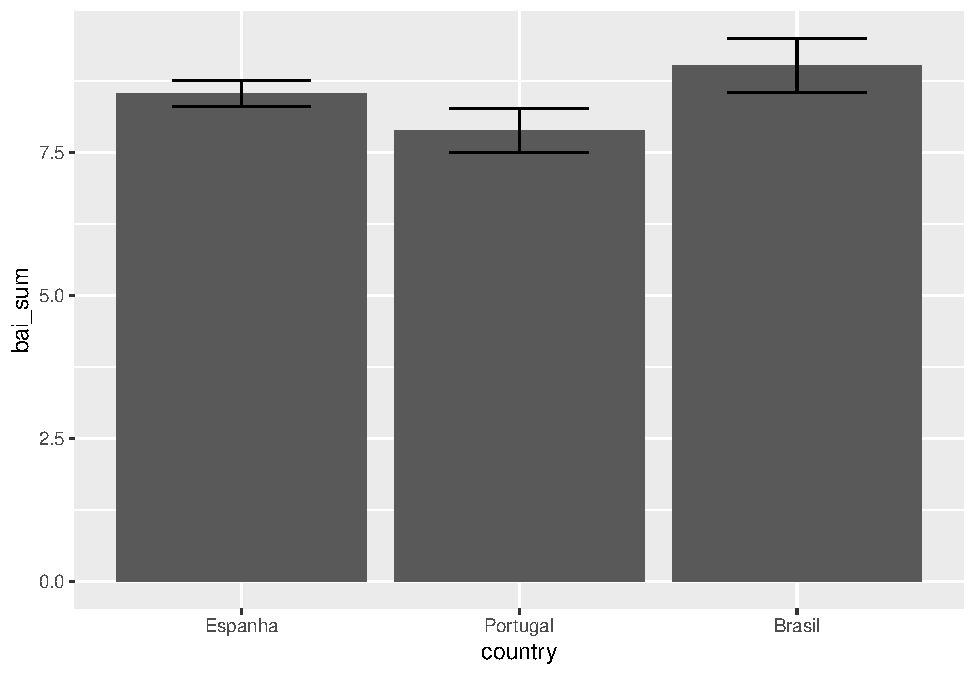
\includegraphics{gitbook-demo_files/figure-latex/unnamed-chunk-20-1} \end{center}

O boxplot a seguir também é um gráfico indicado:

\begin{Shaded}
\begin{Highlighting}[]
\KeywordTok{ggplot}\NormalTok{(Dataset, }\KeywordTok{aes}\NormalTok{(}\DataTypeTok{x =}\NormalTok{ country, }\DataTypeTok{y =}\NormalTok{ bai_sum)) }\OperatorTok{+}
\StringTok{  }\KeywordTok{geom_boxplot}\NormalTok{()}
\end{Highlighting}
\end{Shaded}

\begin{center}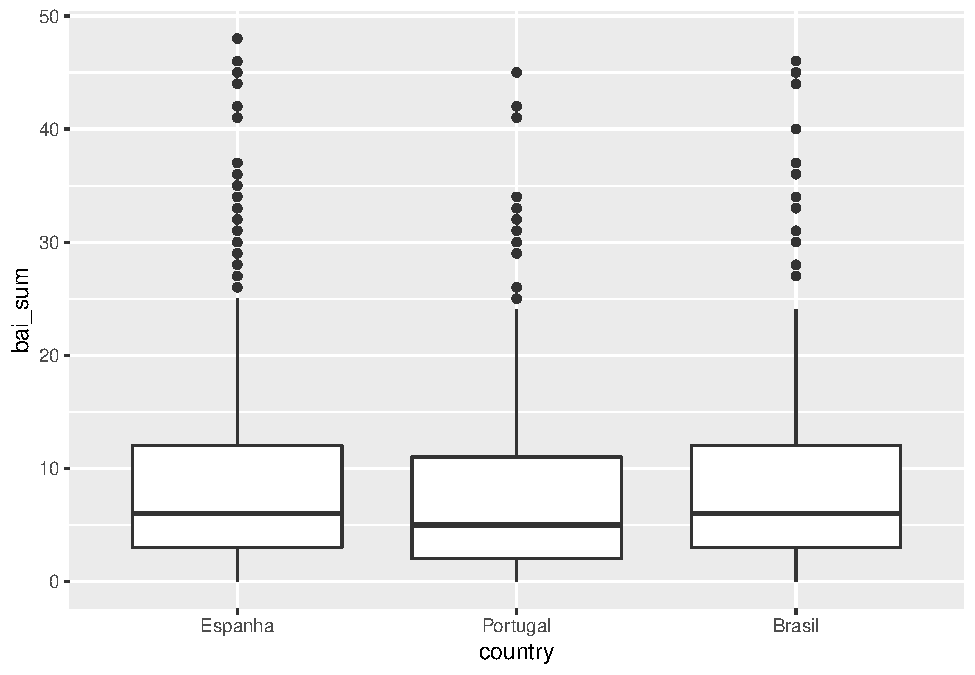
\includegraphics{gitbook-demo_files/figure-latex/unnamed-chunk-21-1} \end{center}

\hypertarget{variuxe1veis-com-vi-contuxednua-e-vd-contuxednua}{%
\section{2 variáveis com VI contínua (e VD contínua)}\label{variuxe1veis-com-vi-contuxednua-e-vd-contuxednua}}

Assumindo que a VI é contínua e a VD também, o gráfico de pontos e de dispersão são virtualmente identicos e indicados. Esses gráficos permitem verificar a \textbf{associação} entre as variáveis. No ggoplot, o argumento \texttt{geom\_point} e \texttt{geom\_jitter} são possíveis. Abaixo, utilizando os pontos.

\begin{Shaded}
\begin{Highlighting}[]
\KeywordTok{ggplot}\NormalTok{(Dataset, }\KeywordTok{aes}\NormalTok{(}\DataTypeTok{x =}\NormalTok{ age, }\DataTypeTok{y =}\NormalTok{ bai_sum)) }\OperatorTok{+}
\StringTok{  }\KeywordTok{geom_point}\NormalTok{()}
\end{Highlighting}
\end{Shaded}

\begin{verbatim}
## Warning: Removed 28 rows containing missing values (geom_point).
\end{verbatim}

\begin{center}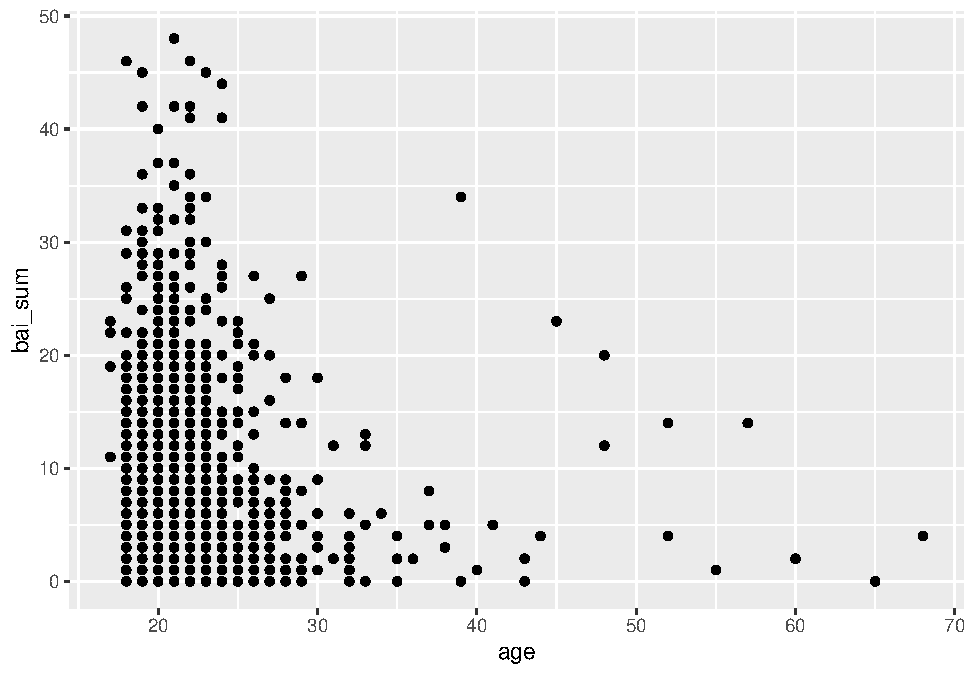
\includegraphics{gitbook-demo_files/figure-latex/unnamed-chunk-22-1} \end{center}

Abaixo, utilizando o jitter

\begin{Shaded}
\begin{Highlighting}[]
\KeywordTok{ggplot}\NormalTok{(Dataset, }\KeywordTok{aes}\NormalTok{(}\DataTypeTok{x =}\NormalTok{ age, }\DataTypeTok{y =}\NormalTok{ bai_sum)) }\OperatorTok{+}
\StringTok{  }\KeywordTok{geom_jitter}\NormalTok{()}
\end{Highlighting}
\end{Shaded}

\begin{verbatim}
## Warning: Removed 28 rows containing missing values (geom_point).
\end{verbatim}

\begin{center}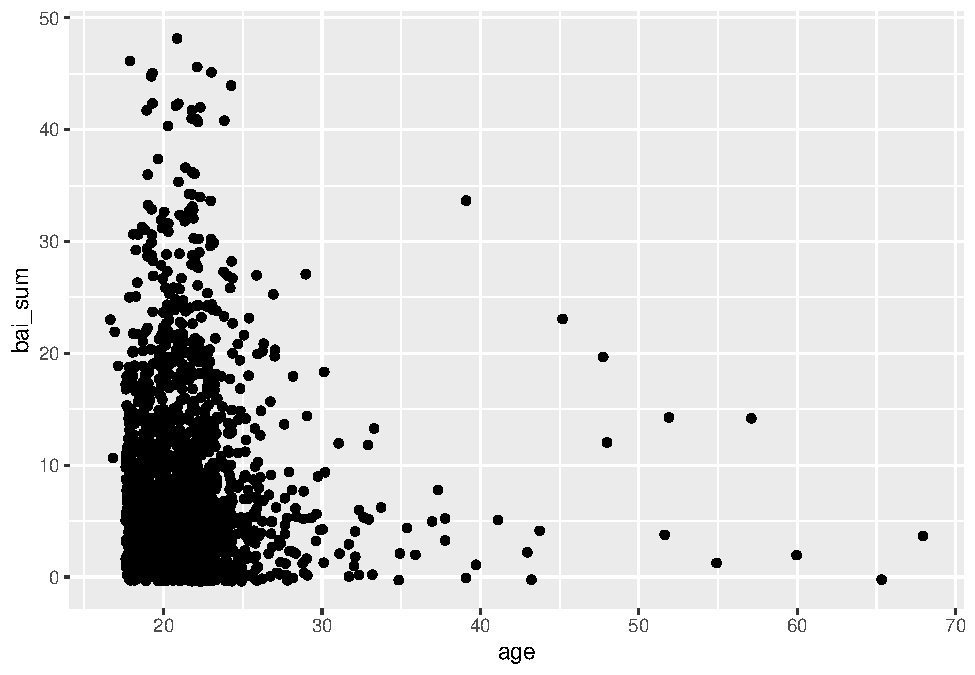
\includegraphics{gitbook-demo_files/figure-latex/unnamed-chunk-23-1} \end{center}

Tradicionalmente, de maneira análoga às barras de erros apresentadas em gráficos cujas VIs são discretas, adiciona-se uma reta de regressão amostral (fra) quando a VI é contínua, tal como apresentado a seguir.

\begin{Shaded}
\begin{Highlighting}[]
\KeywordTok{ggplot}\NormalTok{(Dataset, }\KeywordTok{aes}\NormalTok{(}\DataTypeTok{x =}\NormalTok{ age, }\DataTypeTok{y =}\NormalTok{ bai_sum)) }\OperatorTok{+}
\StringTok{  }\KeywordTok{geom_jitter}\NormalTok{() }\OperatorTok{+}
\StringTok{  }\KeywordTok{geom_smooth}\NormalTok{(}\DataTypeTok{method =} \StringTok{"lm"}\NormalTok{)}
\end{Highlighting}
\end{Shaded}

\begin{verbatim}
## `geom_smooth()` using formula 'y ~ x'
\end{verbatim}

\begin{verbatim}
## Warning: Removed 28 rows containing non-finite values (stat_smooth).
\end{verbatim}

\begin{verbatim}
## Warning: Removed 28 rows containing missing values (geom_point).
\end{verbatim}

\begin{center}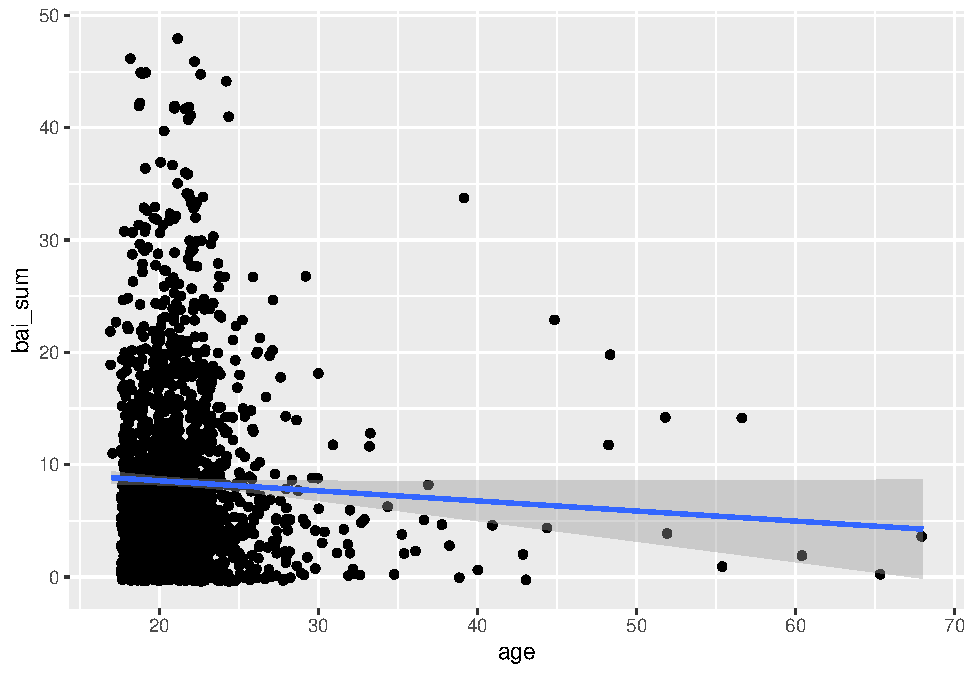
\includegraphics{gitbook-demo_files/figure-latex/unnamed-chunk-24-1} \end{center}

\hypertarget{outros-gruxe1ficos-e-configurauxe7uxf5es}{%
\section{Outros gráficos e configurações}\label{outros-gruxe1ficos-e-configurauxe7uxf5es}}

Evidentemente, é possível apresentar mais informações nos gráficos com mais de um variável apresentada, desde que elas sejam relacionadas ao problema de pesquisa estudado e não sobrecarreguem a visualização dos resultados. Frequentemente, as informações adicionais são feitas pela inclusão de \textbf{clusters} ou \textbf{agrupamentos}. Isso é tanto possível em gráficos cuja VI seja discreta quanto contínua.

No exemplo abaixo, o gráfico dos resultados do Inventário Beck de Ansiedade entre os 3 países investigados (VI discreta) agora está agrupado pelo sexo do participante.

\begin{Shaded}
\begin{Highlighting}[]
\NormalTok{Dataset }\OperatorTok\StringTok{ }
\StringTok{  }\KeywordTok{filter}\NormalTok{(}\OperatorTok{!}\KeywordTok{is.na}\NormalTok{(sex)) }\OperatorTok\StringTok{ }
\StringTok{  }\KeywordTok{ggplot}\NormalTok{(., }\KeywordTok{aes}\NormalTok{(}\DataTypeTok{x =}\NormalTok{ country, }\DataTypeTok{y =}\NormalTok{ bai_sum, }\DataTypeTok{fill =}\NormalTok{ sex)) }\OperatorTok{+}
\StringTok{  }\KeywordTok{geom_bar}\NormalTok{(}\DataTypeTok{stat =} \StringTok{"summary"}\NormalTok{, }\DataTypeTok{position =} \StringTok{"dodge"}\NormalTok{) }\OperatorTok{+}
\StringTok{  }\KeywordTok{stat_summary}\NormalTok{(}\DataTypeTok{geom=}\StringTok{"errorbar"}\NormalTok{, }\DataTypeTok{fun.data =}\NormalTok{ mean_se, }\DataTypeTok{position =} \KeywordTok{position_dodge}\NormalTok{(}\FloatTok{0.95}\NormalTok{), }\DataTypeTok{width =} \FloatTok{.5}\NormalTok{) }
\end{Highlighting}
\end{Shaded}

\begin{verbatim}
## No summary function supplied, defaulting to `mean_se()`
\end{verbatim}

\begin{center}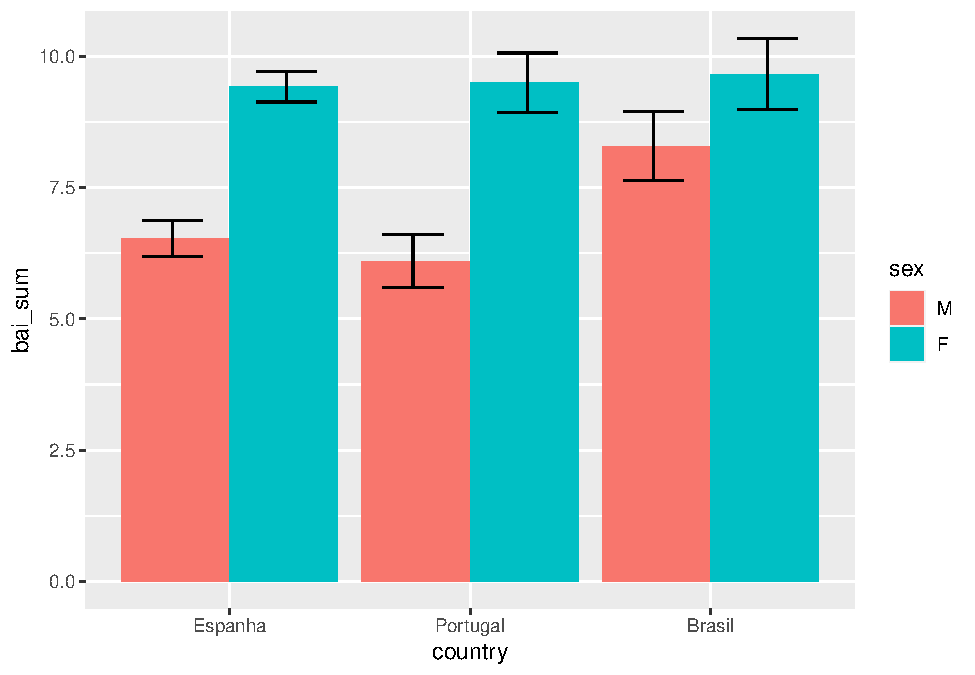
\includegraphics{gitbook-demo_files/figure-latex/unnamed-chunk-25-1} \end{center}

Já no exemplo abaixo, a relação entre idade e pontuação no Inventário Beck de Ansiedade está agora agrupada pelo sexo do participante.

\begin{Shaded}
\begin{Highlighting}[]
\NormalTok{Dataset }\OperatorTok\StringTok{ }
\StringTok{  }\KeywordTok{filter}\NormalTok{(}\OperatorTok{!}\KeywordTok{is.na}\NormalTok{(sex)) }\OperatorTok\StringTok{ }
\StringTok{  }\KeywordTok{ggplot}\NormalTok{(., }\KeywordTok{aes}\NormalTok{(}\DataTypeTok{x =}\NormalTok{ age, }\DataTypeTok{y =}\NormalTok{ bai_sum, }\DataTypeTok{color =}\NormalTok{ sex)) }\OperatorTok{+}
\StringTok{  }\KeywordTok{geom_jitter}\NormalTok{() }\OperatorTok{+}
\StringTok{  }\KeywordTok{geom_smooth}\NormalTok{(}\DataTypeTok{method =} \StringTok{"lm"}\NormalTok{) }
\end{Highlighting}
\end{Shaded}

\begin{verbatim}
## `geom_smooth()` using formula 'y ~ x'
\end{verbatim}

\begin{verbatim}
## Warning: Removed 24 rows containing non-finite values (stat_smooth).
\end{verbatim}

\begin{verbatim}
## Warning: Removed 24 rows containing missing values (geom_point).
\end{verbatim}

\begin{center}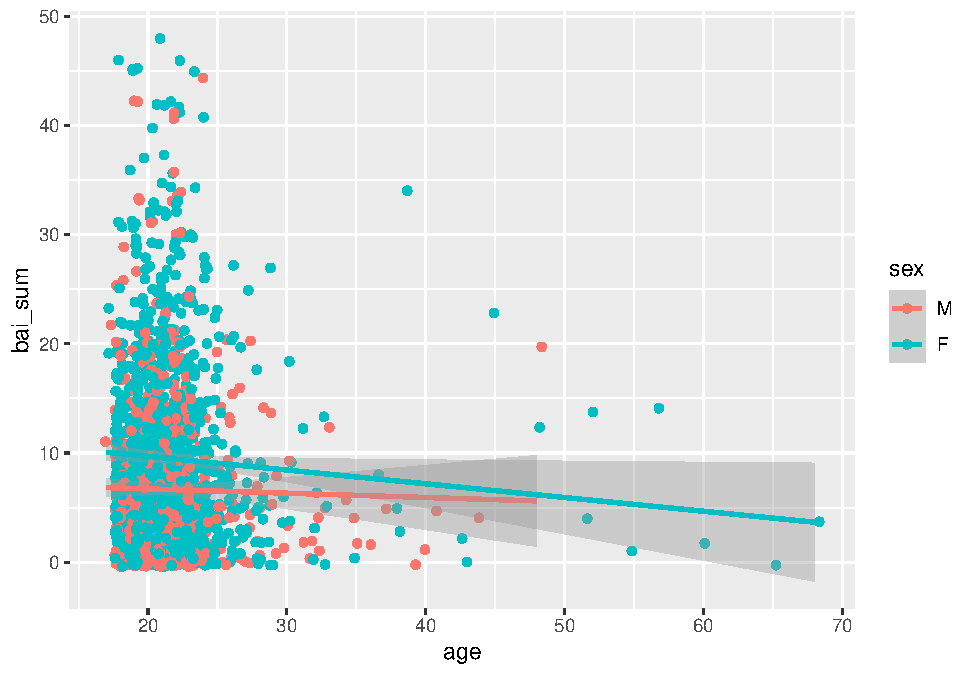
\includegraphics{gitbook-demo_files/figure-latex/unnamed-chunk-26-1} \end{center}

Em situações onde existe uma grande quantidade de informação para ser apresentada, os resultados começam a se tornar difíceis de serem entendidos. O gráfico abaixo, por exemplo, é excessivamente carregado de informação e, consequentemente, inadequado.

\begin{Shaded}
\begin{Highlighting}[]
\NormalTok{Dataset }\OperatorTok\StringTok{ }
\StringTok{  }\KeywordTok{filter}\NormalTok{(}\OperatorTok{!}\KeywordTok{is.na}\NormalTok{(sex)) }\OperatorTok\StringTok{ }
\StringTok{  }\KeywordTok{ggplot}\NormalTok{(., }\KeywordTok{aes}\NormalTok{(}\DataTypeTok{x =}\NormalTok{ age, }\DataTypeTok{y =}\NormalTok{ bai_sum, }\DataTypeTok{color =}\NormalTok{ sex, }\DataTypeTok{shape =}\NormalTok{ country)) }\OperatorTok{+}
\StringTok{  }\KeywordTok{geom_jitter}\NormalTok{() }\OperatorTok{+}
\StringTok{  }\KeywordTok{geom_smooth}\NormalTok{(}\DataTypeTok{method =} \StringTok{"lm"}\NormalTok{) }
\end{Highlighting}
\end{Shaded}

\begin{verbatim}
## `geom_smooth()` using formula 'y ~ x'
\end{verbatim}

\begin{verbatim}
## Warning: Removed 24 rows containing non-finite values (stat_smooth).
\end{verbatim}

\begin{verbatim}
## Warning: Removed 24 rows containing missing values (geom_point).
\end{verbatim}

\begin{center}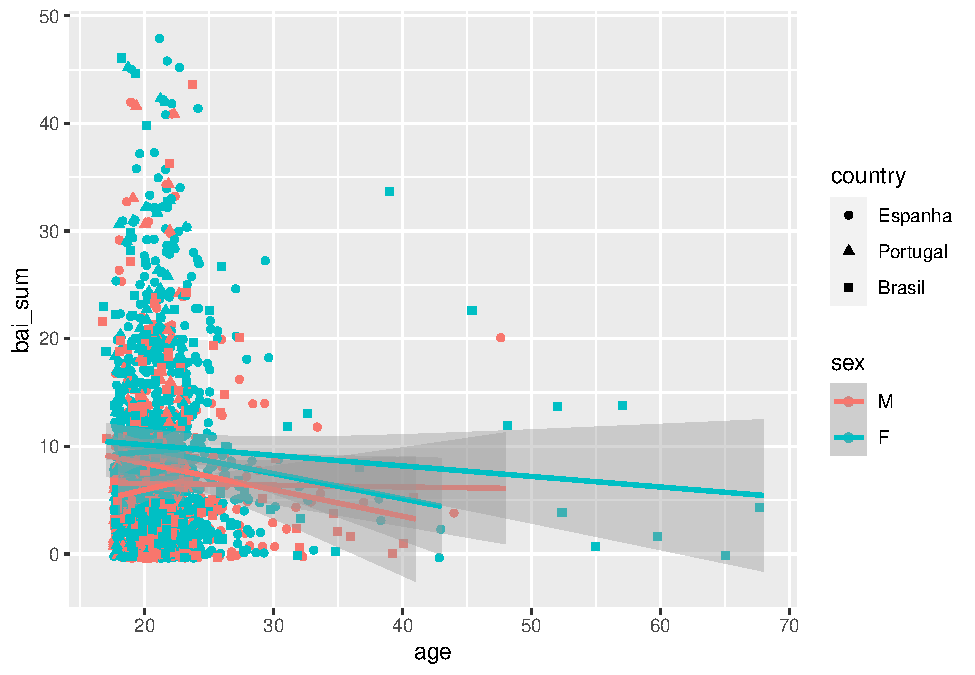
\includegraphics{gitbook-demo_files/figure-latex/unnamed-chunk-27-1} \end{center}

Em outro sentido, o gráfico a seguir quebra a apresentação dos resultados por país e, com isso, potencializa que a informação seja melhor compreendida.

\begin{Shaded}
\begin{Highlighting}[]
\NormalTok{Dataset }\OperatorTok\StringTok{ }
\StringTok{  }\KeywordTok{filter}\NormalTok{(}\OperatorTok{!}\KeywordTok{is.na}\NormalTok{(sex)) }\OperatorTok\StringTok{ }
\StringTok{  }\KeywordTok{ggplot}\NormalTok{(., }\KeywordTok{aes}\NormalTok{(}\DataTypeTok{x =}\NormalTok{ age, }\DataTypeTok{y =}\NormalTok{ bai_sum, }\DataTypeTok{color =}\NormalTok{ sex)) }\OperatorTok{+}
\StringTok{  }\KeywordTok{geom_jitter}\NormalTok{() }\OperatorTok{+}
\StringTok{  }\KeywordTok{geom_smooth}\NormalTok{(}\DataTypeTok{method =} \StringTok{"lm"}\NormalTok{) }\OperatorTok{+}
\StringTok{  }\KeywordTok{facet_wrap}\NormalTok{( }\OperatorTok{~}\StringTok{ }\NormalTok{country)}
\end{Highlighting}
\end{Shaded}

\begin{verbatim}
## `geom_smooth()` using formula 'y ~ x'
\end{verbatim}

\begin{verbatim}
## Warning: Removed 24 rows containing non-finite values (stat_smooth).
\end{verbatim}

\begin{verbatim}
## Warning: Removed 24 rows containing missing values (geom_point).
\end{verbatim}

\begin{center}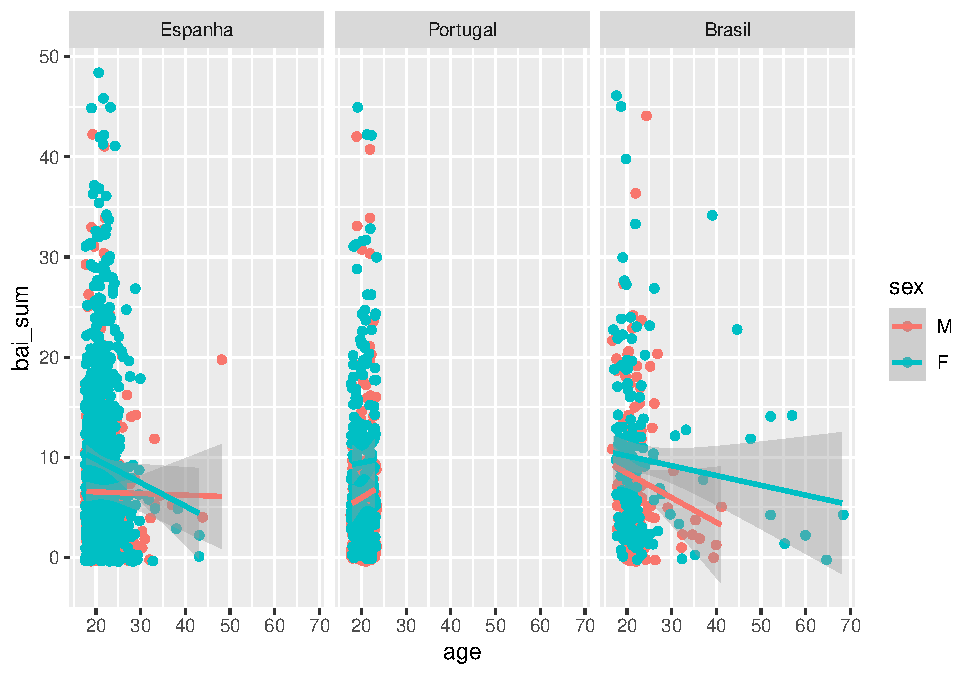
\includegraphics{gitbook-demo_files/figure-latex/unnamed-chunk-28-1} \end{center}

\hypertarget{resumo}{%
\section{Resumo}\label{resumo}}

Este capítulo apresentou os aspectos tabulares e gráficos corriqueiramente encontrados em pesquisas de Psicologia e áreas congêneres. Entre os pontos principais, a heurística típica de construção de gráficos é um conteúdo importante para ser sempre lembrado.

\hypertarget{qui-quadrado}{%
\chapter{Qui quadrado}\label{qui-quadrado}}

\begin{objectives}
\textbf{Objetivos do capítulo}\\
1. Apresentar o teste T\\
2. Discutir os pressupostos de execução do teste T\\
3. Realizar gráficos relacionados à comparação de médias\\
4. Apresentar e interpretar métricas de tamanho do efeito\\
5. Dar exemplos relacionados à escrita dos resultados 6. Apresentar
versões não paramétricas do teste T (Wilcoxon-Mann-Whitney)
\end{objectives}

\hypertarget{teste-t}{%
\chapter{Teste T}\label{teste-t}}

\begin{objectives}
\textbf{Objetivos do capítulo}\\
1. Apresentar o teste T\\
2. Discutir os pressupostos de execução do teste T\\
3. Realizar gráficos relacionados à comparação de médias\\
4. Apresentar e interpretar métricas de tamanho do efeito\\
5. Dar exemplos relacionados à escrita dos resultados 6. Apresentar
versões não paramétricas do teste T (Wilcoxon-Mann-Whitney)
\end{objectives}

O Teste T é um teste estatístico frequentemente utilizado para testar hipóteses sobre diferenças entre médias. Por utilizar dados amostrais para estimar um parâmetro (\(\mu\)), ele é um teste parâmetrico. Apenas por um preâmbulo histórico, a origem do Teste T remonta o artigo publicado em 1908 por William Gosset. Na época, em função de seu trabalho na cervejaria Guiness, ele não assinou o artigo, mas apenas usou seu pseudônimo \emph{Student}, motivo pelo qual o teste T também é chamado de Teste T de Student.

É importante notar que estudantes de Psicologia e profissionais que trabalham com avaliação psicológica costumam ser deparados com uma métrica chamada ``T score'' (Escore T, as vezes), desenvolvido em 1939 por um professor de Psicologia (William Anderson McCall). Tenha em mente que essa métrica não ter relação com os procedimentos inferenciais relacionados ao teste T a não ser uma similaridade de nome \citep{McCall1939, Krus1977}.

É possível estipular que o Teste T pode ser utilizado para comparar a média de uma amostra com a média populacional (\emph{one sample t test}), para comparar duas médias amostrais (\emph{two sample t test}), ou para comparar duas médias de uma mesma amostra que foi investigada em dois momentos do tempo (\emph{paired ou matched t test}).

Se assume os seguintes pressupostos funcionais à execução de um Teste T:

\emph{(i)} Os dados são aleatórios e representativos da população
\emph{(ii)} a variável dependente é contínua
\emph{(iii)} A distribuição dos resultados populacionais é assumida como normal

Quando há o interesse de utilizar o Teste T para comparar os resultados de dois grupos, é também necessário que:

\emph{(iv)} As variâncias dos grupos seja homogênea (princípio da homocedasticidade)
\emph{(v)} ambos os grupos sejam independentes

Quando se utiliza o Teste T pareado, se viola o princípio da independência, mas é necessário que:

\emph{(vi)} o tamanho amostral seja o mesmo

Eventualmente, quando os pressupostos são violados, versões não-paramétricas podem ser implementadas. A tabela abaixo concatena os testes estatísticos relacionados e, para fins de comparação com outros trabalhos, há autores que sugerem que se use sempre as versões não-paramétricas em resultados obtidos por processos de avaliação psicológica, arguindo que os dados têm nível de medida ``ordinal''.

\begin{longtable}[]{@{}llll@{}}
\toprule
Versão do teste & Um grupo & Dois grupos independentes & Grupos pareados\tabularnewline
\midrule
\endhead
Paramétrica & One-sample t test & Two-samples t test & Paired t test\tabularnewline
Não-paramétrica & Signed rank test & Mann-whitney & Wilcoxon\tabularnewline
\bottomrule
\end{longtable}

\hypertarget{pesquisa-1}{%
\section{Pesquisa}\label{pesquisa-1}}

\begin{alert}

Base: Livro - R - ASQ SE all age intervals

\end{alert}

Neste capítulo, vamos utilizar a pesquisa intitulada ``Confirmatory analysis and normative tables for the Brazilian Ages and Stages Questionnaires: Social--Emotional'', publicada em 2019 na Child Care Health Development. Esse trabalho teve dois objetivos. O primeiro visou confirmar a estrutura fatorial de um instrumento utilizado para avaliar competências sociais e emocionais relacionadas ao desenvolvimento infantil (ASQ:SE) e o segundo visou desenvolver tabelas normativas para comparar meninos e meninas. Essa é uma pesquisa muito importante, visto que conta com uma base de dados robusta (mais de 50 mil participantes) e costura psicometria, avaliação psicológica e políticas públicas

\hypertarget{execuuxe7uxe3o-no-r}{%
\section{Execução no R}\label{execuuxe7uxe3o-no-r}}

Como exemplo, a variável dependente do teste T tem de ser contínua. Na base de dados específica às crianças de 12 meses (\texttt{asq\_12months}), essa variável será computada pela soma de todos os itens da escala. No dplyr, isso é feito pela integração da função \texttt{mutate} com a \texttt{select}

\begin{Shaded}
\begin{Highlighting}[]
\NormalTok{asq_12months <-}\StringTok{ }\NormalTok{asq_12months }\OperatorTok\StringTok{ }
\StringTok{  }\KeywordTok{mutate}\NormalTok{(}\DataTypeTok{total_12 =} \KeywordTok{rowSums}\NormalTok{(}\KeywordTok{select}\NormalTok{(., }\KeywordTok{starts_with}\NormalTok{(}\StringTok{"q_"}\NormalTok{)), }\DataTypeTok{na.rm =} \OtherTok{TRUE}\NormalTok{))}
\end{Highlighting}
\end{Shaded}

Uma vez que o interesse é o de comparar os resultados médios obtidos por meninos e meninas aos 12 meses, é necessário a escrita adequada das hipóteses e o nível de significância adotado na análise. Dessa maneira:

\[H_0 = \mu_{meninos} - \mu_{meninas} = 0 \\ H_a = \mu_{meninos} - \mu_{meninas} \neq 0 \\ \alpha = 0.05\]

Em seguida, o processo de testagem da hipótese é feito preliminarmente de maneira gráfica e, em seguida, pela implementação do teste específico. Apesar do gráfico não ser decisivo na tomada de decisão, ele auxilia a visualilzação da distribuição da variável que temos interesse, bem como oferece já um entendimento inicial dos resultados.

Posto que a VI é discreta e a VD é continua (exposta no capítulo @ref(01-estatistica\_descritiva)) tanto o gráfico de colunas/barras como o de densidade são úteis. O gráfico de barras tem uma vantagem de ser possível adicionar barras de erros, que serão melhores descritas futuramente.

\begin{Shaded}
\begin{Highlighting}[]
\NormalTok{gridExtra}\OperatorTok{::}\KeywordTok{grid.arrange}\NormalTok{(}
  \CommentTok{#plot 1 }
  \KeywordTok{ggplot}\NormalTok{(asq_12months, }\KeywordTok{aes}\NormalTok{(}\DataTypeTok{x =}\NormalTok{ sex, }\DataTypeTok{y =}\NormalTok{ total_}\DecValTok{12}\NormalTok{, }\DataTypeTok{fill =}\NormalTok{ sex)) }\OperatorTok{+}
\StringTok{    }\KeywordTok{geom_bar}\NormalTok{(}\DataTypeTok{stat =} \StringTok{"summary"}\NormalTok{) }\OperatorTok{+}
\StringTok{    }\KeywordTok{stat_summary}\NormalTok{(}\DataTypeTok{fun.data =}\NormalTok{ mean_se, }\DataTypeTok{geom =} \StringTok{"errorbar"}\NormalTok{, }\DataTypeTok{width =} \FloatTok{.2}\NormalTok{),}
  \CommentTok{#plot 2}
    \KeywordTok{ggplot}\NormalTok{(asq_12months, }\KeywordTok{aes}\NormalTok{(}\DataTypeTok{x =}\NormalTok{ total_}\DecValTok{12}\NormalTok{, }\DataTypeTok{fill =}\NormalTok{ sex)) }\OperatorTok{+}\StringTok{ }
\StringTok{    }\KeywordTok{geom_density}\NormalTok{(}\DataTypeTok{color =} \OtherTok{NA}\NormalTok{, }\DataTypeTok{alpha=}\NormalTok{.}\DecValTok{6}\NormalTok{)}
\NormalTok{)}
\end{Highlighting}
\end{Shaded}

\begin{verbatim}
## No summary function supplied, defaulting to `mean_se()`
\end{verbatim}

\begin{center}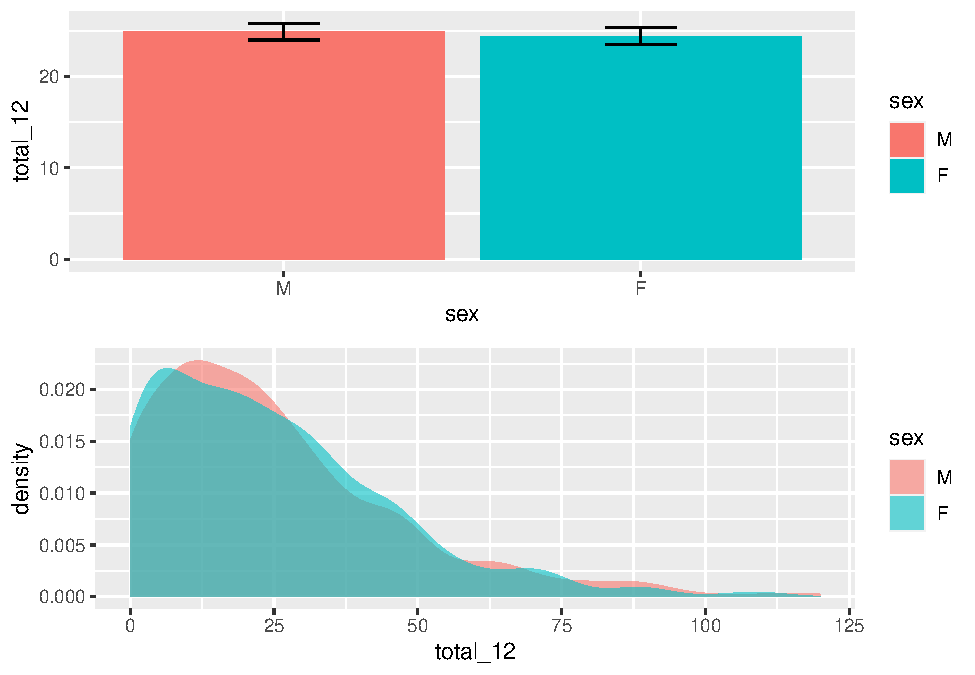
\includegraphics{gitbook-demo_files/figure-latex/unnamed-chunk-32-1} \end{center}

Feito isso, o próximo passo é a testagem formal da hipótese. Como exposto, o teste T de duas amostras independentes assume que os resultados da variável de interesse se distribua normalmente e que variância entre os grupos seja homocedástica. Tecnicamente, como o teste T é um caso especial de um modelo de regressão, a normalidade da variável de interesse se refere aos resíduos do modelo e, neste caso pode ser testada pela distribuição marginal dos resultados de ambos os grupos.

A normalidade pode ser avaliada graficamente por QQ-plots e por testes específicos, como o Shapiro-wilk, Anderson-Darling e Jarque Bera.

O QQ plot é um gráfico que reúne a distribuição empírica ordenada dos quantis conta os quantis da distribuição teórica (aqui, normal). Se os dados e a linha diagonal se soprepuserem, isso é uma evidencia de que a distribuição empírica é a mesma da distribuição teórica. Caso haja discrepância, isso aponta para desvio da normalidade.

\begin{Shaded}
\begin{Highlighting}[]
\KeywordTok{ggplot}\NormalTok{(asq_12months, }\KeywordTok{aes}\NormalTok{(}\DataTypeTok{sample =}\NormalTok{ total_}\DecValTok{12}\NormalTok{)) }\OperatorTok{+}\StringTok{ }
\StringTok{  }\KeywordTok{stat_qq}\NormalTok{()  }\OperatorTok{+}\StringTok{ }\KeywordTok{stat_qq_line}\NormalTok{() }\OperatorTok{+}
\StringTok{  }\KeywordTok{facet_wrap}\NormalTok{(}\OperatorTok{~}\NormalTok{sex)}
\end{Highlighting}
\end{Shaded}

\begin{center}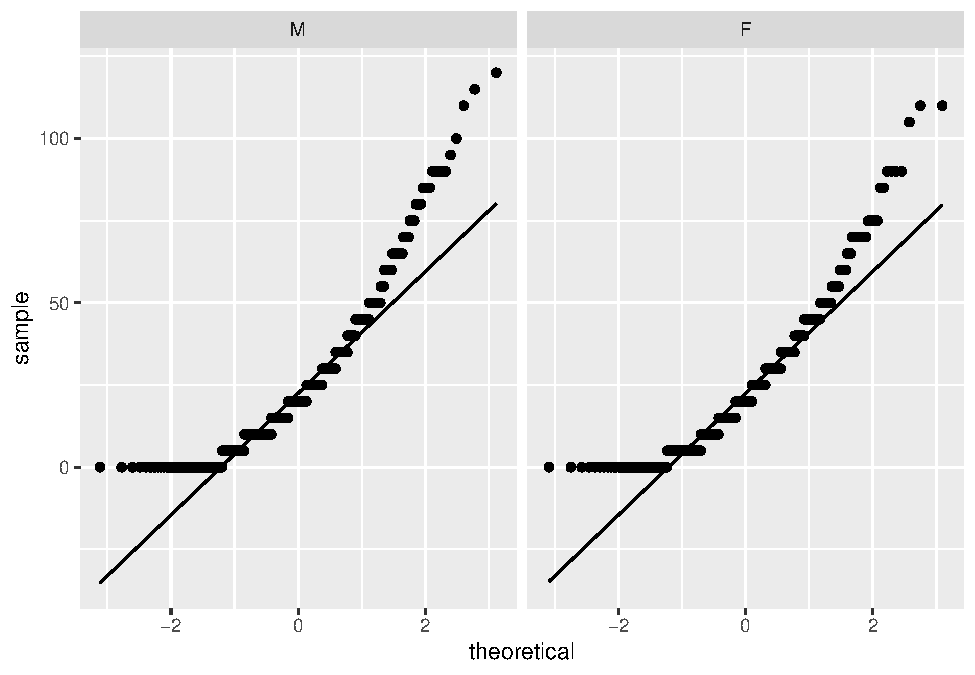
\includegraphics{gitbook-demo_files/figure-latex/unnamed-chunk-33-1} \end{center}

Apesar do gráfico já ter sido bastante claro e sugerir fortemente desvio da normalidade em ambos os grupos, o teste formal é necessário. O Shapiro-wilk costuma ser utilizado neste caso, uma vez que ele reúne diferentes características positivas no balanço entre erro do tipo 1 e 2. a Hipótese nula desse teste assume que a variável de interesse tem distribuiÇào (aproximadamente) normal. Assim, rejeitar a hipótese nula sugere que esse princípio foi violado e, com isso, o teste T pode ter resultados distorcidos.

\begin{Shaded}
\begin{Highlighting}[]
\NormalTok{asq_12months }\OperatorTok\StringTok{ }
\StringTok{  }\KeywordTok{group_by}\NormalTok{(sex) }\OperatorTok\StringTok{ }
\StringTok{  }\KeywordTok{summarise}\NormalTok{(}\DataTypeTok{shapiro =} \KeywordTok{shapiro.test}\NormalTok{(total_}\DecValTok{12}\NormalTok{)}\OperatorTok{$}\NormalTok{p.value)}
\end{Highlighting}
\end{Shaded}

\begin{verbatim}
## `summarise()` ungrouping output (override with `.groups` argument)
\end{verbatim}

\begin{verbatim}
## # A tibble: 2 x 2
##   sex    shapiro
##   <fct>    <dbl>
## 1 M     1.98e-19
## 2 F     4.80e-17
\end{verbatim}

De maneira convergente ao gráfico, o Shapiro-wilk também apontou que o princípio da normalidade foi violado. Entretanto, por finalidades didáticas, as análises continuarão.

A homogeneidade das variâncias pode ser testada visualmente e pelo teste de Bartlett ou Levene. De maneira análoga ao Shapiro-wilk, esses testes assumem como Hipótese nula a homogeneidade das variâncias. Consequemente, a rejeição desse pressuposto pode também trazer resultados distorcidos ao resultado do teste T.

\begin{Shaded}
\begin{Highlighting}[]
\KeywordTok{bartlett.test}\NormalTok{(total_}\DecValTok{12} \OperatorTok{~}\StringTok{ }\NormalTok{sex, }\DataTypeTok{data =}\NormalTok{ asq_12months)}
\end{Highlighting}
\end{Shaded}

\begin{verbatim}
## 
##  Bartlett test of homogeneity of variances
## 
## data:  total_12 by sex
## Bartlett's K-squared = 1.1357, df = 1, p-value = 0.2866
\end{verbatim}

Diferentemente do pressuposto da normalidade, o pressuposto da homocedasticidade foi preservado.\\
Agora, finalmente, o teste T.

\begin{Shaded}
\begin{Highlighting}[]
\NormalTok{(t_test_12m <-}\StringTok{ }\KeywordTok{t.test}\NormalTok{(total_}\DecValTok{12} \OperatorTok{~}\StringTok{ }\NormalTok{sex, }\DataTypeTok{var.equal =}\NormalTok{ T, }\DataTypeTok{data =}\NormalTok{ asq_12months))}
\end{Highlighting}
\end{Shaded}

\begin{verbatim}
## 
##  Two Sample t-test
## 
## data:  total_12 by sex
## t = 0.36787, df = 1039, p-value = 0.713
## alternative hypothesis: true difference in means is not equal to 0
## 95 percent confidence interval:
##  -2.077671  3.036424
## sample estimates:
## mean in group M mean in group F 
##        24.91713        24.43775
\end{verbatim}

Os resultados trazem a média de ambos os grupos (24.9171271 e 24.437751), a estatística do teste (0.3678679, as vezes chamada de T calculado), os graus de liberdade
(1039) e o valor de p 0.7130467. Repare que como o valor de p é superior ao valor estipulado do nível de significância (0.05), falha-se em rejeitar a Hipótese nula, indicando que, apesar de numericamente distintos, os resultados não são estatisticamente significativos.

\begin{writing}
\textbf{Como escrever os resultados}

Os dados foram analisados por um Teste T de amostras independentes para
investigar as diferenças médias nos resultados do desenvolvimento entre
meninos e meninas. Os resultados mostraram que os valores médios de
meninos e meninas não não são significativamente diferentes (t(1039) =
0.37, p = 0.71). Dessa maneira, as diferenças encontradas podem ser mais
bem explicadas por outras fontes de variações.
\end{writing}

Com isto concluído, é também possível verificar se existem diferenças em idades mais avançadas. A sintaxe é customizável e torna-se fácil testar a hipótese da diferença, por exemplo, aos 18 meses. Nesse sentido, o teste de hipóteses deve ser normalmente escrito:

\[H_0 = \mu_{meninos} - \mu_{meninas} = 0 \\ H_a = \mu_{meninos} - \mu_{meninas} \neq 0 \\ \alpha = 0.05\]

O gráfico novamente deve ser realizado

\begin{Shaded}
\begin{Highlighting}[]
\NormalTok{gridExtra}\OperatorTok{::}\KeywordTok{grid.arrange}\NormalTok{(}
  \KeywordTok{ggplot}\NormalTok{(asq_18months, }\KeywordTok{aes}\NormalTok{(}\DataTypeTok{x =}\NormalTok{ sex, }\DataTypeTok{y =}\NormalTok{ score, }\DataTypeTok{fill =}\NormalTok{ sex)) }\OperatorTok{+}
\StringTok{  }\KeywordTok{geom_bar}\NormalTok{(}\DataTypeTok{stat =} \StringTok{"summary"}\NormalTok{) }\OperatorTok{+}
\StringTok{  }\KeywordTok{stat_summary}\NormalTok{(}\DataTypeTok{fun.data =}\NormalTok{ mean_se, }\DataTypeTok{geom =} \StringTok{"errorbar"}\NormalTok{, }\DataTypeTok{width =} \FloatTok{.2}\NormalTok{),}

  \KeywordTok{ggplot}\NormalTok{(asq_18months, }\KeywordTok{aes}\NormalTok{(}\DataTypeTok{x =}\NormalTok{ score, }\DataTypeTok{fill =}\NormalTok{ sex)) }\OperatorTok{+}\StringTok{ }
\StringTok{  }\KeywordTok{geom_density}\NormalTok{(}\DataTypeTok{color =} \OtherTok{NA}\NormalTok{, }\DataTypeTok{alpha=}\NormalTok{.}\DecValTok{6}\NormalTok{))}
\end{Highlighting}
\end{Shaded}

\begin{verbatim}
## No summary function supplied, defaulting to `mean_se()`
\end{verbatim}

\begin{center}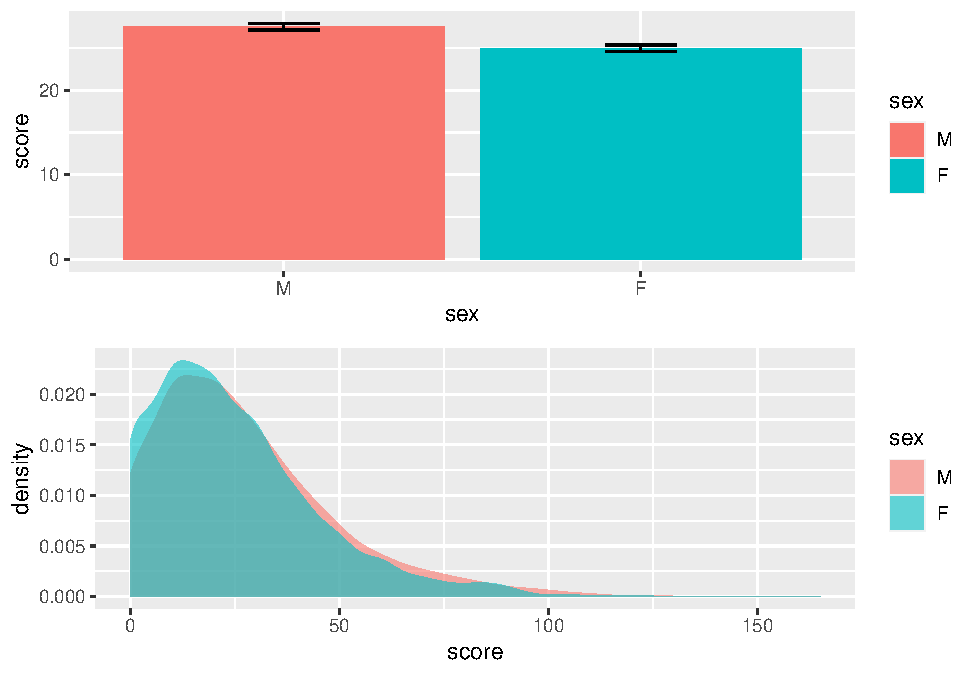
\includegraphics{gitbook-demo_files/figure-latex/unnamed-chunk-38-1} \end{center}

Bem como a verificação do pressuposto de normalidade e homocedasticidade, seguidos pelo teste formal.

\begin{Shaded}
\begin{Highlighting}[]
\NormalTok{(t_test_18m <-}\StringTok{ }\KeywordTok{t.test}\NormalTok{(score }\OperatorTok{~}\StringTok{ }\NormalTok{sex, }\DataTypeTok{var.equal =}\NormalTok{ T,}\DataTypeTok{data =}\NormalTok{ asq_18months))}
\end{Highlighting}
\end{Shaded}

\begin{verbatim}
## 
##  Two Sample t-test
## 
## data:  score by sex
## t = 4.6185, df = 5725, p-value = 3.949e-06
## alternative hypothesis: true difference in means is not equal to 0
## 95 percent confidence interval:
##  1.484680 3.674581
## sample estimates:
## mean in group M mean in group F 
##        27.52685        24.94722
\end{verbatim}

Diferentemente do anterior, agora o resultado foi significativo (p \textless{} 0.01) e deve ser reportado:

\begin{writing}
\textbf{Como escrever os resultados}

Os dados foram analisados por um Teste T de amostras independentes para
investigar as diferenças médias nos resultados do desenvolvimento entre
meninos e meninas com 18 meses idade. Os resultados mostraram que os
valores médios de meninos (M = 27.5, SD = 21.8) e meninas (M = 24.9, SD
= 20.3) são significativamente diferentes (t(5725) = 4.62, p \textless{}
0.01).
\end{writing}

É importante ter uma atenção especial à significância estatística. De forma alguma, um resultado que rejeita a hipótese nula (como o de agora) deve ser entendido como ``aceitação da hipótese alternativa'', tampouco como evidência de causalidade. É fundamental lembrar que o valor de P se refere à probabilidade de encontrar a estatística de teste calculada, ou uma ainda mais exterma, assumindo que a hipótese nula é verdadeira. Apesar de algo contra-intuitivo (e talvez desanimador), é assim que a estatística frequentista funciona.

\hypertarget{tamanho-do-efeito}{%
\section{Tamanho do efeito}\label{tamanho-do-efeito}}

Resultados significativos não são nenhum pouco informativos em relação ao tamanho do efeito. Essa métrica tem mais contato com as perguntas originalmente realizadas em uma pesquisa e é entendida como uma medida objetiva e padronizada da magnitude de um efeito observado independente da significância estatística. Assim, o tamanho do efeito pode ser considerado um indicador da relevância clínica dos grupos (em cenário biométrico, do tratamento ou condiçào).

Existem duas famílias principais no framework do tamanho do efeito, que são a família ``d'' e a família ``r''. Tecnicamente, quando comparamos médias, usamos o d de cohen para calcular a distância entre as médias das distribuições normais sobrepostas.

A interpretação é a seguinte:

\begin{longtable}[]{@{}ll@{}}
\toprule
Cohen's d & Interpretação\tabularnewline
\midrule
\endhead
d \(\geq\) 0.8 & Grande\tabularnewline
d \(\geq\) 0.5 & Moderado\tabularnewline
d \(\geq\) 0.2 & Pequeno\tabularnewline
d \textless{} 0.2 & Irrelevante\tabularnewline
\bottomrule
\end{longtable}

\begin{Shaded}
\begin{Highlighting}[]
\KeywordTok{library}\NormalTok{(effsize)}
\KeywordTok{cohen.d}\NormalTok{(score }\OperatorTok{~}\StringTok{ }\NormalTok{sex, }\DataTypeTok{data =}\NormalTok{ asq_18months)}
\end{Highlighting}
\end{Shaded}

\begin{verbatim}
## 
## Cohen's d
## 
## d estimate: 0.12216 (negligible)
## 95 percent confidence interval:
##      lower      upper 
## 0.07025972 0.17406037
\end{verbatim}

Agora é possível agregar ambos os resultados e a escrita iria por esse caminho.

\begin{writing}
\textbf{Como escrever os resultados}

Os dados foram analisados por um Teste T de amostras independentes para
investigar as diferenças médias nos resultados do desenvolvimento entre
meninos e meninas com 2 anos de idade. Os resultados mostraram que os
valores médios de meninos (M = 27.5, SD = 21.8) e meninas (M = 24.9, SD
= 20.3) são significativamente diferentes (t(5725) = 4.62, p \textless{}
0.01), apesar do tamanho do efeito ser negligenciável (d = 0.12).
\end{writing}

\hypertarget{versuxe3o-robusta-do-teste-t}{%
\section{Versão robusta do teste T}\label{versuxe3o-robusta-do-teste-t}}

Em muitas situações, os pressupostos do teste T são violados e parte da literatura argumenta que o teste T é robusto o suficiente para lidar com isso \citep{Lumley2002}, equanto outra parte sugere que é melhor optar por versões com médias aparadas ou não-paramétricas \citep{Field2017}. No entanto, o que não costuma ser discutido com tanta frequência é que a modificação do teste estatístico utilizado, necessariamente, modifica a hipótese da pesquisa. Nesse sentido, a decisão de alterar o teste estatístico deve ser feito com justificativa teórica por parte do pesquisador.

O pacote \texttt{WRS} apresenta versões robusta do Teste T. Ainda, o próprio R base oferece uma solução para condições em que a homogeneidade dos grupos não é aceita, que é o Welch-test. Esse teste é feito assumindo estipulando \texttt{var.equal\ =\ F} na sintaxe previamente exposta ou removendo este argumento por completo.

\hypertarget{mann-whitney}{%
\section{Mann-whitney}\label{mann-whitney}}

A chamada versão não paramétrica do teste T é o teste de Wilcoxon-Mann-Whitney. Quando os pressupostos do teste T são violados, o Mann-Whitney é um forte candidato para sua substituição. Se de um lado esse teste supera tais pressupostos, por outro ele responde a uma hipótese diferente daquela que o teste T trabalha. Enquanto o teste T compara médias, o Mann-whitney compara os valores ranqueados (postos). Nota-se que ele não é um teste para comparar medianas e que isso só ocorre em condições restritas.

\begin{Shaded}
\begin{Highlighting}[]
\NormalTok{(mann_whiyney_18m <-}\StringTok{ }\KeywordTok{wilcox.test}\NormalTok{(score }\OperatorTok{~}\StringTok{ }\NormalTok{sex, }\DataTypeTok{data =}\NormalTok{ asq_18months))}
\end{Highlighting}
\end{Shaded}

\begin{verbatim}
## 
##  Wilcoxon rank sum test with continuity correction
## 
## data:  score by sex
## W = 4368187, p-value = 9.902e-06
## alternative hypothesis: true location shift is not equal to 0
\end{verbatim}

Os resultados foram convergentes ao previamente encontrado e, em outras palavras, tambem apoiam a rejeição da hipótese nula. O tamanho do efeito também pode ser calculado ao implementar \(Z/\sqrt{(n)}\). O output padrão do R não oferece essa informação, mas o pacote \texttt{coin} dispõe dessa métrica.

\begin{Shaded}
\begin{Highlighting}[]
\NormalTok{coin}\OperatorTok{::}\KeywordTok{statistic}\NormalTok{(coin}\OperatorTok{::}\KeywordTok{wilcox_test}\NormalTok{(score }\OperatorTok{~}\StringTok{ }\NormalTok{sex, }\DataTypeTok{data =}\NormalTok{ asq_18months))}
\end{Highlighting}
\end{Shaded}

\begin{verbatim}
## [1] 4.41932
\end{verbatim}

Assim, implementando a fórmula, o tamanho do efeito seria aproximadamete 0.06.

\begin{writing}
\textbf{Como escrever os resultados}

Os dados foram analisados pelo teste Wilcoxon-Mann-Whitney para
investigar as diferenças nos resultados do desenvolvimento entre meninos
(Mdn = 25, IQR = 30, M = 27.53, SD = 21.61) e meninas (Mdn = 20, IQR =
25, M = 24.95, SD = 20.34) com 18 meses de idade. Os resultados
indicaram que os resultados foram significativos (W = 4368187, p
\textless{} 0.01), mas com efeito negligenciável (0.12).
\end{writing}

\hypertarget{teste-t-e-regressuxe3o}{%
\section{Teste T e regressão}\label{teste-t-e-regressuxe3o}}

Conforme alertado, o Teste T é um caso particular deum modelo de regressão que assume que a variável independente é uma dummy. Assim, \(b_0\) (intercepto) é o grupo que recebeu o valor 0 e \(b_1\) (inclinação) é o grupo que recebeu o valor 1. Caso isso não tenha sido definido inicialmente, basta estipular que a variável é um fator e o R cuidará de todo o resto.

Nesse caso, o R atribuiu os meninos como intercepto o valor médio dos meninos e a inclinação \(b_1\) é justamente a diferença entre os valores (\emph{24.95-27.53)}. Nesse caso, -2.58. A estatística F é equivalente a \(t^2\) do teste t em sua versão tradicional (assumindo variâncias iguais entre grupos, adicionando \texttt{var.equal\ =\ T} à função).

\begin{Shaded}
\begin{Highlighting}[]
\KeywordTok{lm}\NormalTok{(score }\OperatorTok{~}\StringTok{ }\NormalTok{sex, }\DataTypeTok{data =}\NormalTok{ asq_18months) }\OperatorTok\StringTok{ }
\StringTok{  }\NormalTok{stargazer}\OperatorTok{::}\KeywordTok{stargazer}\NormalTok{(., }\DataTypeTok{type =} \StringTok{"text"}\NormalTok{)}
\end{Highlighting}
\end{Shaded}

\begin{verbatim}
## 
## ===============================================
##                         Dependent variable:    
##                     ---------------------------
##                                score           
## -----------------------------------------------
## sexF                         -2.580***         
##                               (0.559)          
##                                                
## Constant                     27.527***         
##                               (0.387)          
##                                                
## -----------------------------------------------
## Observations                   5,727           
## R2                             0.004           
## Adjusted R2                    0.004           
## Residual Std. Error     21.117 (df = 5725)     
## F Statistic          21.331*** (df = 1; 5725)  
## ===============================================
## Note:               *p<0.1; **p<0.05; ***p<0.01
\end{verbatim}

\hypertarget{aspectos-matemuxe1ticos}{%
\section{Aspectos matemáticos}\label{aspectos-matemuxe1ticos}}

{[}Em desenvolvimento{]}

\hypertarget{resumo-1}{%
\section{Resumo}\label{resumo-1}}

Este capítulo introduziu a lógica por detrás do Teste T, ensinou sua execução, interpretaçào e escrita dos resultados. Frequentemente, os pressupostos que são exigidos à execução desse teste são violados e o teste de Wilcoxon-Mann-Whitney costuma ser implementado em substituição. Nesse sentido, este capítulo também apresentou os aspectos básicos deste teste. Finalmente, métricas relacionados ao tamanho do efeito foram calculadas e discutidas. É importante levar deste capítuloq que o Mann-Whitney e o teste T testam hipóteses diferentes e que significância estatística não é sinônimo de relevância clínica.

\hypertarget{anova}{%
\chapter{ANOVA}\label{anova}}

\begin{objectives}
\textbf{Objetivos do capítulo}\\
1. Apresentar a ANOVA\\
2. Discutir os pressupostos de execução da ANOVA\\
3. Realizar gráficos relacionados à comparação de médias\\
4. Apresentar e interpretar métricas de tamanho do efeito\\
5. Dar exemplos relacionados à escrita dos resultados 6. Discutir os
testes post-hoc\\
7. Apresentar versões não paramétricas da teste ANOVA (Kruskal-Wallis)
\end{objectives}

A ANOVA é um teste estatístico desenvolvimento para verificar diferença entre diversos grupos. Pragmaticamente, é possível entender ANOVA como um super teste T, onde o que está em jogo não é somente o quanto as médias amostrais estão distantes, mas o quão distantes estão relativamente à variabilidade de observações individuais.

Conceitualmente, similar ao teste T, a ANOVA e todas as suas extensões (e.g., ANCOVA e MANOVA) são casos especiais de um modelo de regressão que lidam com variáveis independente discretas/categórica.

Em Psicologia, alguns autores indicam que a ANOVA é a técnica inferencial mais utilizada \citep{Chartier2008, Howell2011}. Se por um aspecto, isso é extremamente vantajoso por estreitar a relação entre Psicologia e Estatística, por outro, isso parece ter contribuído para criação e manutenção de diferentes conceitos equivocados sobre a ANOVA.

Conceitualmente, a ANOVA é um modelo linear, tal que:

\[y_i = b_0 + b_1X{_1}_i + \epsilon_{i}\]

\(y_i\) representa a variável dependente\\
\(b_0\) é o intercepto (coeficiente linear)\\
\(b_1\) é a inclinação (coeficiente angular)\\
\(\epsilon_{i}\) é o erro/resíduo

Todos os pressupostos dos modelos linares são mantidos e o mnemônico LINE auxilia a resgatar todos eles. Assume-se que o erro é independente e identicamente distribuído (\(iid\)), distribuído normalmente com média 0 e variância constante \(\sigma^2\), ou seja: \[ \epsilon\stackrel{iid}{\sim} \mathcal{N}(\mu,\,\sigma^{2})\,\] Além de homocedástico: \[ VAR(\epsilon |x_1,x_2,...,x_k)=\sigma^2 \].\\
\texttt{iid}ainda signica erros descorrelatados \[ COV(\epsilon_1,\epsilon_j)=0 \].

É importante atentar que assumir média 0 \(E(\epsilon|x)=0\), também implica que a correlação do erro com as variáveis é nula. Operacionalmente, o erro representa todos os fatores de pesquisa e problemas de medição que afetam o resultado além das variáveis independentes consideradas na modelagem.

Da mesma forma que feito em outros capítulos, a tabela abaixo concatena os testes estatísticos relacionados quando os pressupostos são violados. Para fins de comparação com outros trabalhos, há autores que sugerem que se use sempre as versões não-paramétricas em resultados obtidos por processos de avaliação psicológica, arguindo que os dados têm nível de medida ``ordinal''.

\begin{longtable}[]{@{}lll@{}}
\toprule
Versão do teste & Um ou mais fatores & Momentos repetidos\tabularnewline
\midrule
\endhead
Paramétrica & Anova de k via(s) & Anova de medidas repetidas\tabularnewline
Não-paramétrica & Kruskal-Wallis & Teste de Friedman ou Page Test\tabularnewline
\bottomrule
\end{longtable}

A ANOVA tem diversas características de modelagem que serão descritas na seção a seguir,

\hypertarget{legenda}{%
\section{Legenda}\label{legenda}}

Diferentes termos são empregados em uma ANOVA e em modelos próximos. A legenda a seguir visa auxiliar no entendimento de cada um deles e aproximar o leitor a conceitos amplos utilizados em modelos lineares:

\begin{writing}
\textbf{Fator}: Variável independente, via, variável fonte, variável
preditora, tratamento\\
\textbf{Desfecho}: Variável dependente, variável critério\\
\textbf{Níveis}: Grupos, condições, categorias da variável
independente\\
\textbf{Efeito principal}: Efeito da variável independente, sem
considerar outras caracterísitcas do modelo\\
\textbf{Efeito de interação}: Efeito do termo de interação entre duas ou
mais variáveis independentes.Quando significativo, não se interpreta os
efeitos principais.\\
\textbf{Efeito simples}: Efeito de uma variável independente em um nível
(específico) de outra variável independente.\\
\textbf{ANCOVA}: Análise de covariância, onde se controla os resultados
por uma variável contínua \textbf{MANOVA}: Análise multivariada de
variância, onde se extende a ANOVA para incluir duas variáveis
dependentes
\end{writing}

Por heurística, se escreve os delinementos estudados por uma ANOVA com \(\eta\). Se, por exemplo, o interesse seja o de verificar o efeito do sexo (masculino ou feminino) e da escolaridade (fundamental, médio e superior), a representação será \(\eta = 2 \times 3\). Isso significa que a ANOVA tem dois fatores (sexo e escolaridade) e o primeiro fator tem dois níveis e o segundo tem 3 níveis.

\hypertarget{pesquisa-2}{%
\section{Pesquisa}\label{pesquisa-2}}

\begin{alert}

Base: Livro - R - TEG

\end{alert}

Neste capítulo, vamos utilizar a pesquisa intitulada ``A relação entre o nível de Empreendedorismo (TEG) e os aspectos sociodemográficos dos Taxistas cooperados da cidade de Santo André/São Paulo, Brasil'', publicada em 2016 na Revista Eletrônica de Gestão e Serviços, em que sou co-autor. O objetivo dessa pesquisa foi identificar o nível de empreendedorismo em 147 taxistas de Santo André/SP, bem como averiguá-lo em associação aos aspectos sociodemográficos. A base contém 14 variáveis, sendo 6 variáveis da escala utilizada para avaliação do empreendedorismo e 8 variáveis gerais, incluindo aqui os aspectos sociodemográficos, como sexo e escolaridade. Essa base será utilizada para realizar uma ANOVA de 1 via, 2 vias e uma ANOVA fatorial.

\hypertarget{anova-de-1-via}{%
\section{ANOVA de 1 via}\label{anova-de-1-via}}

A pergunta que temos agora é sobre o possível efeito da \texttt{escolaridade} na Tendência Empreendedora Geral (\texttt{teg}). Trata-se de uma ANOVA de 1 via, dado que existe apenas uma VI, com mais de 2 níveis.

\hypertarget{execuuxe7uxe3o-no-r-1}{%
\subsection{Execução no R}\label{execuuxe7uxe3o-no-r-1}}

Ao trabalhar no R, é fundamental se certificar que os tipos das variáveis estão corretamente definidos em função da escala de medida utilizada. Erros nessa etapa podem gerar resultados absolutamente incorretos. A escolaridade é uma variável categórica (ordinal, tratada como discreta) e é necessário definir claramente isso ao R antes da análise propriamente dita.

Isso pode ser feito pela função \texttt{case\_when} e \texttt{levels}. O \texttt{case\_when} irá substituir os valores originalmente presentes nessa variável e o \texttt{levels} deixará claro a ordem de cada categoria, o que é útil para que os gráficos sejam feitos corretamente.

\begin{Shaded}
\begin{Highlighting}[]
\NormalTok{dados_teg <-}\StringTok{ }\NormalTok{dados_teg }\OperatorTok\StringTok{ }
\StringTok{  }\KeywordTok{mutate_at}\NormalTok{(}\KeywordTok{vars}\NormalTok{(escolaridade), }
    \OperatorTok{~}\KeywordTok{factor}\NormalTok{(}\KeywordTok{case_when}\NormalTok{(}
\NormalTok{      . }\OperatorTok{==}\StringTok{ }\DecValTok{1} \OperatorTok{~}\StringTok{ "Primário"}\NormalTok{,}
\NormalTok{      . }\OperatorTok{==}\StringTok{ }\DecValTok{2} \OperatorTok{~}\StringTok{ "Ginásio"}\NormalTok{,}
\NormalTok{      . }\OperatorTok{==}\StringTok{ }\DecValTok{3} \OperatorTok{~}\StringTok{ "Colegial"}\NormalTok{,}
\NormalTok{      . }\OperatorTok{==}\StringTok{ }\DecValTok{4} \OperatorTok{~}\StringTok{ "Superior"}\NormalTok{), }
      \DataTypeTok{levels=}\KeywordTok{c}\NormalTok{(}\StringTok{"Primário"}\NormalTok{,}\StringTok{"Ginásio"}\NormalTok{,}\StringTok{"Colegial"}\NormalTok{,}\StringTok{"Superior"}\NormalTok{)))}
\end{Highlighting}
\end{Shaded}

Uma vez que os itens de um instrumento sociodemográfico devem levar em consideração o contexto das pessoas avaliadas e, as categorias de escolaridade foram definidas como as apresentadas. Primário significa escolaridade até o 5º ano, ginásio significa escolaridade até o 9º ano e colegial é equivalente ao ensino médio.

As hipóteses precisam ser descritas:

\[H_0 = \mu_{escolaridade_i} - \mu_{escolaridae_j} = 0 \\ H_a = c.c \\ \alpha = 0.05\]
Aqui, o subscrito \(i\) e \(j\) foi utilizado de maneira liberal para apresentar a diferença entre todas as combinações lineares possíveis.

Em seguida, a apresentação tabular das médias e desvios-padrão pode ser realizada.

\begin{Shaded}
\begin{Highlighting}[]
\NormalTok{dados_teg }\OperatorTok\StringTok{ }
\StringTok{  }\KeywordTok{group_by}\NormalTok{(escolaridade) }\OperatorTok\StringTok{ }
\StringTok{  }\KeywordTok{summarise_at}\NormalTok{(}\KeywordTok{vars}\NormalTok{(teg), }\KeywordTok{lst}\NormalTok{(}\DataTypeTok{n=}\OperatorTok{~}\KeywordTok{n}\NormalTok{(),mean,sd)) }\OperatorTok\StringTok{ }
\StringTok{  }\KeywordTok{kable}\NormalTok{(}\DataTypeTok{digits =} \DecValTok{2}\NormalTok{) }\OperatorTok\StringTok{ }\KeywordTok{kable_styling}\NormalTok{(}\DataTypeTok{bootstrap_options =} \KeywordTok{c}\NormalTok{(}\StringTok{"striped"}\NormalTok{, }\StringTok{"hover"}\NormalTok{, }\StringTok{"condensed"}\NormalTok{))}
\end{Highlighting}
\end{Shaded}

escolaridade

n

mean

sd

Primário

6

24.67

4.63

Ginásio

33

26.76

3.86

Colegial

85

28.87

4.11

Superior

23

31.83

5.23

Tal como ilustrado no decorrer dos outros capítulos, gráficos são fundamentais para entendimento do relacionamento entre as variáveis. Uma vez que a escolaridade (VI) é tratada como discreta e a TEG (VD) é contínua, um gráfico de barras é adequado. A inclusão das barras de erro permite uma compreensão inferencial inicial.

\begin{Shaded}
\begin{Highlighting}[]
\KeywordTok{ggplot}\NormalTok{(dados_teg, }\KeywordTok{aes}\NormalTok{(}\DataTypeTok{x=}\NormalTok{escolaridade, }\DataTypeTok{y =}\NormalTok{ teg, }\DataTypeTok{fill =}\NormalTok{ escolaridade)) }\OperatorTok{+}
\StringTok{  }\KeywordTok{geom_bar}\NormalTok{(}\DataTypeTok{stat =} \StringTok{"summary"}\NormalTok{) }\OperatorTok{+}
\StringTok{  }\KeywordTok{stat_summary}\NormalTok{(}\DataTypeTok{fun.data =}\NormalTok{ mean_se, }\DataTypeTok{geom =} \StringTok{"errorbar"}\NormalTok{) }\OperatorTok{+}
\StringTok{  }\KeywordTok{theme}\NormalTok{(}\DataTypeTok{legend.position =} \StringTok{"none"}\NormalTok{)}
\end{Highlighting}
\end{Shaded}

\begin{center}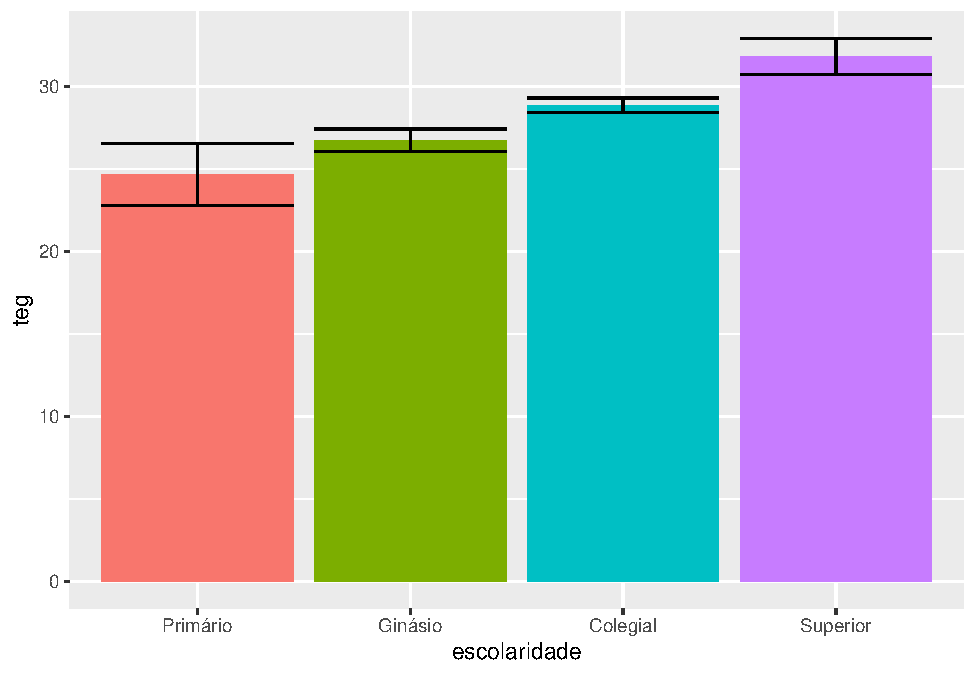
\includegraphics{gitbook-demo_files/figure-latex/unnamed-chunk-52-1} \end{center}

A visualização dos resultados já permite identificar algumas caracteríticas gerais. Primeiro, quão maior a escolaridade, maior o o valor obtido na escala. Segundo, algumas barras de erros estão superpostas e outras não, o que nos leva à conclusão preliminar de que resultados significativos estarão presentes na próxima etapa, que é a modelagem formal dessa hipótese.

A modelagem formal irá contemplar n-1 níveis dos preditores e estipulará no intercepto o nível de referência. Dessa maneira:

\[y_{i} = b_{0} + b_1Esc_{ginasio_i} + b_2Esc_{colegial_i} + b_1Esc_{superior_i} + \epsilon_{i}\]

\(b_0\) representa o intercepto, que aqui é o valor médio da Escolaridade primária\\
\(b_i\) representa os outros preditores\\
\(\epsilon_{it}\) representa o erro

A função \texttt{lm} será utilizada e o objeto \texttt{mod\_escolaridade} será armazenado. É também possível utilizar a função \texttt{aov} e a escolha da \texttt{lm} foi apenas por conveniência.

\begin{Shaded}
\begin{Highlighting}[]
\NormalTok{mod_escolaridade <-}\StringTok{ }\KeywordTok{lm}\NormalTok{(teg }\OperatorTok{~}\StringTok{ }\NormalTok{escolaridade, dados_teg)}
\end{Highlighting}
\end{Shaded}

Antes de checar os resultados, é necessário verificar se os pressupostos da ANOVA foram atendidos. Esses pedem que os resíduos sejam normalmente distribuídos e homocedásticos. Tal como previamente exposto no teste T, a investigação dessas condições é tanto feita por gráficos e testes formais e ambos são muito úteis. A análise da normalidade dos resíduos será inicialmente feita.

O gráfico abaixo apresenta a distribuição dos resíduos:

\begin{Shaded}
\begin{Highlighting}[]
\KeywordTok{ggplot}\NormalTok{(}\KeywordTok{fortify}\NormalTok{(mod_escolaridade), }\KeywordTok{aes}\NormalTok{(.resid)) }\OperatorTok{+}
\StringTok{      }\KeywordTok{geom_histogram}\NormalTok{(}\DataTypeTok{colour=}\StringTok{"black"}\NormalTok{, }\DataTypeTok{fill=}\StringTok{"grey"}\NormalTok{) }\OperatorTok{+}
\StringTok{      }\KeywordTok{geom_density}\NormalTok{(}\KeywordTok{aes}\NormalTok{(}\DataTypeTok{y=}\NormalTok{ ..count..))}
\end{Highlighting}
\end{Shaded}

\begin{center}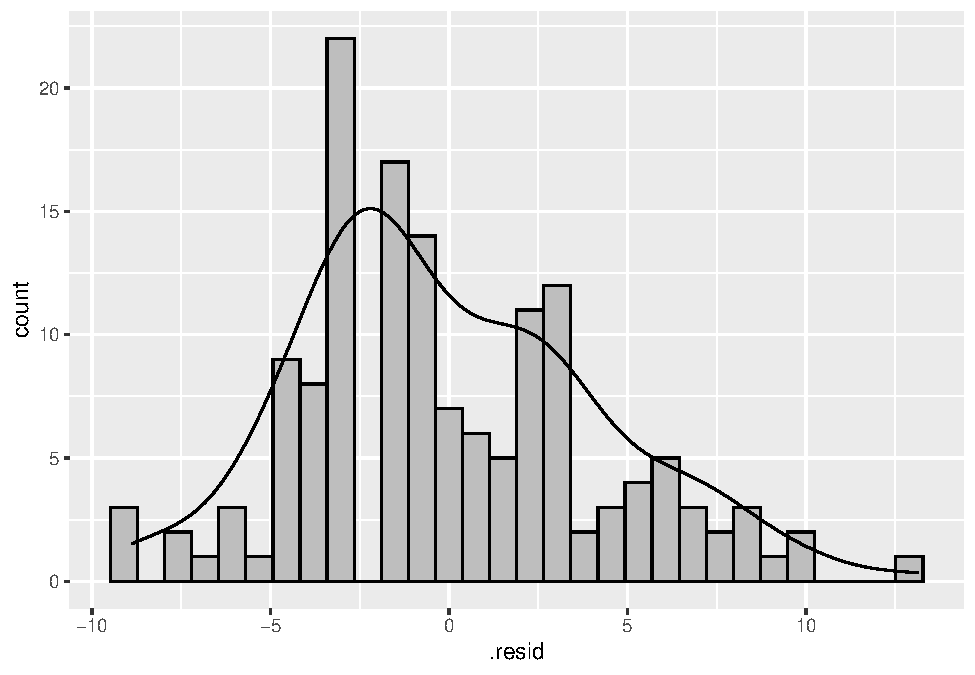
\includegraphics{gitbook-demo_files/figure-latex/unnamed-chunk-54-1} \end{center}

O teste formal pode ser feito via shapiro-wilk. Tal como no teste T, a \(H_0\) desse teste assume normalidade e, idealmente, não deve ser rejeitada.

\begin{Shaded}
\begin{Highlighting}[]
\KeywordTok{shapiro.test}\NormalTok{(}\KeywordTok{residuals}\NormalTok{(mod_escolaridade))}
\end{Highlighting}
\end{Shaded}

\begin{verbatim}
## 
##  Shapiro-Wilk normality test
## 
## data:  residuals(mod_escolaridade)
## W = 0.97502, p-value = 0.008721
\end{verbatim}

Uma vez que o valor foi menor do que o previamente estipulado ao \(\alpha\), é possível concluir que o pressuposto da normalidade foi violado. situações como essa são muito frequentes. Na literatura, são presentes recomendações de ajuste dos dados por alguma função \texttt{g(.)} ou tornar mais severo o valor de p na interpretação dos resultados. Por exemplo, em vez de 0.05, usar 0.01.

A homocedasticidade pode ser verificada por um gráfico dos resíduos contra os valores previstos. O ideal é não encontrar padrões no gráfico.

\begin{Shaded}
\begin{Highlighting}[]
\KeywordTok{ggplot}\NormalTok{(}\KeywordTok{fortify}\NormalTok{(mod_escolaridade), }\KeywordTok{aes}\NormalTok{(}\DataTypeTok{x=}\NormalTok{.fitted, }\DataTypeTok{y=}\NormalTok{.resid)) }\OperatorTok{+}\StringTok{ }
\StringTok{  }\KeywordTok{geom_point}\NormalTok{() }\OperatorTok{+}
\StringTok{  }\KeywordTok{geom_hline}\NormalTok{(}\DataTypeTok{yintercept =} \DecValTok{0}\NormalTok{)}
\end{Highlighting}
\end{Shaded}

\begin{center}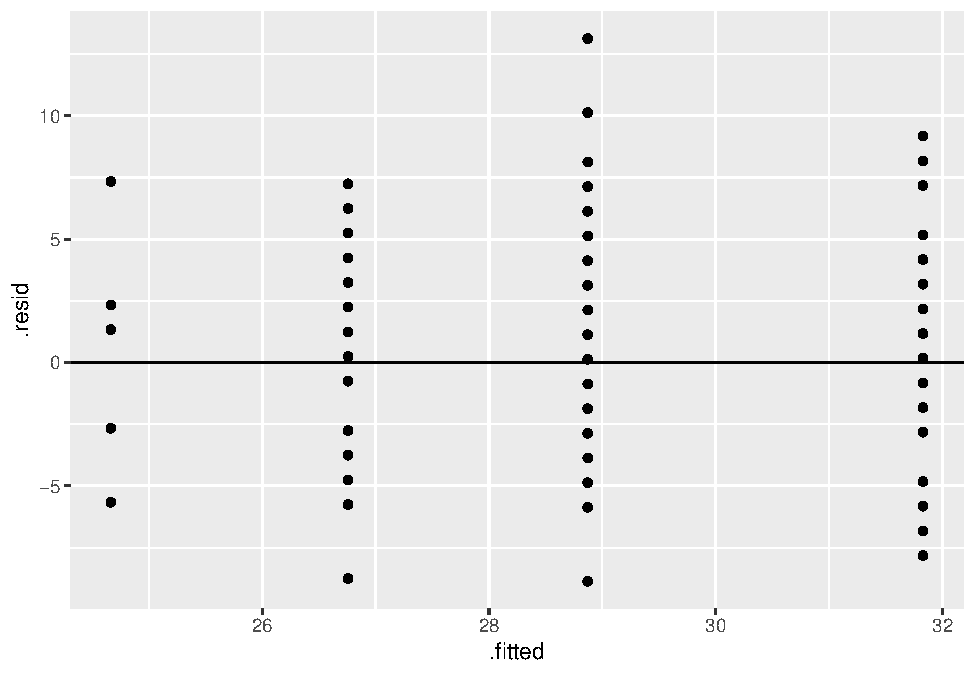
\includegraphics{gitbook-demo_files/figure-latex/unnamed-chunk-56-1} \end{center}

Além do teste de Bartlett ou Levene, em que estipulam \(H_0\) como homocedasticidade e, idealmente, não deve ser rejeitada.

\begin{Shaded}
\begin{Highlighting}[]
\NormalTok{car}\OperatorTok{::}\KeywordTok{leveneTest}\NormalTok{(mod_escolaridade)}
\end{Highlighting}
\end{Shaded}

\begin{verbatim}
## Levene's Test for Homogeneity of Variance (center = median)
##        Df F value Pr(>F)
## group   3  1.1372 0.3362
##       143
\end{verbatim}

A homocedasticidade foi assumida. Dessa maneira, mesmo com a violação da normalidade, o modelo será utilizado e seu sumário geral será apresentado pela função apa.aov do pacote \texttt{apaTables}. Isso é importante para garantir resultados programas tipicamente utilizados, como o SPSS e o STATA. Essa tabela é padronizada e muito similar na maioria dos programas estatísticos. Ela traz as seguintes informações principais:

\begin{longtable}[]{@{}lllll@{}}
\toprule
Preditor & Soma dos Quadrados & Graus de liberdade & Quadrado médio & Estat. F\tabularnewline
\midrule
\endhead
Fator & Entre (SSB) & K-1 & MSB = SSB/ k-1 & F = MSB/MSW\tabularnewline
Resíduo & Dentro (SSW) & N-k & MSW = SSW/ N-K &\tabularnewline
Total & Total (SQT) & N-1 & &\tabularnewline
\bottomrule
\end{longtable}

Aqui, K significa quantidade de categorias dentro de um fator e N significa a quantidade de observações consideradas. As siglas em inglês são comumeiramente utilizadas falar falar da ``Soma dos quadrados entre os grupos'' (SSB), ``Soma dos quadrados dentro dos grupos'' (SSW), ``Quadrado médio entre grupos'' (MSB) e ``Quadrado médio dentro dos grupos'' (MSW). Repare também que,a este momento, os aspectos são apenas apresentados conceitualmente e não matematicamente. Em outro momento, aspectos da decomposição da variância serão também descritos.

\begin{Shaded}
\begin{Highlighting}[]
\NormalTok{apaTables}\OperatorTok{::}\KeywordTok{apa.aov.table}\NormalTok{(mod_escolaridade)}
\end{Highlighting}
\end{Shaded}

\begin{verbatim}
## 
## 
## ANOVA results using teg as the dependent variable
##  
## 
##     Predictor      SS  df      MS      F    p partial_eta2 CI_90_partial_eta2
##   (Intercept) 3650.67   1 3650.67 200.61 .000                                
##  escolaridade  449.33   3  149.78   8.23 .000          .15         [.06, .22]
##         Error 2602.27 143   18.20                                            
## 
## Note: Values in square brackets indicate the bounds of the 90% confidence interval for partial eta-squared
\end{verbatim}

A leitura desse resultado é similar a de um modelo de regressão e a de outros modelos lineares e, em linhas gerais, em relatório ou publicações quase sempre apenas se diz que o modelo foi significativo, indicando as principais estatísticas obtidas da seguinte maneira: F(3,143) = 8.231, p \textless{} 0.01, ηp2 = 0.15, 90\% CI {[}.06, .22{]}.

No entanto, o que essa constatação está realmente dizendo é que houve uma comparação entre dois modelos, um que usou os resultados da variável ``escolaridade'' para prever os resultados obtidos pelo TEG (chamado de Modelo aumentado) e outro que usou apenas a média que o TEG (chamado de modelo compacto ou nulo neste caso). O resultado significativo indica que a inclusão da ``escolaridade'' no modelo testado foi significativamente capaz de reduzir o erro de previsão que o modelo nulo obteve (em ingles Proportional Reduction in Error ou PRE). Ainda nesse caso, o ηp2 (eta parcial quadrado) indica a proporção da variabilidade dos resultados do TEG que pode ser atribuídos à escolaridade e é uma métrica de tamanho do efeito, cuja interpretação se recomenda da seguinte maneira:

ηp2 \textbar{} Interpretação \textbar{} :----- :----- \textbar{} ηp2 \(\geq\) 0.14 \textbar{} Grande \textbar{} ηp2 \(\geq\) 0.06 \textbar{} Moderado \textbar{} ηp2 \(\geq\) 0.01 \textbar{} Pequeno \textbar{} ηp2 \textless{} 0.01 \textbar{} Irrelevante

De fato, quando isso ocorre, a busca por possíveis diferenças entre todas as comparações possíveis costuma ser feita por testes post hocs.

Entretanto, é importante mencionar que que se uma ANOVA é significativa, isso não significa necessariamente que haverá alguma diferença entre as médias dos grupos. Tecnicamente, a diferença pode ocorrer em qualquer comparação possível, como grupo 1 contra grupos 2 + grupo 3 ou grupo 2 contra grupo 1+3. Dessa forma, o resultado geral da ANOVA e testes post hoc respondem questões diferentes e é possível realizar qualquer comparação múltipla sem sequer realizar a ANOVA, desde que os resultados sejam devidamente corrigidos caso se assuma alguns pressupostos sobre os constrastes.

Uma vez que realizar uma ANOVA não é tecnicamente necessário para realização de comparações pareadas, é possível que alguém se pergunte qual é, então, a necessidade da realização deste primeiro teste. De fato, hoje em dia, a realização da ANOVA ocorre mais para que o pesquisador (i) consiga realizar computacionalmente todas as comparações pareadas entre as categorias da variável e, em seguida, (ii) corrigir adequadamente o valor de P obtido em cada computação.

Isso dito, uma vez que a escolaridade foi significativa, as principais comparações serão testadas dois a dois.Sempre que múltiplas que comparações são realizadas, é esperado que haja uma inflação do erro do tipo 1 e, por isso, é necessário ajustar o valor de P. Repare que a quantidade de comparações pode ser calculada da seguinte forma:

\[ J*(\frac{J-1}2) \] , onde
\(J\) é a quantidade de níveis da variável

Nesse caso:

\[ 4*(\frac{3}2) = 6 \].

Para a comparação pareada, o pacote \texttt{emmeans} será utilizado.

\hypertarget{post-hoc}{%
\subsection{Post hoc}\label{post-hoc}}

A mecanica do por detrás do post hoc é a comparação pareada de todos os níveis presentes no fator, seguido pelo ajuste do valor de P. Existem muitas técnicas para tal ajuste e elas costumam ser agrupadas em função da sua robustez à violação da homocedasticidade. Para fins práticos, vamos utilizar uma técnica considerada bastante conservadora, chamada de Bonferroni, que multiplica o valor bruto encontrado pela quantidade de comparações.

O resultado das comparações dois a dois será armazenado em um objeto específico, nomeado como \texttt{post\_hoc\_escolaridade}. Isso será útil para apresentar sumários e gráficos.

\begin{Shaded}
\begin{Highlighting}[]
\KeywordTok{library}\NormalTok{(emmeans)}
\end{Highlighting}
\end{Shaded}

\begin{Shaded}
\begin{Highlighting}[]
\NormalTok{post_hoc_escolaridade <-}\StringTok{ }\KeywordTok{emmeans}\NormalTok{(mod_escolaridade, }\StringTok{"escolaridade"}\NormalTok{) }\OperatorTok\StringTok{ }\KeywordTok{pairs}\NormalTok{(., }\DataTypeTok{reverse =} \OtherTok{TRUE}\NormalTok{, }\DataTypeTok{adjust =} \StringTok{"bonferroni"}\NormalTok{)}
\end{Highlighting}
\end{Shaded}

Tal como feito até agora, o gráfico inicial das comparações será realizado. A adição das barras de erro gera interpretação mais rápida e simples para todas as comparações.

\begin{Shaded}
\begin{Highlighting}[]
\NormalTok{CI <-}\StringTok{ }\KeywordTok{confint}\NormalTok{(post_hoc_escolaridade)}
\KeywordTok{ggplot}\NormalTok{(}\DataTypeTok{mapping =} \KeywordTok{aes}\NormalTok{(contrast, estimate)) }\OperatorTok{+}
\StringTok{  }\KeywordTok{geom_errorbar}\NormalTok{(}\KeywordTok{aes}\NormalTok{(}\DataTypeTok{ymin =}\NormalTok{ lower.CL, }\DataTypeTok{ymax =}\NormalTok{ upper.CL), }\DataTypeTok{data =}\NormalTok{ CI) }\OperatorTok{+}
\StringTok{  }\KeywordTok{geom_point}\NormalTok{(}\DataTypeTok{data =} \KeywordTok{summary}\NormalTok{(post_hoc_escolaridade)) }\OperatorTok{+}
\StringTok{  }\KeywordTok{geom_hline}\NormalTok{(}\DataTypeTok{yintercept =} \DecValTok{0}\NormalTok{, }\DataTypeTok{linetype =} \StringTok{"dashed"}\NormalTok{) }\OperatorTok{+}\StringTok{ }
\StringTok{  }\KeywordTok{scale_size}\NormalTok{(}\DataTypeTok{trans =} \StringTok{"reverse"}\NormalTok{) }\OperatorTok{+}\StringTok{ }
\StringTok{  }\KeywordTok{coord_flip}\NormalTok{()}
\end{Highlighting}
\end{Shaded}

\begin{center}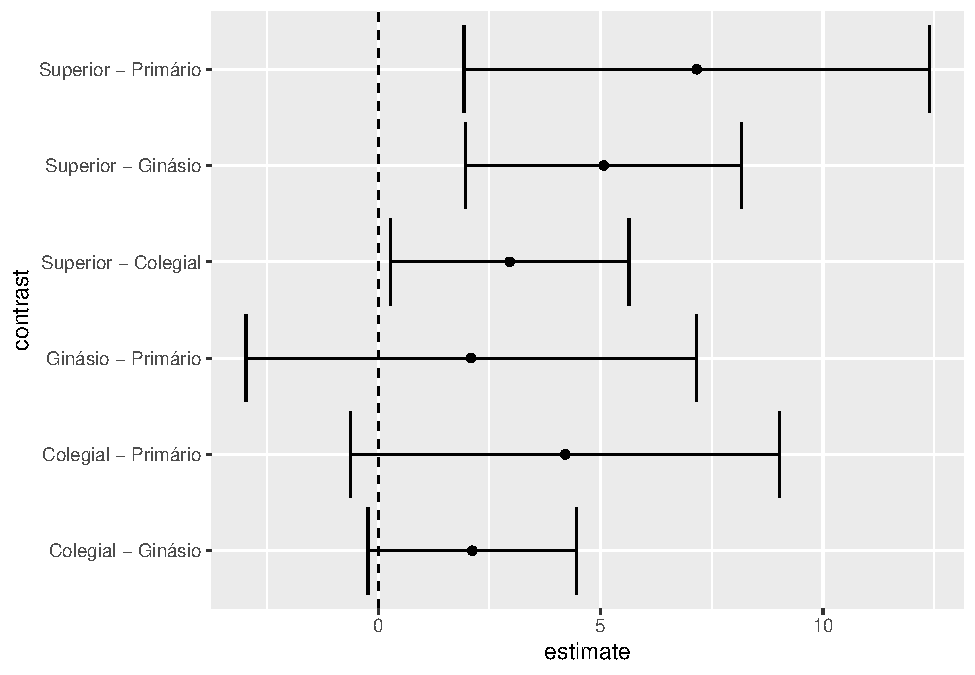
\includegraphics{gitbook-demo_files/figure-latex/unnamed-chunk-61-1} \end{center}

A apresentação tabular é fundamental e apresenta as estatísticas inferenciais de interesse:

\begin{Shaded}
\begin{Highlighting}[]
\NormalTok{post_hoc_escolaridade }\OperatorTok\StringTok{ }
\StringTok{  }\KeywordTok{kable}\NormalTok{(}\DataTypeTok{digits =} \DecValTok{2}\NormalTok{) }\OperatorTok\StringTok{ }\KeywordTok{kable_styling}\NormalTok{(}\DataTypeTok{bootstrap_options =} \KeywordTok{c}\NormalTok{(}\StringTok{"striped"}\NormalTok{, }\StringTok{"hover"}\NormalTok{, }\StringTok{"condensed"}\NormalTok{))}
\end{Highlighting}
\end{Shaded}

contrast

estimate

SE

df

t.ratio

p.value

Ginásio - Primário

2.09

1.89

143

1.10

1.00

Colegial - Primário

4.20

1.80

143

2.33

0.13

Colegial - Ginásio

2.11

0.87

143

2.42

0.10

Superior - Primário

7.16

1.96

143

3.66

0.00

Superior - Ginásio

5.07

1.16

143

4.37

0.00

Superior - Colegial

2.96

1.00

143

2.95

0.02

Os resultados são significativos na comparação \texttt{Superior\ -\ Primário}, \texttt{Superior\ -\ Ginásio} e \texttt{Superior\ -\ Colegial}. Em todos, os resultados do TEG foi mais elevado naqueles participantes que haviam concluído o ensino superior.

A esse momento, a escrita é fundamental:

\begin{writing}
\textbf{Como escrever os resultados}

Os dados foram analisados a partir de uma ANOVA de uma via investigando
o efeito da escolaridade no empreendedorismo, medido por um escala
específica. Foi possível concluir que a escolaridade é significativa
(F(3, 143) = 8.23, p \textless{} 0.01, ηp2 = 0.15, 90\% CI {[}.06,
.22{]}) e as comparações pareadas, ajustadas pela técnica de Bonferroni,
mostraram que os participantes com ensino superior apresentam pontuação
mais alta do que àqueles com o primário (Δ = 7.16, p \textless{} 0.01),
ginásio (Δ = 5.07, p \textless{} 0.01) e colegial (Δ = 2.96, p
\textless{} 0.05).
\end{writing}

\hypertarget{anova-de-2-vias}{%
\section{ANOVA de 2 vias}\label{anova-de-2-vias}}

Frequentemente, o interesse do pesquisador está em investigar como múltiplos fatores afetam a variável de interesse. Ao aumentar o número de variáveis independentes no modelo, se aumenta a quantidade de vias que a ANOVA possui. Se, por exemplo, a investigação visasse testar o efeito da escolaridade e do sexo no empreendedorismo, teríamos, por definição, uma ANOVA de duas vias. É fundamental atentar que essa modelage inicialmente considera apenas os efeitos principais dos fatores e não assume ou modela uma possível interação entre os preditores.

\hypertarget{execuuxe7uxe3o-no-r-2}{%
\subsection{Execução no R}\label{execuuxe7uxe3o-no-r-2}}

Após a escrita adequada da hipótese, a modelagem segue o mesmo padrão da feita anteriormente, iniciando pela definição correta do tipo de variável em relação à sua escala de medida.

\begin{Shaded}
\begin{Highlighting}[]
\NormalTok{dados_teg <-}\StringTok{ }\NormalTok{dados_teg }\OperatorTok\StringTok{ }
\StringTok{  }\KeywordTok{mutate_at}\NormalTok{(}\KeywordTok{vars}\NormalTok{(sexo), }\KeywordTok{funs}\NormalTok{(}
    \KeywordTok{factor}\NormalTok{(}\KeywordTok{case_when}\NormalTok{(}
\NormalTok{      . }\OperatorTok{==}\StringTok{ }\DecValTok{1} \OperatorTok{~}\StringTok{ "Masculino"}\NormalTok{,}
\NormalTok{      . }\OperatorTok{==}\StringTok{ }\DecValTok{2} \OperatorTok{~}\StringTok{ "Feminino"}\NormalTok{), }\DataTypeTok{levels=}\KeywordTok{c}\NormalTok{(}\StringTok{"Masculino"}\NormalTok{,}\StringTok{"Feminino"}\NormalTok{))))}
\end{Highlighting}
\end{Shaded}

Tabelas e gráficos também devem ser apresentadas.

\begin{Shaded}
\begin{Highlighting}[]
\NormalTok{dados_teg }\OperatorTok\StringTok{ }
\StringTok{  }\KeywordTok{group_by}\NormalTok{(escolaridade, sexo) }\OperatorTok\StringTok{ }
\StringTok{  }\KeywordTok{mutate}\NormalTok{(}\DataTypeTok{rn =} \KeywordTok{row_number}\NormalTok{()) }\OperatorTok\StringTok{ }
\StringTok{  }\KeywordTok{summarise_at}\NormalTok{(}\KeywordTok{vars}\NormalTok{(teg), }\KeywordTok{lst}\NormalTok{(}\DataTypeTok{n=}\OperatorTok{~}\KeywordTok{n}\NormalTok{(), mean, sd)) }\OperatorTok\StringTok{ }
\StringTok{  }\KeywordTok{pivot_wider}\NormalTok{(}\DataTypeTok{names_from =}\NormalTok{ sexo, }\CommentTok{#indexador unico}
              \DataTypeTok{names_sep =} \StringTok{"_"}\NormalTok{,  }\CommentTok{#pode ser removido}
              \DataTypeTok{values_from =} \KeywordTok{c}\NormalTok{(n}\OperatorTok{:}\NormalTok{sd)) }\OperatorTok\StringTok{  }\CommentTok{#organizar valores}
\StringTok{  }\KeywordTok{kable}\NormalTok{(}\DataTypeTok{digits =} \DecValTok{2}\NormalTok{) }\OperatorTok\StringTok{ }
\StringTok{  }\KeywordTok{kable_styling}\NormalTok{(}\DataTypeTok{bootstrap_options =} \KeywordTok{c}\NormalTok{(}\StringTok{"striped"}\NormalTok{, }\StringTok{"hover"}\NormalTok{, }\StringTok{"condensed"}\NormalTok{))}
\end{Highlighting}
\end{Shaded}

escolaridade

n\_Masculino

n\_Feminino

mean\_Masculino

mean\_Feminino

sd\_Masculino

sd\_Feminino

Primário

6

NA

24.67

NA

4.63

NA

Ginásio

30

3

27.03

24.00

3.91

2.00

Colegial

73

12

28.63

30.33

3.83

5.48

Superior

22

1

31.59

37.00

5.23

NA

Repare que não há desvio-padrão para mulheres com o ensino superior. Isso ocorre pela quantidade de participantes que satisfazem essas condições. Tecnicamente, isso ou impossibilitaria essa análise ou tornaria a interpretação altamente viesada. No entanto, por condição pedagógica, vamos seguir com o procedimento.

Como o objetivo é verificar duas variáveis isoladamente, os gráficos também podem ser isolados.

\begin{Shaded}
\begin{Highlighting}[]
\NormalTok{gridExtra}\OperatorTok{::}\KeywordTok{grid.arrange}\NormalTok{(}
  \KeywordTok{ggplot}\NormalTok{(dados_teg, }\KeywordTok{aes}\NormalTok{(}\DataTypeTok{x=}\NormalTok{escolaridade, }\DataTypeTok{y =}\NormalTok{ teg, }\DataTypeTok{fill =}\NormalTok{ escolaridade)) }\OperatorTok{+}
\StringTok{  }\KeywordTok{geom_bar}\NormalTok{(}\DataTypeTok{stat =} \StringTok{"summary"}\NormalTok{) }\OperatorTok{+}
\StringTok{  }\KeywordTok{stat_summary}\NormalTok{(}\DataTypeTok{fun.data =}\NormalTok{ mean_se, }\DataTypeTok{geom =} \StringTok{"errorbar"}\NormalTok{),}
  
  \KeywordTok{ggplot}\NormalTok{(dados_teg, }\KeywordTok{aes}\NormalTok{(}\DataTypeTok{x =}\NormalTok{ sexo, }\DataTypeTok{y =}\NormalTok{ teg, }\DataTypeTok{fill =}\NormalTok{ sexo)) }\OperatorTok{+}
\StringTok{  }\KeywordTok{geom_bar}\NormalTok{(}\DataTypeTok{stat =} \StringTok{"summary"}\NormalTok{) }\OperatorTok{+}
\StringTok{  }\KeywordTok{stat_summary}\NormalTok{(}\DataTypeTok{fun.data =}\NormalTok{ mean_se, }\DataTypeTok{geom =} \StringTok{"errorbar"}\NormalTok{))}
\end{Highlighting}
\end{Shaded}

\begin{center}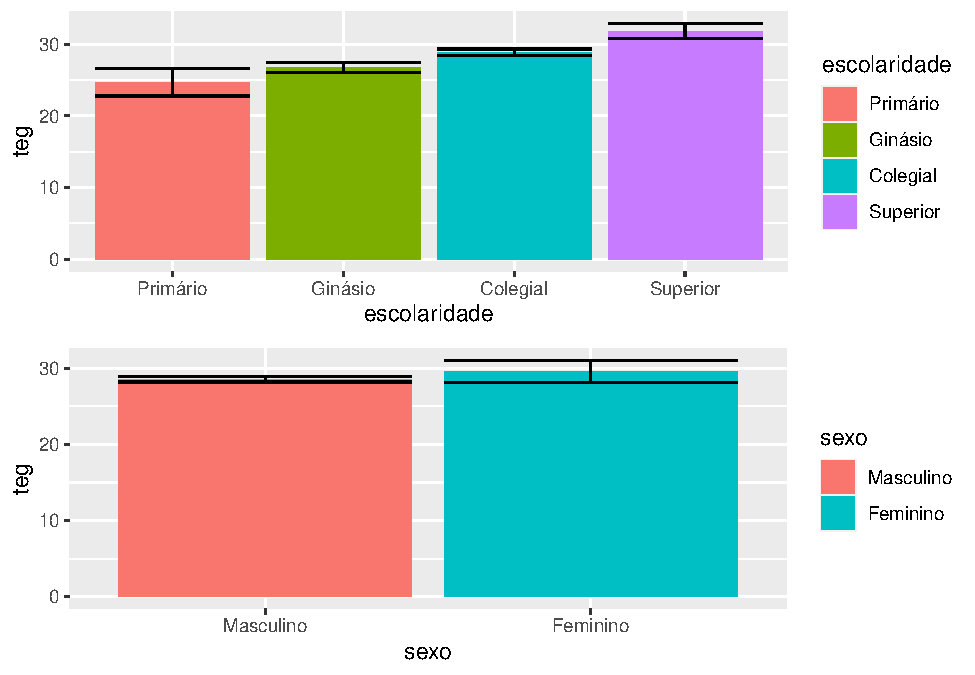
\includegraphics{gitbook-demo_files/figure-latex/unnamed-chunk-66-1} \end{center}

Agora, formalmente a modelagem será feita. Os passos devem ser exatamente os mesmos, incluindo a verificação de pressupostos e interpretação dos resultados. A esse momento, a tabela padronizada da ANOVA é a seguinte:

\begin{longtable}[]{@{}lllll@{}}
\toprule
Preditor & Soma dos Quadrados & Graus de liberdade & Quadrado médio & Estat. F\tabularnewline
\midrule
\endhead
Fator (A) & Entre (SS(A)) & K(A)-1 & MS(A) = SS(A)/k-1 & F = MS(A)/MSW\tabularnewline
Fator (B) & Entre (SS(B)) & K(B)-1 & MS(B) = SS(B)/k-1 & F = MS(B)/MSW\tabularnewline
Resíduo & Dentro (SSW) & N-1-(df(A)+df(B)) & MSW = SSW/N-1-(df(A)+df(B)) &\tabularnewline
\bottomrule
\end{longtable}

Posto isso, os resultados obtidos são:

\begin{Shaded}
\begin{Highlighting}[]
\NormalTok{mod_escolaridade_sexo <-}\StringTok{ }\KeywordTok{lm}\NormalTok{(teg }\OperatorTok{~}\StringTok{ }\NormalTok{escolaridade }\OperatorTok{+}\StringTok{ }\NormalTok{sexo, dados_teg)}
\NormalTok{apaTables}\OperatorTok{::}\KeywordTok{apa.aov.table}\NormalTok{(mod_escolaridade_sexo)}
\end{Highlighting}
\end{Shaded}

\begin{verbatim}
## 
## 
## ANOVA results using teg as the dependent variable
##  
## 
##     Predictor      SS  df      MS      F    p partial_eta2 CI_90_partial_eta2
##   (Intercept) 3650.67   1 3650.67 200.36 .000                                
##  escolaridade  450.51   3  150.17   8.24 .000          .15         [.06, .22]
##          sexo   14.93   1   14.93   0.82 .367          .01         [.00, .04]
##         Error 2587.34 142   18.22                                            
## 
## Note: Values in square brackets indicate the bounds of the 90% confidence interval for partial eta-squared
\end{verbatim}

Os resultados continuam constantando o efeito da escolaridade (F(3, 142) = 8.24, p \textless{} 0.01, ηp2 = 0.15, 90\% CI {[}.06, .22{]}) no empreendedorismo, mas também concluiu que o efeito do sexo não é significativo (F(1, 142) = 0.816, p = 0.36, ηp2 = 0.01, 90\% CI {[}.00, .04{]}). É importante ter atenção à forma de reportar os resultados, uma vez que delineamentos de dois fatores quase sempre produz coeficientes são diferentes do delineamento anterior. A análise post hoc que seria feita agora seria a mesma feita anteriormente e, em função disso, será suprimida.

Uma sugestão de escrita desses resultados é a seguinte:

\begin{writing}
\textbf{Como escrever os resultados}

Os dados foram analisados a partir de uma ANOVA de duas vias
investigando o efeito da escolaridade e do sexo no empreendedorismo. Foi
possível concluir que a escolaridade é um fator significativo aos
resultados (F(3, 142) = 8.24, p \textless{} 0.01, ηp2 = 0.15, 90\% CI
{[}.06, .22{]}), mas que o sexo não é significativo nessa relação (F(1,
142) = 0.81, p = 0.36, ηp2 = 0.01, 90\% CI {[}.00, .04{]}).
\end{writing}

\hypertarget{anova-fatorial}{%
\section{ANOVA Fatorial}\label{anova-fatorial}}

A ideia da ANOVA fatorial é provavelmente uma das mais frequentes em perguntas de pesquisas, que consistem em tentar saber se os fatores tem alguma interação entre si. Nesse sentido, a modelagem envolve o cálculo de um terceiro parâmetro para investigar essa relação. Dessa maneira:

\[y_i = b_0 + b_1X{_1}_i + b_2X{_2}_i + b_3(X{_1}_i * X{_2}_i) + \epsilon_{i}\]

Os coeficientes \(b_1\) e \(b_2\) estimam os efeitos principais, enquanto o \(b_3\) estima o efeito da interação.

Dessa vez, é importante ressaltar alguns aspectos:

\begin{enumerate}
\def\labelenumi{\arabic{enumi}.}
\item
  Apesar de efeitos de interação poderem ser exploratórios, a ideia de adicioná-lo é fortemente relacionada à teoria. Ou seja, a modelagem é frequentemente confirmatória;
\item
  A análise gráfica que é especialmente útil a todas as análises é ainda mais necessária nessa técnica;
\item
  A interpretação dos resultados sempre começa pela interação. Caso ela seja significativa, não se interpreta os efeitos principais.
\end{enumerate}

Nessa pesquisa, tivemos o interesse em saber se o nível de empreendedorismo varia em função de uma interação entre \texttt{sexo} e \texttt{estado\ civil} (solteiro ou casado) dos participantes. Ou seja, se o nível de homens e mulheres variava em função deles(as) serem casados(as) ou não. Em áreas comportamentais, a interação entre o efeito estado civil e do sexo em características sociais é bastante estudado.

\hypertarget{execuuxe7uxe3o-no-r-3}{%
\subsection{Execução no R}\label{execuuxe7uxe3o-no-r-3}}

Como mencionado, é fundamental ajustar todas as características da base para que os resultados não sejam distorcidos em função de definições computacionais. Como nessa pesquisa, também permitimos que pessoas divorciadas e viuvas, uma opção para deixar as análises totalmente pareadas com a pergunta da pesquisa é criar uma base contendo apenas solteiros (originalmente codificados com 1) e casados (originalmente codificados como 2).

\begin{Shaded}
\begin{Highlighting}[]
\NormalTok{base_interacao <-}\StringTok{ }\NormalTok{dados_teg }\OperatorTok\StringTok{ }\KeywordTok{filter}\NormalTok{(estado_civil }\OperatorTok{==}\StringTok{ "1"} \OperatorTok{|}\StringTok{ }\NormalTok{estado_civil }\OperatorTok{==}\StringTok{ "2"}\NormalTok{)}
\NormalTok{base_interacao <-}\StringTok{ }\NormalTok{base_interacao }\OperatorTok\StringTok{ }
\StringTok{  }\KeywordTok{mutate_at}\NormalTok{(}\KeywordTok{vars}\NormalTok{(estado_civil), }
    \OperatorTok{~}\KeywordTok{factor}\NormalTok{(}\KeywordTok{case_when}\NormalTok{(}
\NormalTok{      . }\OperatorTok{==}\StringTok{ }\DecValTok{1} \OperatorTok{~}\StringTok{ "solteiro"}\NormalTok{,}
\NormalTok{      . }\OperatorTok{==}\StringTok{ }\DecValTok{2} \OperatorTok{~}\StringTok{ "casado"}\NormalTok{), }\DataTypeTok{levels=}\KeywordTok{c}\NormalTok{(}\StringTok{"solteiro"}\NormalTok{,}\StringTok{"casado"}\NormalTok{)))}
\end{Highlighting}
\end{Shaded}

Agora o gráfico apresentado deve combinar as duas variáveis independentes, uma no eixo de X e outro no agrupamento. A escolha de como apresentar estas variáveis não deve ser aleatória, mas ser atrelada à forma da pergunta de pesquisa. Se o interesse for responder ``Quanto o estado civil depende do sexo para gerar os resultados do TEG'' sugere que em X coloque-se a variável ``estado civíl'' e no agrupamento a variáel "sexo.

\begin{Shaded}
\begin{Highlighting}[]
\KeywordTok{ggplot}\NormalTok{(base_interacao, }\KeywordTok{aes}\NormalTok{(}\DataTypeTok{x =}\NormalTok{ estado_civil, }\DataTypeTok{y =}\NormalTok{ teg, }\DataTypeTok{group =}\NormalTok{ sexo, }\DataTypeTok{col=}\NormalTok{ sexo)) }\OperatorTok{+}
\StringTok{  }\KeywordTok{geom_line}\NormalTok{(}\DataTypeTok{stat =} \StringTok{"summary"}\NormalTok{, }\DataTypeTok{size=}\DecValTok{1}\NormalTok{) }\OperatorTok{+}\StringTok{ }
\StringTok{  }\KeywordTok{stat_summary}\NormalTok{(}\DataTypeTok{fun.data =}\NormalTok{ mean_se, }\DataTypeTok{geom =} \StringTok{"errorbar"}\NormalTok{, }\DataTypeTok{width=}\FloatTok{0.1}\NormalTok{, }\DataTypeTok{size=}\DecValTok{1}\NormalTok{)}
\end{Highlighting}
\end{Shaded}

\begin{center}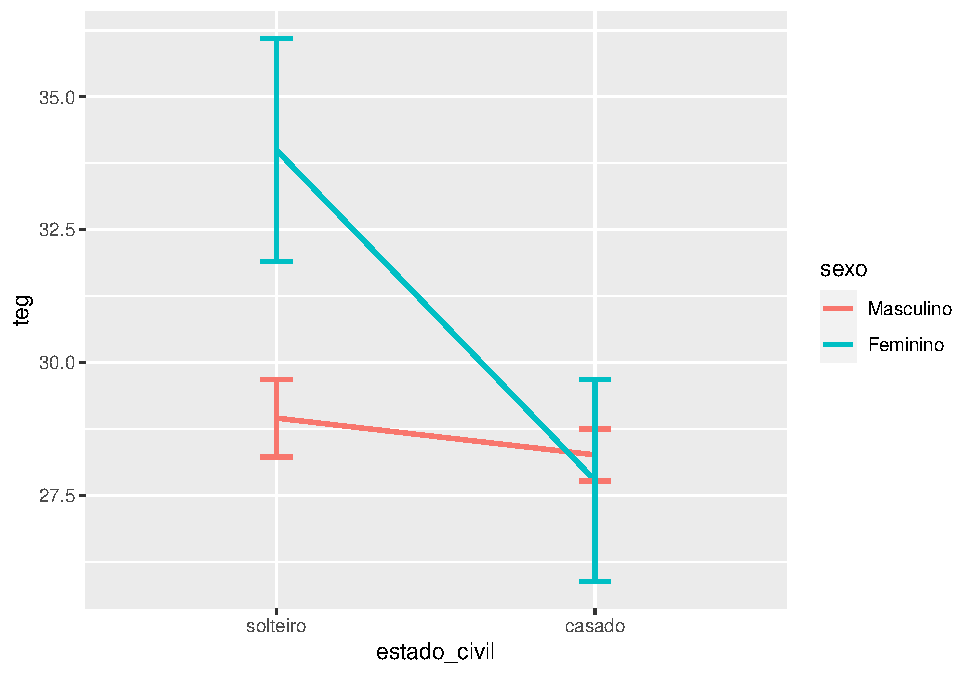
\includegraphics{gitbook-demo_files/figure-latex/unnamed-chunk-71-1} \end{center}

O gráfico indica que existe um efeito de interação, uma vez que as linhas se cruzam. No entanto, o teste formal deve ser feito. Da mesma forma do realizado anteriormente, a modelagem omitirá a verificação dos pressupostos, que foi apresentada em etapa inicial.

\begin{Shaded}
\begin{Highlighting}[]
\NormalTok{mod_int_sexo_civil <-}\StringTok{ }\KeywordTok{lm}\NormalTok{(teg }\OperatorTok{~}\StringTok{ }\NormalTok{sexo }\OperatorTok{*}\StringTok{ }\NormalTok{estado_civil, base_interacao)}
\NormalTok{apaTables}\OperatorTok{::}\KeywordTok{apa.aov.table}\NormalTok{(mod_int_sexo_civil)}
\end{Highlighting}
\end{Shaded}

\begin{verbatim}
## 
## 
## ANOVA results using teg as the dependent variable
##  
## 
##            Predictor       SS  df       MS       F    p partial_eta2
##          (Intercept) 35206.10   1 35206.10 1696.99 .000             
##                 sexo   113.84   1   113.84    5.49 .021          .04
##         estado_civil    13.04   1    13.04    0.63 .429          .00
##  sexo x estado_civil    87.89   1    87.89    4.24 .042          .03
##                Error  2676.27 129    20.75                          
##  CI_90_partial_eta2
##                    
##          [.00, .11]
##          [.00, .04]
##          [.00, .10]
##                    
## 
## Note: Values in square brackets indicate the bounds of the 90% confidence interval for partial eta-squared
\end{verbatim}

A leitura da tabela começa de cima para baixo, ou seja, pela interação. Neses caso, ela é significativa (F1, 129) = 4.23, p \textless{} 0.05, ηp2 = 0.03, 90\% CI {[}.00, .10{]}). Quando isso acontece, não se deve interpretar os efeitos principais, mesmo que eles sejam significativos.

\hypertarget{post-hoc-1}{%
\subsection{Post hoc}\label{post-hoc-1}}

No caso, à pergunta ``o sexo tem efeito no empreendedorismo'', a resposta adequada seria ``depende'', uma vez que ele varia em função do estado civil do participante. O post hoc vez será também feito pelo pacote \texttt{emmeans}, que já foi carregado anteriormente. Para deixar a rotina clara, vamos armazenar os resultados no objeto \texttt{post\_hoc\_int} e, em seguida, explorar os coeficientes.Repare que dessa vez, os valores de p ajustados ou não são os mesmos, dado que há apenas duas categorias em cada grupo.

\begin{Shaded}
\begin{Highlighting}[]
\NormalTok{post_hoc_int <-}\StringTok{ }\KeywordTok{emmeans}\NormalTok{(mod_int_sexo_civil, pairwise }\OperatorTok{~}\StringTok{ }\NormalTok{sexo }\OperatorTok{*}\StringTok{ }\NormalTok{estado_civil, }\DataTypeTok{adjust =} \StringTok{"bonferroni"}\NormalTok{)}
\end{Highlighting}
\end{Shaded}

O resultado deve ser acessado via contrastes.

\begin{Shaded}
\begin{Highlighting}[]
\NormalTok{post_hoc_int}\OperatorTok{$}\NormalTok{contrasts }\OperatorTok\StringTok{ }
\StringTok{  }\KeywordTok{kable}\NormalTok{(}\DataTypeTok{digits =} \DecValTok{2}\NormalTok{) }\OperatorTok\StringTok{ }
\StringTok{  }\KeywordTok{kable_styling}\NormalTok{(}\DataTypeTok{bootstrap_options =} \KeywordTok{c}\NormalTok{(}\StringTok{"striped"}\NormalTok{, }\StringTok{"hover"}\NormalTok{, }\StringTok{"condensed"}\NormalTok{))}
\end{Highlighting}
\end{Shaded}

contrast

estimate

SE

df

t.ratio

p.value

Masculino,solteiro - Feminino,solteiro

-5.05

2.15

129

-2.34

0.12

Masculino,solteiro - Masculino,casado

0.69

0.87

129

0.79

1.00

Masculino,solteiro - Feminino,casado

1.17

1.67

129

0.70

1.00

Feminino,solteiro - Masculino,casado

5.74

2.10

129

2.73

0.04

Feminino,solteiro - Feminino,casado

6.22

2.54

129

2.45

0.09

Masculino,casado - Feminino,casado

0.48

1.60

129

0.30

1.00

Repare que as informações repetem aquilo já visualizado no gráfico anterior, mas com as correções, a interpretação torna-se menos visual. Os resultados indicam que as mulheres solteiras têm resultados mais elevados do que os homens casados (Δ = 5.74, p = 0.04) e que existe uma tendência das mulheres solteiras, quando comparadas às mulheres casadas, terem também mais empreendedorismo (Δ = 6.22, p = 0.09). Repare que a diferença visual entre homens e mulheres solteiras não é significativa. Em linhas gerais, parece que o empreendedorismo diminui em pessoas casadas e isso é especialmente válido às mulheres.

\hypertarget{resumo-2}{%
\section{Resumo}\label{resumo-2}}

Este capítulo apresentou a ANOVA tanto de uma forma bastante pragmática como de uma maneira mais conceitual e, consequentemente, complexa. De forma pragmática, ao classificar a ANOVA como um super teste T, é possível demonstrar a importância da correção do valor de P após múltiplas comparações. Sem esses ajustes, a chance de cometer falsos positivos aumentaria. Já em outro sentido, ao deixar claro que a ANOVA é um caso particular de modelos de regressão, é possível entender que ela é uma análise complexa e que se ajusta bem à grande parte das perguntas empíricas e teóricas realizadas em Psicologia e outras ciências comportamentais.

\hypertarget{regressuxe3o-linear-simples}{%
\chapter{Regressão linear simples}\label{regressuxe3o-linear-simples}}

Os modelos de regressão modelos estatísticos que relacionam o comportamento de uma variável resposta (Y) como uma função de variáveis condicionantes (X). Em larga escala, eles substituem os outros testes paramétricos vistos até agora. Assim, quase tudo o que foi visto durante os capítulos anteriormente são casos especiais de modelos de regressão. No entanto, é possível estudar tais modelos tanto de uma maneira operacional, com foco totalmente pragmático e aderente às recomendações tradicionais dos livros de estatística, ou de uma forma detalhada, em que ao estudar os modelos de regressão, quase que muitos conceitos da estatística inferencial e estatística matemática são revisitados.

Nesse capítulo, iremos ver ambas as maneiras, mas preservando o foco na capacidade operacional.

Conceitualmente, a regressão linear é apresentada como::

\[y_i = b_0 + b_1X{_1}_i + \epsilon_{i}\]

\(y_i\) representa a variável dependente\\
\(b_0\) é o intercepto (coeficiente linear)\\
\(b_1\) é a inclinação (coeficiente angular)\\
\(\epsilon_{i}\) é o erro/resíduo

\hypertarget{legenda-1}{%
\section{Legenda}\label{legenda-1}}

Diferentes termos são empregados em modelos de regressão A legenda a seguir visa auxiliar no entendimento de cada um deles e aproximar o leitor a conceitos amplos utilizados em modelos lineares:

\begin{writing}
\textbf{intercepto} (constante) - \(b_0\): Valor previsto de Y quando X
= 0\\
\textbf{Inclinação} (slope) - \(b_i \forall i \neq 0\): A diferença
média em unidades da variável dependente prevista em Y quando se altera
uma unidade de X.\\
\textbf{SSR}: Soma dos Quadrados da Regressão\\
\textbf{SSE}: Soma dos Quadrados dos Erros\\
\textbf{SST}: Soma dos Quadrados Total\\
\textbf{Variabilidade total} SST = SSR + SSE\\
\(R^2\) ou \textbf{Coeficiente de Determinação}: A porcentagem de
variação da variável dependente (Y) que pode ser atribuída à variabilida
da(s) variável (is) independente(s) (X)\\
\(R^2_{adj}\) ou \textbf{Coeficiente de Determinação ajustado}: Pondera
a porcentagem de variação da variável dependente (Y) que pode ser
atribuída à variabilida da(s) variável (is) independente(s) (X) pelo
número de variáveis explicativas e pelo número de observações da
amostra. É particularmente útil quando deseja-se comparar modelos de
regressão múltipla que prevêem a mesma variável dependente, pois
penaliza aquele modelo com maior número de variáveis independentes.\\
RMSEA (\(Res. St. Error\) ou Erro padrão dos resíduos): Desvio padrão
dos valores previstos da variável dependente ao redor da linha de
regressão estimada
\end{writing}

O conhecimento das fórmulas fechadas também auxilia no entendimento da modelagem.

\begin{writing}
Soma dos Quadrados da Regressão:
\(SSR = \sum_{i=1}^{n}(\hat{y} - \bar{y})^2\)

Soma dos Quadrados dos Erros: \(SSE = \sum_{i=1}^{n}(y_i - \hat{y})^2\)

Soma dos Quadrados Total: \(SST = \sum_{i=1}^{n}(y_i - \bar{y})^2\)

\textbf{Variabilidade total} \(SST = SSR + SSE\)

\(R^2\) ou \textbf{Coeficiente de Determinação}: \$ R\^{}2 =
\frac{SSR}{SST} = 1- \frac{SSE}{SST}\$

Erro quadrático médio (MSE):
\(SSE = \sum_{i=1}^{n}(y_i - \hat{y})^2 /N-K\)

\(R^2_{adj}\) ou \textbf{Coeficiente de Determinação ajustado}:
\(1-\frac{MSE}{MSR}\)

\(Res. St. Error = \sqrt\frac{SSE}{N-K}\): Erro padrão dos resíduos, se
refere ao desvio padrão dos valores previstos da variável dependente ao
redor da linha de regressão estimada
\end{writing}

É possível citar ao menos três formas de explicar modelos de regressão. Evidentemente, todas são interligadas, mas cada qual apresenta uma ênfase didática diferente. Nesse sentido, a forma mais ``conceitual'' conta com conjuntos para explicitar o tema, a forma ``correlacional'' parte de um gráfico de dispersão e a forma ``analítica'' traz conceitos matemático. A forma correlacional é a mais simples de todas e iniciará o capítulo. A forma correlacional e analítica serão vistas a partir da pesquisa realizada.

\hypertarget{explicauxe7uxe3o-conceitual}{%
\section{Explicação conceitual}\label{explicauxe7uxe3o-conceitual}}

Inicialmente, é necessário atentar que a \texttt{variável\ dependente\ (Y)} e a \texttt{variável\ independente\ (X)} podem ser vistas como conjuntos. No caso:


\includegraphics{./img/cap_reg_x_y.png}

Repare que ambas as variáveis estão afastadas e não há nenhuma relação entre elas. No entanto, o que frequentemente ocorre é que existe algum grau de relacionamento entre elas, tal como exposto abaixo:

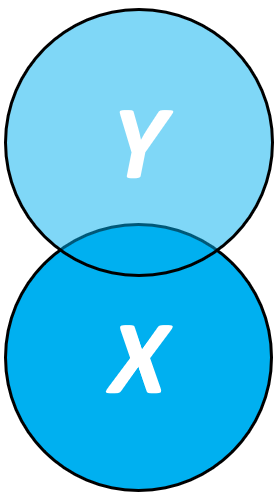
\includegraphics{./img/cap_reg_x_y2.png}

Nesse caso, vamos assumir que a variável X (independente) é um fator de causalidade à realização da variável dependente (Y). Em outras palavras, uma parte da realização de Y, necessariamente, depende de X. Essa área de interseção é entendida como a parte de Y que pode ser atribuída ou explicada por X. Analiticamente, essa área precisa de algumas transformações algébricas e, em função delas, recebe o nome de \texttt{Soma\ dos\ Quadrados\ da\ Regressão} (SSR, em inglês).

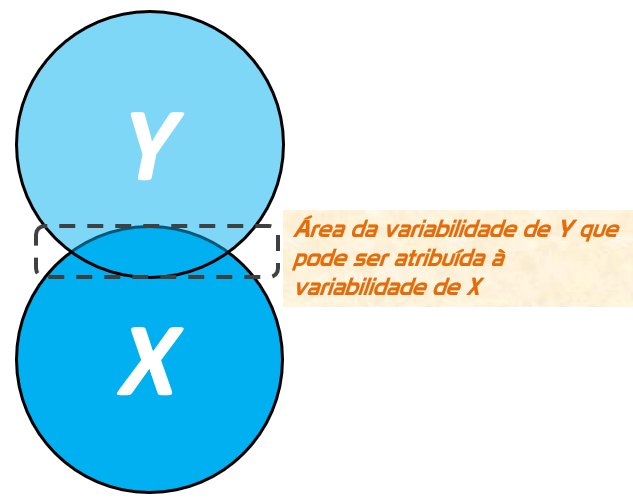
\includegraphics{./img/cap_reg_x_y_SSR.png}

No entanto, nem toda a variabilidade de Y pode ser atribuída à X. Essa região também sofrerá transformações algébricas e receberá o nome de \texttt{Soma\ dos\ Quadrados\ dos\ Erros} (SSE, em inglês). Essa área representa a variabilidade de Y que não pode ser atribuída/explicada por X. Nesse caso:

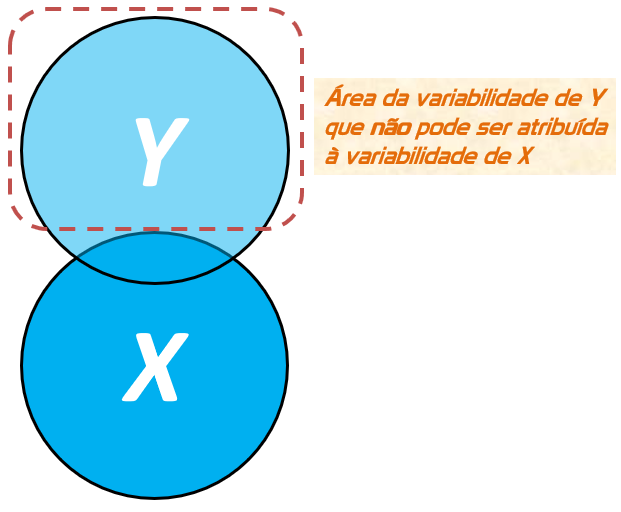
\includegraphics{./img/cap_reg_x_y_SSE.png}

É também possível verificar que a variável dependente (Y) têm uma variabilidade total, que também pode ser vista como o somatório da área explicada pela regressão (SSR-interseção) com a área não explicada (SSE). Essa região total também passará por transformações algébricas e receberá o nome de \texttt{Soma\ dos\ Quadrados\ Total} (SST, em inglês).

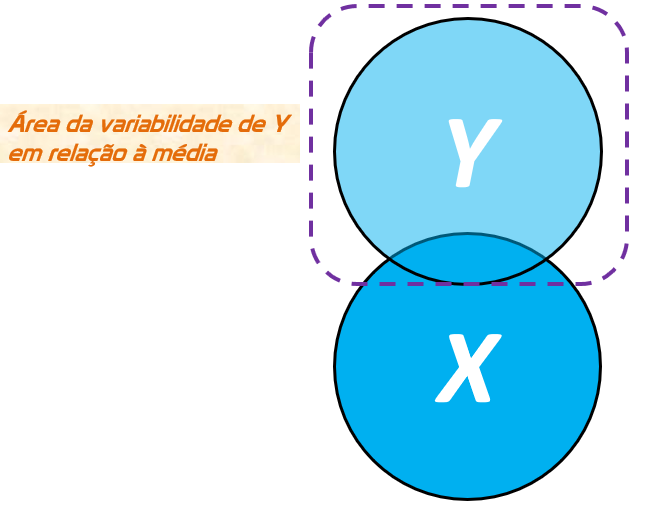
\includegraphics{./img/cap_reg_x_y_SST.png}

Vendo todas as partições de uma única vez, temos o seguinte:

\includegraphics{./img/cap_reg_x_y_SSR_SSE_SST.png}

Com isso, torna-se claro que a porcentagem de variação da variável dependente (Y) que pode ser atribuída à variabilidade de X é uma razão entre a Soma dos Quadrados da Regressão (SSR) pela Soma dos Quadrados Total (SST). O coeficiente obtido por essa razão recebe o nome de \textbf{Coeficiente de Determinação} ou \(R^2\).

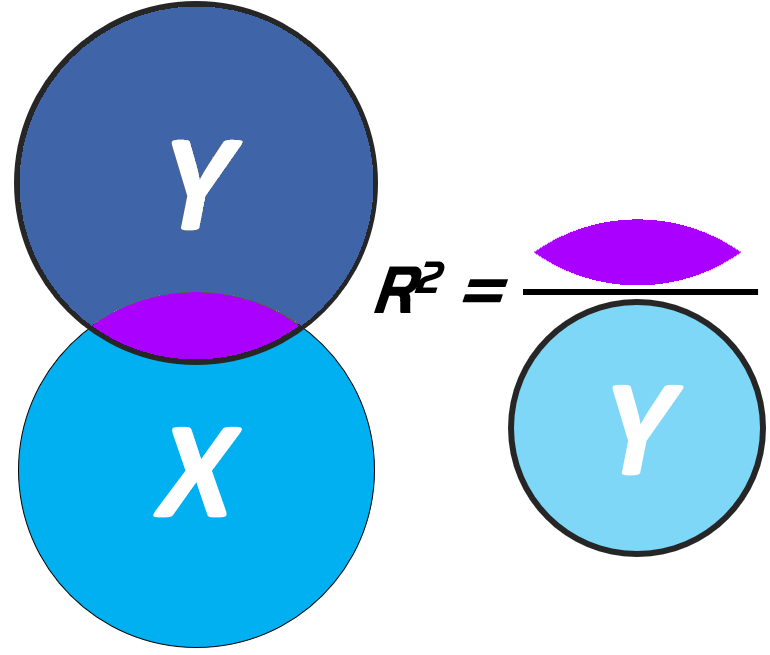
\includegraphics{./img/cap_reg_r2.png}

Isso é equivalente a subtração do espaço máximo de variabilidade (100\%) pela razão entre a Soma dos Quadrados dos Erros (SSE) pela Soma dos Quadrados Total (SST):

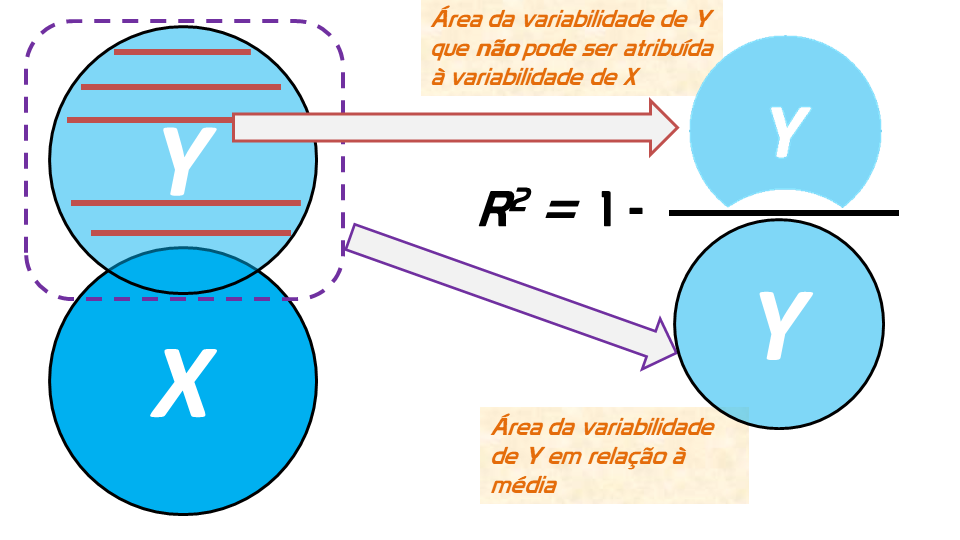
\includegraphics{./img/cap_reg_r2_1.png}

Evidentemente, modelos em que haja mais de uma variável independente (X) são frequentemente vistos por motivos óbvios. É muito improvável que uma única variável independente consiga explicar a variabilidade de variável dependente. Dessa maneira, é possível considerar Modelos de Regressão múltipla, tal como:

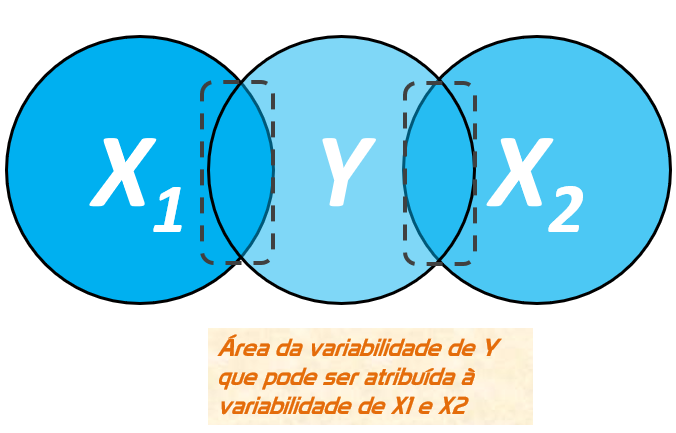
\includegraphics{./img/cap_reg_multipla_ortogonal.png}

Nesse modelo, há duas variáveis independentes (X1 e X2) e elas não tem nenhuma correlação \(\rho_{(X_1,X_2)}=0\)

A situação de correlação 0 entre X1 e X2 é muito improvavável. Modelos em que ambas as variáveis apresentam um grau de associação são frequentes:

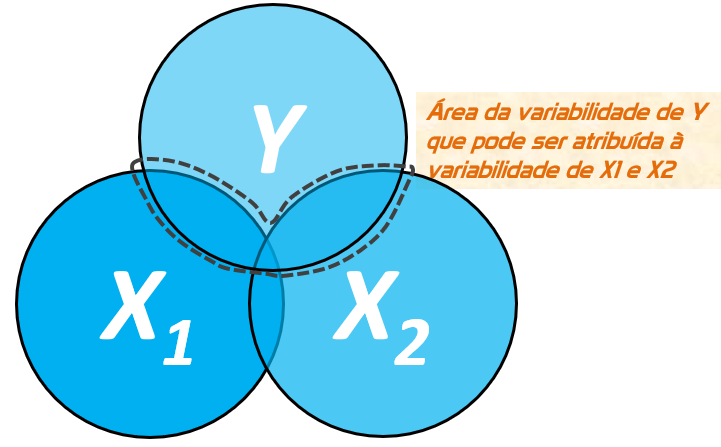
\includegraphics{./img/cap_reg_multipla.png}

A área em que existe uma interseção entre X1 e X2 chama-se de colinearidade. Caso haja mais de 2 variáveis também associadas, o nome é multicolinearidade.

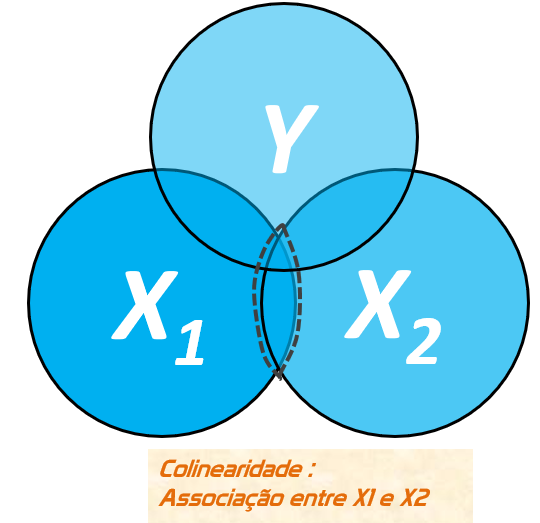
\includegraphics{./img/cap_reg_multipla_colinearidade.png}

Modelos assim serão explicitados em momento posterior.

\hypertarget{pesquisa-3}{%
\section{Pesquisa}\label{pesquisa-3}}

\begin{alert}

Base: Livro - Dados - Eating disorders

\end{alert}

Vamos utilizar a pesquisa intitulada ``Aspects Related to Body Image and Eating Behaviors in Healthy Brazilian Undergraduate Students'', publicada em 2018 no Global Journal of Educational Studies, que sou co-autor.

O objetivo dessa pesquisa foi explorar os fatores envolvidos em transtornos alimentares e aspectos da percepção da imagem corporal, bem como verificar a capacidade que uma medida possuia em predizer os resultados de outra. Esse artigo contou com a utilização de escalas aplicadas em 219 participantes no Brasil. Para acessar aspectos relacionados aos Transtornos alimentares, a escala EAT-26 foi aplicada. Para verificar aspectos da imagem corporal, a escala BSQ-34 foi aplicada.

Segue abaixo uma tabela inicial com dados descritivos dos resultados.

\begin{Shaded}
\begin{Highlighting}[]
\NormalTok{dados_brasil }\OperatorTok\StringTok{ }
\StringTok{  }\KeywordTok{group_by}\NormalTok{(sexo) }\OperatorTok\StringTok{ }
\StringTok{  }\KeywordTok{summarise_at}\NormalTok{(}\KeywordTok{vars}\NormalTok{(eat_soma, bsq_soma, imc, faz_esporte, familia_esporte), }
               \KeywordTok{list}\NormalTok{(}\OperatorTok{~}\KeywordTok{mean}\NormalTok{(., }\DataTypeTok{na.rm =} \OtherTok{TRUE}\NormalTok{), }\OperatorTok{~}\KeywordTok{sd}\NormalTok{(., }\DataTypeTok{na.rm =} \OtherTok{TRUE}\NormalTok{))) }\OperatorTok\StringTok{ }
\StringTok{  }\KeywordTok{t}\NormalTok{() }\OperatorTok
\StringTok{  }\KeywordTok{kable}\NormalTok{(., }\DataTypeTok{digits =} \DecValTok{2}\NormalTok{,  }\DataTypeTok{booktabs =}\NormalTok{ T) }\OperatorTok
\StringTok{  }\KeywordTok{kable_styling}\NormalTok{(}\DataTypeTok{position =} \StringTok{"center"}\NormalTok{, }\DataTypeTok{full_width =}\NormalTok{ F, }\DataTypeTok{bootstrap_options =} \StringTok{"striped"}\NormalTok{)}
\end{Highlighting}
\end{Shaded}

sexo

Homens

Mulheres

eat\_soma\_mean

12.64516

18.47619

bsq\_soma\_mean

64.23656

94.26190

imc\_mean

24.09761

22.58287

faz\_esporte\_mean

0.3978495

0.4523810

familia\_esporte\_mean

0.4782609

0.4761905

eat\_soma\_sd

8.188865

10.088976

bsq\_soma\_sd

32.86679

34.86458

imc\_sd

3.990227

3.150678

faz\_esporte\_sd

0.4921069

0.4997142

familia\_esporte\_sd

0.5022643

0.5014265

\hypertarget{regressuxe3o-linear-simples-1}{%
\section{Regressão linear simples}\label{regressuxe3o-linear-simples-1}}

A Regressão linear é uma técnica estatística utilizada que além de verificar o relacionamento funcional entre duas variáveis, permite criar uma equação que verifique o quanto os valores de uma variável varie em função de outra.

Há, ao menos, duas utilidades diretas em uma pesquisa, que são:

\begin{enumerate}
\def\labelenumi{(\roman{enumi})}
\item
  Predizer os valores da variável dependente (Y) em função dos valores da variável dependente (X);
\item
  Explicar a variabilidade da variável dependente (Y) em função da variável independente (X).
\end{enumerate}

Tecnicamente, ambas as utilidades são virtualmente iguais e como a Regressão linear simples pode ser vista a partir de um incremento ou avanço dos modelos de correlação, os aspectos correlacionais devem (e podem) ser inicialmente investigados.

\hypertarget{execuuxe7uxe3o-no-r-4}{%
\subsection{Execução no R}\label{execuuxe7uxe3o-no-r-4}}

Conforme já exposto, o gráfico de dispersão auxilia na visualização da relação entre as variáveis.A correlação entre ambas as medidas expressa a força e a direção que elas possuem. Enquanto a força é interpretada em \texttt{fraca} (0.1), \texttt{moderada} (0.3) ou \texttt{forte} (0.5), a direção pode ser positiva ou negativa, a depender do sinal.

\begin{Shaded}
\begin{Highlighting}[]
\KeywordTok{ggplot}\NormalTok{(dados_brasil, }\KeywordTok{aes}\NormalTok{(}\DataTypeTok{x =}\NormalTok{ bsq_soma, }\DataTypeTok{y =}\NormalTok{ eat_soma)) }\OperatorTok{+}
\StringTok{  }\KeywordTok{geom_jitter}\NormalTok{() }\OperatorTok{+}
\StringTok{  }\KeywordTok{labs}\NormalTok{(}\DataTypeTok{x =} \StringTok{"Resultados da Escala BSQ-34"}\NormalTok{, }\DataTypeTok{y =} \StringTok{"Resultados da Escala EAT-26"}\NormalTok{, }
       \DataTypeTok{title =} \StringTok{"Correlação entre o BSQ-34 e o EAT-26"}\NormalTok{)}
\end{Highlighting}
\end{Shaded}

\begin{center}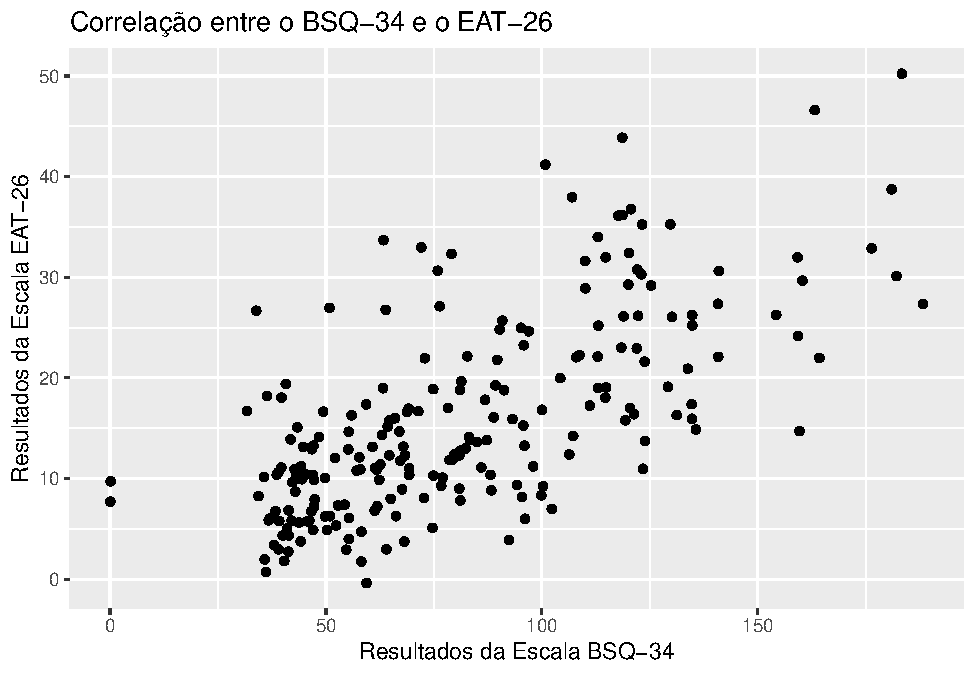
\includegraphics{gitbook-demo_files/figure-latex/unnamed-chunk-79-1} \end{center}

Tecnicamente, a correlação (de Pearson) nada mais é do que a padronização da covariância. Dessa forma,

\begin{Shaded}
\begin{Highlighting}[]
\NormalTok{(}\KeywordTok{cov}\NormalTok{(dados_brasil}\OperatorTok{$}\NormalTok{eat_soma, dados_brasil}\OperatorTok{$}\NormalTok{bsq_soma))}\OperatorTok{/}\NormalTok{(}\KeywordTok{sd}\NormalTok{(dados_brasil}\OperatorTok{$}\NormalTok{bsq_soma)}\OperatorTok{*}\KeywordTok{sd}\NormalTok{(dados_brasil}\OperatorTok{$}\NormalTok{eat_soma))}
\end{Highlighting}
\end{Shaded}

\begin{verbatim}
## [1] 0.6741895
\end{verbatim}

\[r(x,y) = \frac{COV(x,y)}{S(x)*S(y)} = \frac{243.6009}{361.3241} \approx 0.67\]

É necessário testar a hipótese que essa correlação poderia ser 0. A estatística do teste de significância da correlação segue uma distribuição T (n-2) graus de liberdade. Assim:

\[H_{0}: \rho = 0 \\ H_{a}: \rho \neq 0 \\ \alpha = 0.05\]

\[t = \frac{r_{xy}}{\sqrt\frac{1-r^2}{n-2}} = \frac{0.67}{\sqrt\frac{1-0.67^2}{219-2}} = 13.45\]

A comparação do valor calculado com o valor crítico (1.9709563) aponta que a \(H_0\) deve ser rejeitada. Assim, conclui-se que a correlação entre os resultados obtidos pelo \texttt{BSQ-34} e o \texttt{EAT-26} é significativa.

No entanto, é natural que o interesse de pesquisa seja verificar o quanto os resultados do \texttt{EAT-26} variam em função do \texttt{BSQ-34}, uma vez que alguns achados da literatura comentam que a alterações da alimentação ocorre em função da percepção da imagem corporal. Refraseando um pouco essa pergunta, o interesse agora é prever os valores do \texttt{EAT-26} a partir dos valores do \texttt{BSQ-34}. Como antes afirmado, esse objetivo é virtualmente identico a calcular o quanto a variabilidade dos resultados do \texttt{EAT-26} pode ser explicada pelos resultados do \texttt{BSQ-34}.

Fazer isso pede que se retorne ao gráfico correlacional feito ainda pouco e que tente se ajustar / traçar uma reta que tente tocar na maioria dos pontos. Milhões de retas podem ser traçadas e todas acertarão alguns pontos, mas errarão outros. Por exemplo

\begin{Shaded}
\begin{Highlighting}[]
\KeywordTok{ggplot}\NormalTok{(dados_brasil, }\KeywordTok{aes}\NormalTok{(}\DataTypeTok{x =}\NormalTok{ bsq_soma, }\DataTypeTok{y =}\NormalTok{ eat_soma)) }\OperatorTok{+}
\StringTok{  }\KeywordTok{geom_jitter}\NormalTok{() }\OperatorTok{+}
\StringTok{  }\KeywordTok{labs}\NormalTok{(}\DataTypeTok{x =} \StringTok{"Resultados da Escala BSQ-34"}\NormalTok{, }\DataTypeTok{y =} \StringTok{"Resultados da Escala EAT-26"}\NormalTok{, }
       \DataTypeTok{title =} \StringTok{"Correlação entre o BSQ-34 e o EAT-26"}\NormalTok{) }\OperatorTok{+}
\StringTok{  }\KeywordTok{geom_abline}\NormalTok{(}\DataTypeTok{slope =} \KeywordTok{c}\NormalTok{(}\KeywordTok{rnorm}\NormalTok{(}\DecValTok{10}\NormalTok{,}\FloatTok{0.4}\NormalTok{,}\FloatTok{0.5}\NormalTok{), }\KeywordTok{rnorm}\NormalTok{(}\DecValTok{10}\NormalTok{,}\FloatTok{0.2}\NormalTok{,}\FloatTok{0.2}\NormalTok{)),}\DataTypeTok{color =} \StringTok{"red"}\NormalTok{)}
\end{Highlighting}
\end{Shaded}

\begin{center}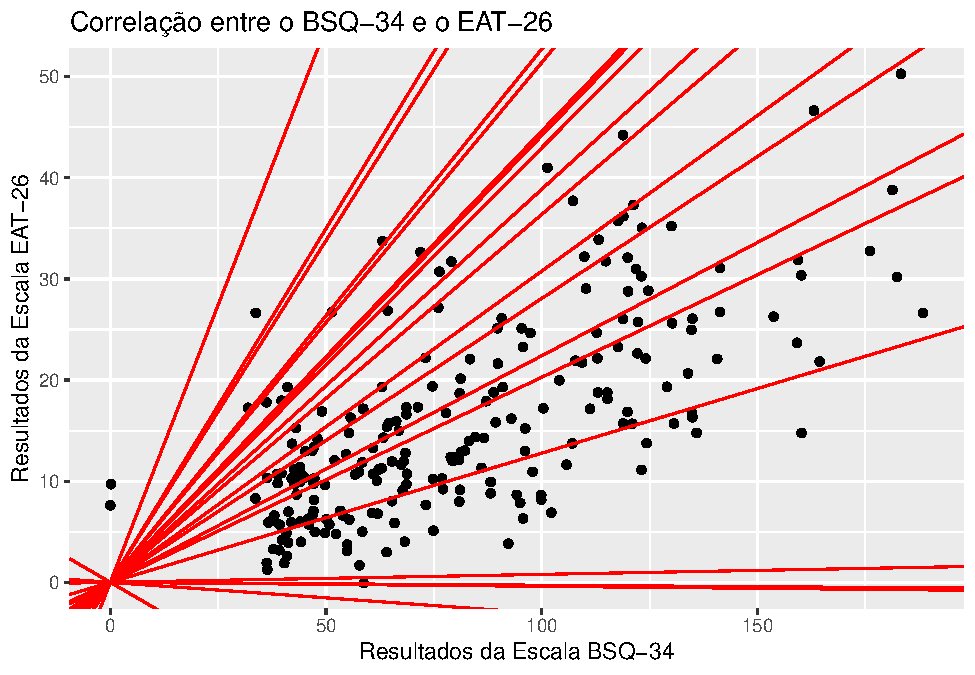
\includegraphics{gitbook-demo_files/figure-latex/unnamed-chunk-81-1} \end{center}

A necessidade agora é conseguir encontrar uma função que possa gerar uma reta que esteja bem perto dos pontos reais e, consequentemente, minimize os erros. Isso é feito justamente resgatando o conceito de função afim, exposto no ensino médio (e ilustrado ao início do capítulo)

\[\hat{y} = a + bx\]

Repare que agora o valor previsto (\(\hat{y}\)) depende de duas constantes (\texttt{a:\ intercepto\ ou\ coeficiente\ linear} e \texttt{b:\ inclinação\ ou\ coeficiente\ angular}) e uma variável (x). Apenas por uma questão de simbologia, três alterações são feitas com a equação:\\
(i) Os símbolos são alterados. Agora \(a = b_0\) e \(b = b_1\). A alteração de simbologia não altera em nada os cálculos.

\begin{enumerate}
\def\labelenumi{(\roman{enumi})}
\setcounter{enumi}{1}
\item
  Como se sabe que essa reta vai estimar os valores reais \(y\), letras minúsculas ou um chapéu sobre as letras será utilizado em vez das letras maiúsculas ou gregas.
\item
  Para que cada valor estimado seja associado a um participante a letra \(i\) será adicionada abaixo do \(y\), e do \(b_1\).\\
  Assim, temos que os valores estimados de y, agora \(\hat{y}\), são obtidos pelo \(b_0\) e \(b_1\):
\end{enumerate}

\[\hat{y}_i = b_0 + b_1X{_1}_i\]
No entanto, entre o valor real de y (os pontos que estão no gráfico) e os valores obtidos minha equação, haverá sempre uma certa quantidade de erro de estimativa (\(e_i\)). Ou seja, os valores estimados de cada participante (\(i\)) vão ter uma quantidade de erro (\(e_i\)). Dessa forma, é possível pensar que os valores reais agora possuem uma porção de erro:

\[y_i = a + b_1X{_1}_i+\underbrace{e_i}_\text{aleatório}\]

Do ponto de visto estatístico, é possível traçar milhões de retas, mas para encontrar a reta que minimize os erros, é necessário discriciona-lo.

\[e_i = y_i - \hat{y_i}\]
\[e_i = y_i - (b_0 + b_1X{_1}_i) \\ =  y_i - b_0 - b_1X{_1}_i\]

Quando se minimizar o erro (\(\epsilon_{i}\)), vai ser possível construir a reta mais próxima a todos os pontos. O método utilizado para isso é o Mínimos Quadrados Ordinários (em inglês, Ordinary Least Squares -- OLS), que visa minimizar a soma do quadrado dos resíduos. Para fazer isso, é necessário derivar os resíduos em relação a \(b_0\) e e \(b_1\) e igualar a 0:

\[\frac{\partial \epsilon}{\partial \beta_0}  = 0,\\ \frac{\partial \epsilon}{\partial \beta_1} = 0\]

E os resultados permitem concluir que:

\[\begin{aligned}
b_1 &= \frac{\sum_{i = 1}^{n} x_i y_i - \frac{(\sum_{i = 1}^{n} x_i)(\sum_{i = 1}^{n} y_i)}{n}}{\sum_{i = 1}^{n} x_i^2 - \frac{(\sum_{i = 1}^{n} x_i)^2}{n}} = \frac{COV(xy)}{VAR(x)}\\
b_0 &= \bar{y} - b_1 \bar{x}
\end{aligned}\]

Agora torna-se fácil traçar uma linha entre os pontos que minimize os erros. Uma vez que se sabe que:

\[b_1  = \frac{COV(xy)}{VAR(x)}\]
e que:

\[b_0  = \bar{y} - b_1\bar{x}\]

\begin{Shaded}
\begin{Highlighting}[]
\NormalTok{b1 <-}\StringTok{ }\KeywordTok{cov}\NormalTok{(dados_brasil}\OperatorTok{$}\NormalTok{bsq_soma, dados_brasil}\OperatorTok{$}\NormalTok{eat_soma)}\OperatorTok{/}\KeywordTok{var}\NormalTok{(dados_brasil}\OperatorTok{$}\NormalTok{bsq_soma)}
\NormalTok{b0 <-}\StringTok{ }\KeywordTok{mean}\NormalTok{(dados_brasil}\OperatorTok{$}\NormalTok{eat_soma)}\OperatorTok{-}\NormalTok{(b1}\OperatorTok{*}\KeywordTok{mean}\NormalTok{(dados_brasil}\OperatorTok{$}\NormalTok{bsq_soma))}

\KeywordTok{ggplot}\NormalTok{(dados_brasil, }\KeywordTok{aes}\NormalTok{(}\DataTypeTok{x =}\NormalTok{ bsq_soma, }\DataTypeTok{y =}\NormalTok{ eat_soma)) }\OperatorTok{+}
\StringTok{  }\KeywordTok{geom_jitter}\NormalTok{() }\OperatorTok{+}
\StringTok{  }\KeywordTok{labs}\NormalTok{(}\DataTypeTok{x =} \StringTok{"Resultados da Escala BSQ-34"}\NormalTok{, }\DataTypeTok{y =} \StringTok{"Resultados da Escala EAT-26"}\NormalTok{, }
       \DataTypeTok{title =} \StringTok{"Correlação entre o BSQ-34 e o EAT-26"}\NormalTok{) }\OperatorTok{+}
\StringTok{  }\KeywordTok{geom_abline}\NormalTok{(}\DataTypeTok{intercept =}\NormalTok{ b0, }\DataTypeTok{slope =}\NormalTok{ b1)}
\end{Highlighting}
\end{Shaded}

\begin{center}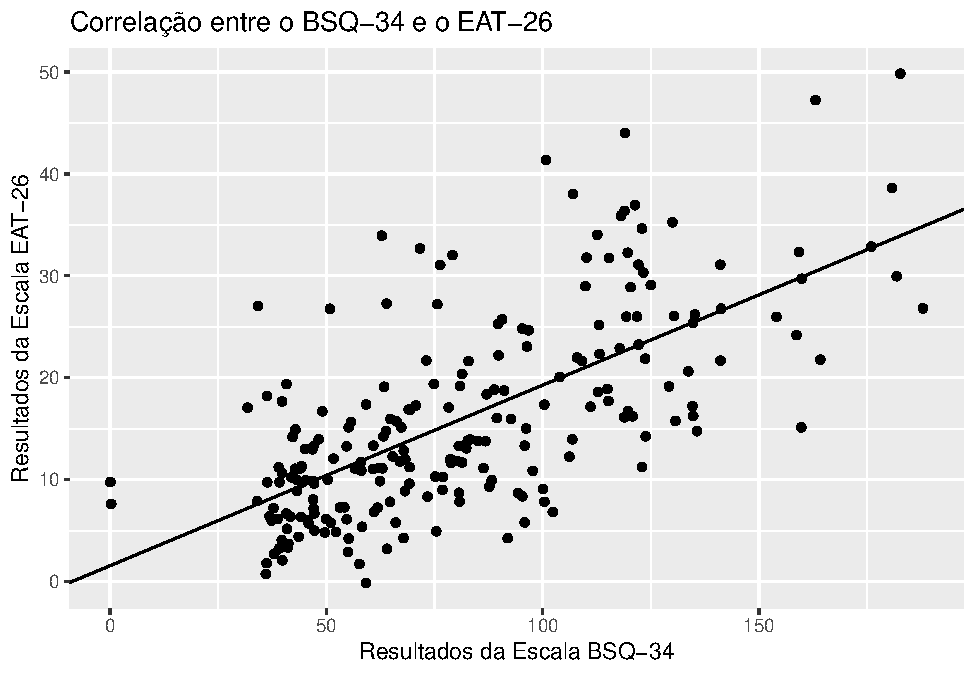
\includegraphics{gitbook-demo_files/figure-latex/unnamed-chunk-82-1} \end{center}

É também fácil notar que essa linha passará necessariamente pela média de ambas as variáveis.

\begin{Shaded}
\begin{Highlighting}[]
\KeywordTok{ggplot}\NormalTok{(dados_brasil, }\KeywordTok{aes}\NormalTok{(}\DataTypeTok{x =}\NormalTok{ bsq_soma, }\DataTypeTok{y =}\NormalTok{ eat_soma)) }\OperatorTok{+}
\StringTok{  }\KeywordTok{geom_jitter}\NormalTok{() }\OperatorTok{+}
\StringTok{  }\KeywordTok{labs}\NormalTok{(}\DataTypeTok{x =} \StringTok{"Resultados da Escala BSQ-34"}\NormalTok{, }\DataTypeTok{y =} \StringTok{"Resultados da Escala EAT-26"}\NormalTok{, }
       \DataTypeTok{title =} \StringTok{"Correlação entre o BSQ-34 e o EAT-26"}\NormalTok{) }\OperatorTok{+}
\StringTok{  }\KeywordTok{geom_abline}\NormalTok{(}\DataTypeTok{intercept =}\NormalTok{ b0, }\DataTypeTok{slope =}\NormalTok{ b1) }\OperatorTok{+}
\StringTok{  }\KeywordTok{geom_vline}\NormalTok{(}\DataTypeTok{xintercept =} \KeywordTok{mean}\NormalTok{(dados_brasil}\OperatorTok{$}\NormalTok{bsq_soma), }\DataTypeTok{size=}\FloatTok{1.5}\NormalTok{, }\DataTypeTok{color =} \StringTok{"red"}\NormalTok{, }\DataTypeTok{linetype =} \StringTok{"dashed"}\NormalTok{) }\OperatorTok{+}
\StringTok{  }\KeywordTok{geom_hline}\NormalTok{(}\DataTypeTok{yintercept =} \KeywordTok{mean}\NormalTok{(dados_brasil}\OperatorTok{$}\NormalTok{eat_soma), }\DataTypeTok{size=}\FloatTok{1.5}\NormalTok{, }\DataTypeTok{color =} \StringTok{"red"}\NormalTok{, }\DataTypeTok{linetype =} \StringTok{"dashed"}\NormalTok{)}
\end{Highlighting}
\end{Shaded}

\begin{center}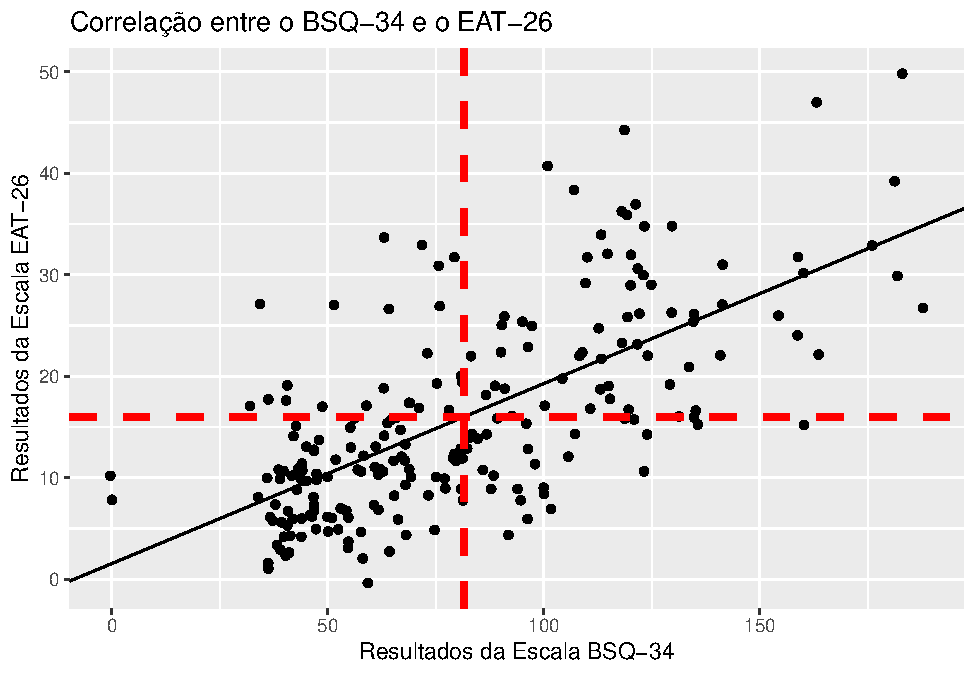
\includegraphics{gitbook-demo_files/figure-latex/unnamed-chunk-83-1} \end{center}

Ainda aproveitando o gráfico, agora torna-se mais simples de notar os dados reais, a linha de regressão e as distâncias (resíduos) entre os pontos reais e os previstos. Enquanto o modelo foi preciso em alguns pontos, em outros ele não se saiu assim tão bem. No entanto, como essa reta foi construída pela minimização da soma dos quadrados dos resíduos, isso nos deixa confortável com os resultados.

\begin{Shaded}
\begin{Highlighting}[]
\KeywordTok{transform}\NormalTok{(dados_brasil, }\DataTypeTok{Fitted =} \KeywordTok{fitted}\NormalTok{(mod_linear_simples)) }\OperatorTok\StringTok{ }
\StringTok{  }\KeywordTok{ggplot}\NormalTok{(., }\KeywordTok{aes}\NormalTok{(}\DataTypeTok{y =}\NormalTok{ bsq_soma, }\DataTypeTok{x =}\NormalTok{ eat_soma)) }\OperatorTok{+}
\StringTok{  }\KeywordTok{geom_point}\NormalTok{(}\KeywordTok{aes}\NormalTok{(}\DataTypeTok{y =}\NormalTok{ bsq_soma, }\DataTypeTok{x =}\NormalTok{ eat_soma, }\DataTypeTok{shape =} \StringTok{"real"}\NormalTok{), }\DataTypeTok{color=}\StringTok{"black"}\NormalTok{) }\OperatorTok{+}\StringTok{ }\CommentTok{#plot real}
\StringTok{  }\KeywordTok{geom_point}\NormalTok{(}\KeywordTok{aes}\NormalTok{(}\DataTypeTok{y =}\NormalTok{ Fitted, }\DataTypeTok{shape =}  \StringTok{"previsto"}\NormalTok{), }\DataTypeTok{color=}\StringTok{"1"}\NormalTok{) }\OperatorTok{+}\StringTok{ }\CommentTok{#plot previsto}
\StringTok{  }\KeywordTok{geom_smooth}\NormalTok{(}\DataTypeTok{se=}\OtherTok{FALSE}\NormalTok{, }\DataTypeTok{method =} \StringTok{"lm"}\NormalTok{, }\DataTypeTok{color =} \StringTok{"black"}\NormalTok{) }\OperatorTok{+}\StringTok{ }
\StringTok{  }\KeywordTok{geom_segment}\NormalTok{(}\KeywordTok{aes}\NormalTok{(}\DataTypeTok{x =}\NormalTok{ eat_soma, }\DataTypeTok{y =}\NormalTok{ bsq_soma, }\DataTypeTok{xend =}\NormalTok{ eat_soma, }\DataTypeTok{yend =}\NormalTok{ Fitted), }\DataTypeTok{color=} \StringTok{"red"}\NormalTok{) }\OperatorTok{+}\StringTok{ }\CommentTok{#erro ligado}
\StringTok{  }\KeywordTok{scale_colour_manual}\NormalTok{(}\DataTypeTok{name =} \StringTok{"Legenda"}\NormalTok{,}
                      \DataTypeTok{labels =} \KeywordTok{c}\NormalTok{(}\StringTok{"Estimados/Previstos"}\NormalTok{, }\StringTok{"Reais dos dados"}\NormalTok{),}
                      \DataTypeTok{values =} \KeywordTok{c}\NormalTok{(}\StringTok{"green"}\NormalTok{, }\StringTok{"black"}\NormalTok{)) }\OperatorTok{+}\StringTok{   }
\StringTok{  }\KeywordTok{scale_shape_manual}\NormalTok{(}\DataTypeTok{name =} \StringTok{"Legenda"}\NormalTok{,}
                     \DataTypeTok{labels =} \KeywordTok{c}\NormalTok{(}\StringTok{"Estimados/Previstos"}\NormalTok{, }\StringTok{"Reais dos dados"}\NormalTok{),}
                     \DataTypeTok{values =} \KeywordTok{c}\NormalTok{(}\DecValTok{1}\NormalTok{, }\DecValTok{5}\NormalTok{)) }\OperatorTok{+}
\StringTok{  }\KeywordTok{labs}\NormalTok{(}\DataTypeTok{x =} \StringTok{"Escala BSQ-34"}\NormalTok{, }\DataTypeTok{y =} \StringTok{"Escala EAT-26"}\NormalTok{, }\DataTypeTok{title =} \StringTok{"Resultados previstos vs. reais"}\NormalTok{)}
\end{Highlighting}
\end{Shaded}

\begin{verbatim}
## `geom_smooth()` using formula 'y ~ x'
\end{verbatim}

\begin{center}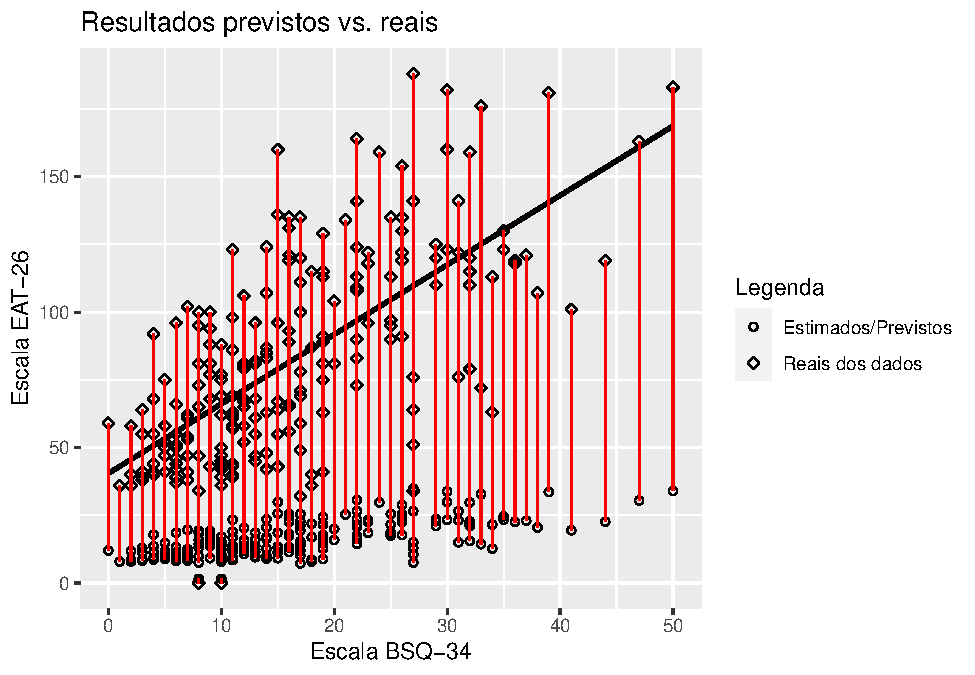
\includegraphics{gitbook-demo_files/figure-latex/unnamed-chunk-84-1} \end{center}

Posto isso, agora vamos, computacionalmente e analiticamente, realizar passo a passo a regressão linear simples. A função \texttt{lm} é a nativa para isso. Ela precisa da variável dependente e da variável independente, tal como abaixo.

\begin{Shaded}
\begin{Highlighting}[]
\NormalTok{mod_linear_simples <-}\StringTok{ }\KeywordTok{lm}\NormalTok{(eat_soma }\OperatorTok{~}\StringTok{ }\NormalTok{bsq_soma, }\DataTypeTok{data =}\NormalTok{ dados_brasil)}
\end{Highlighting}
\end{Shaded}

Existem diferentes maneiras de apresentar o resultado (que já calculamos inicialmente), A função \texttt{stargazer}, do pacote com mesmo nome, é uma das mais informativas e práticas. Assim:

\begin{Shaded}
\begin{Highlighting}[]
\KeywordTok{stargazer}\NormalTok{(mod_linear_simples, }\DataTypeTok{type =} \StringTok{'latex'}\NormalTok{) }
\end{Highlighting}
\end{Shaded}

\% Table created by stargazer v.5.2.2 by Marek Hlavac, Harvard University. E-mail: hlavac at fas.harvard.edu
\% Date and time: Sat, Jun 06, 2020 - 9:24:18 PM

\begin{table}[!htbp] \centering 
  \caption{} 
  \label{} 
\begin{tabular}{@{\extracolsep{5pt}}lc} 
\\[-1.8ex]\hline 
\hline \\[-1.8ex] 
 & \multicolumn{1}{c}{\textit{Dependent variable:}} \\ 
\cline{2-2} 
\\[-1.8ex] & eat\_soma \\ 
\hline \\[-1.8ex] 
 bsq\_soma & 0.177$^{***}$ \\ 
  & (0.013) \\ 
  & \\ 
 Constant & 1.550 \\ 
  & (1.180) \\ 
  & \\ 
\hline \\[-1.8ex] 
Observations & 219 \\ 
R$^{2}$ & 0.455 \\ 
Adjusted R$^{2}$ & 0.452 \\ 
Residual Std. Error & 7.215 (df = 217) \\ 
F Statistic & 180.823$^{***}$ (df = 1; 217) \\ 
\hline 
\hline \\[-1.8ex] 
\textit{Note:}  & \multicolumn{1}{r}{$^{*}$p$<$0.1; $^{**}$p$<$0.05; $^{***}$p$<$0.01} \\ 
\end{tabular} 
\end{table}

\begin{writing}
\textbf{Importante}

Apesar de todas as informações estarem presentes, os resultados não
poderiam ser apresentados pelo \texttt{kable()} de maneira adequada.
Assim, além do \texttt{stargazer}, como feito aqui, é possível contar
com a função \texttt{summ} do pacote \texttt{jtools}, ou com a função
\texttt{tab\_model} do \texttt{sjPlot}
\end{writing}

Os resultados do \texttt{intercepto} (\(b_0\)) e da \texttt{inclinação} \(b_1\) já foram analisados anteriormente, mas agora há 4 outros resultados que serão descritos. Em \textbf{primeiro momento}, é necessário verificar o ajuste do modelo e isso é feito pela linha \texttt{F-statistic}. Esse resultado pode ser obtido (I) comparando os resultados do modelo em questão com um modelo em que apenas o intercepto é utilizado para prever todos os valores ou (ii) verificando o quanto o modelo em questão consegue explicar da variabilidade dos dados. As duas formas serão vistas, a começar pela primeira.

Em termos técnicos, chama-se o modelo em questão de modelo \textbf{irrestrito} (ou \textbf{Aumentado}), uma vez que ele possui pelo menos um preditor além do intercepto. Por contraste, chama-se o modelo que tem apenas a média de \textbf{intercepto-apenas} (ou \textbf{Compacto}, ou \textbf{restrito} ou \textbf{nulo}). Algebricamente, temos o seguinte:

Modelo Compacto: \(y_i = b_0 + e_i\)\\
Modelo Aumentado: \(y_i = b_0 + b_1X_{1i} + e_i\)

Tanto o modelo compacto quanto o modelo aumentado geram uma quantidade de erro. A Soma dos Quadrados dos Erros (SSE) de ambos os modelos é a métrica utilizada para esse indicador. No R, é chamado de por Residual Sums-of-Squares (RSS).

Algebricamente, temos:

\[SSE =  \sum_{i=1}^{n}(y_i - \hat{y_i})^2\]

One:
\(y_i\) = Valor real obtido\\
\(\hat{y_i}\) = Valor previsto pelo modelo

Repare que a SSE é o denominador da variância. Quão maior o valor da SSE, pior é o modelo. No Modelo Compacto (intercepto-apenas), esse valor é de \ensuremath{2.9956072\times 10^{5}}. A conta é relativamente simples, tal como ilustrado abaixo.

\begin{Shaded}
\begin{Highlighting}[]
\NormalTok{mod_intercepto_apenas <-}\StringTok{ }\KeywordTok{lm}\NormalTok{(eat_soma }\OperatorTok{~}\StringTok{ }\DecValTok{1}\NormalTok{, }\DataTypeTok{data =}\NormalTok{ dados_brasil)}
\CommentTok{#SSE - Soma dos quadrados dos erros -- intercept-only}
\NormalTok{dados_brasil <-}\StringTok{ }\NormalTok{dados_brasil }\OperatorTok\StringTok{ }\CommentTok{#pegar a base}
\StringTok{  }\KeywordTok{mutate}\NormalTok{(}\DataTypeTok{erros_intercepto_apenas =} \KeywordTok{residuals}\NormalTok{(mod_intercepto_apenas)}\OperatorTok{^}\DecValTok{2}\NormalTok{) }\CommentTok{#criar o somatório dos resíduos}

\NormalTok{dados_brasil }\OperatorTok\StringTok{ }
\StringTok{  }\KeywordTok{summarise}\NormalTok{(}\KeywordTok{sum}\NormalTok{(erros_intercepto_apenas)) }\OperatorTok\StringTok{ }\KeywordTok{deframe}\NormalTok{() ->}\StringTok{ }\NormalTok{sse_intercepto_apenas}
\end{Highlighting}
\end{Shaded}

No Modelo Aumentado, o SSE é de 11297.74. Vale lembrar que a previsão dos valores de \(\hat{y_i}\) desse modelo conta com os resultados da variável \texttt{bsq\_soma}

\begin{Shaded}
\begin{Highlighting}[]
\CommentTok{#SSE - Soma dos quadrados dos residuos -- modelo irrestrito}
\NormalTok{dados_brasil <-}\StringTok{ }\NormalTok{dados_brasil }\OperatorTok\StringTok{ }
\StringTok{  }\KeywordTok{mutate}\NormalTok{(}\DataTypeTok{erros_linear_simples =} \KeywordTok{residuals}\NormalTok{(mod_linear_simples)}\OperatorTok{^}\DecValTok{2}\NormalTok{)}

\NormalTok{dados_brasil }\OperatorTok\StringTok{ }
\StringTok{  }\KeywordTok{summarise}\NormalTok{(}\KeywordTok{sum}\NormalTok{(erros_linear_simples)) }\OperatorTok\StringTok{ }\KeywordTok{deframe}\NormalTok{() ->}\StringTok{ }\NormalTok{sse_linear_simples}
\end{Highlighting}
\end{Shaded}

A comparação entre os modelos é feita pela capacidade de redução proporcional do erro (em ingles, Proportional Reduction in Erro ou PRE) que ocorre ao inserir o preditor. Formalmente, estamos diante de um teste de hipóteses que assume, inicialmente, que o valor de \(b_1\) poderia ser simplesmente 0. Ou seja:

\[H_0: b_1 = 0 \\  H_a: b_1 \neq 0 \\ \alpha = 0.05\]

Caso o preditor inserido seja ``útil'' ao modelo, os valores previstos (\(\hat{y}\)) serão mais próximos aos valores reais e, consequentemente, os erros serão menores. Assim, a razão abaixo apresenta o quanto o Modelo A diminui no erro da estimativa.

\(PRE = \frac{SSE(C)-SSE(A)}{SSR(C)}\)

Ou

\(PRE = 1-\frac{11297.74}{20712} = 0.4545318\)

Pela conta, O Modelo Aumentado possui cerca de 45\% menos erro do que o Modelo Compacto. No entanto, não dá para assumir a priori se esse valor é significativo ou não, uma vez que o Modelo Aumentado tem também mais preditores/parâmetros do que o Modelo Compacto. Dessa maneira, é necessário verificar estatísticamente se a adição feita pelo Modelo Aumentado é significativa. Isso é feito a partir de uma Distribuição F e é realizado da seguinte maneira:

\(F = \frac{PRE/(PA − PC)}{(1−PRE)/(n−PA)}\)

onde:
PRE = Proportional reduction in error\\
PA = Quantidade de parâmetros no Modelo A (no caso, 2: \(b_0\) e \(b_1{eatsoma}\))\\
PC = Quantidade de parâmetros no Modelo C (No caso, apenas 1: \(b_0\))\\
n = Quantidade de participantes (no caso, 219)

\(F = \frac{0.45/(2 − 1)}{(1−0.45)/(219−2)}\)

O valor encontrado (180.82) deve ser comparado com o valor crítico associado a um nível de significância específico, que possui distribuição F com PA − PC graus de liberdade no numerador e n−PA no denominador. Nesse caso, considerando 0.05 de significância, o valor crítico é 3.8846687, ou:

\(X \sim F_{0.05}(PA − PC,n−PA) \\X \sim F_{0.05}(df = 1, df = 217)\)

Como temos visto no decorrer dos capítulos, quão maior a estatística de teste, menor o valor de P. Nesse caso, como o valor calculado é maior do que o valor crítico, o valor de p é menor do que o nível de significância eleito (p =\ensuremath{2.1976832\times 10^{-30}}). Isso indica que o Modelo Aumentado significativamente reduz os erros quando comparado ao Modelo Compacto.

Graficamente, temos a seguinte situação:

\begin{Shaded}
\begin{Highlighting}[]
\KeywordTok{grid.arrange}\NormalTok{(}
  \KeywordTok{ggplot}\NormalTok{(}\KeywordTok{data.frame}\NormalTok{(}\DataTypeTok{x=}\KeywordTok{c}\NormalTok{(}\DecValTok{0}\NormalTok{,}\DecValTok{5}\NormalTok{)), }\KeywordTok{aes}\NormalTok{(}\DataTypeTok{x=}\NormalTok{x)) }\OperatorTok{+}
\StringTok{     }\KeywordTok{stat_function}\NormalTok{(}\DataTypeTok{fun=}\NormalTok{df, }\DataTypeTok{args=}\KeywordTok{list}\NormalTok{(}\DataTypeTok{df1=}\DecValTok{1}\NormalTok{, }\DataTypeTok{df2=}\DecValTok{217}\NormalTok{), }\DataTypeTok{colour=}\StringTok{"blue"}\NormalTok{, }\DataTypeTok{size=}\FloatTok{0.5}\NormalTok{) }\OperatorTok{+}
\StringTok{     }\KeywordTok{geom_vline}\NormalTok{(}\DataTypeTok{xintercept =} \KeywordTok{qf}\NormalTok{(}\DecValTok{1}\FloatTok{-0.05}\NormalTok{, }\DecValTok{1}\NormalTok{, }\DecValTok{217}\NormalTok{)) }\OperatorTok{+}
\StringTok{      }\KeywordTok{annotate}\NormalTok{(}\StringTok{"text"}\NormalTok{, }\DataTypeTok{x=}\DecValTok{4}\NormalTok{, }\DataTypeTok{y=}\FloatTok{1.4}\NormalTok{, }\DataTypeTok{label =} \StringTok{"Valor crítico"}\NormalTok{) }\OperatorTok{+}
\StringTok{     }\KeywordTok{ggtitle}\NormalTok{(}\StringTok{"F Distribution"}\NormalTok{),}
  
  \KeywordTok{ggplot}\NormalTok{(}\KeywordTok{data.frame}\NormalTok{(}\DataTypeTok{x=}\KeywordTok{c}\NormalTok{(}\DecValTok{0}\NormalTok{,}\DecValTok{5}\NormalTok{)), }\KeywordTok{aes}\NormalTok{(}\DataTypeTok{x=}\NormalTok{x)) }\OperatorTok{+}
\StringTok{     }\KeywordTok{stat_function}\NormalTok{(}\DataTypeTok{fun=}\NormalTok{df, }\DataTypeTok{args=}\KeywordTok{list}\NormalTok{(}\DataTypeTok{df1=}\DecValTok{1}\NormalTok{, }\DataTypeTok{df2=}\DecValTok{217}\NormalTok{), }\DataTypeTok{colour=}\StringTok{"blue"}\NormalTok{, }\DataTypeTok{size=}\FloatTok{0.5}\NormalTok{) }\OperatorTok{+}
\StringTok{     }\KeywordTok{geom_vline}\NormalTok{(}\DataTypeTok{xintercept =} \KeywordTok{qf}\NormalTok{(}\DecValTok{1}\FloatTok{-0.05}\NormalTok{, }\DecValTok{1}\NormalTok{, }\DecValTok{217}\NormalTok{)) }\OperatorTok{+}
\StringTok{     }\KeywordTok{geom_vline}\NormalTok{(}\DataTypeTok{xintercept =} \DecValTok{180}\NormalTok{) }\OperatorTok{+}
\StringTok{     }\KeywordTok{annotate}\NormalTok{(}\StringTok{"text"}\NormalTok{, }\DataTypeTok{x=}\DecValTok{170}\NormalTok{, }\DataTypeTok{y=}\FloatTok{1.4}\NormalTok{, }\DataTypeTok{label =} \StringTok{"Valor calculado"}\NormalTok{) }\OperatorTok{+}
\StringTok{     }\KeywordTok{ggtitle}\NormalTok{(}\StringTok{"F Distribution"}\NormalTok{))}
\end{Highlighting}
\end{Shaded}

\begin{center}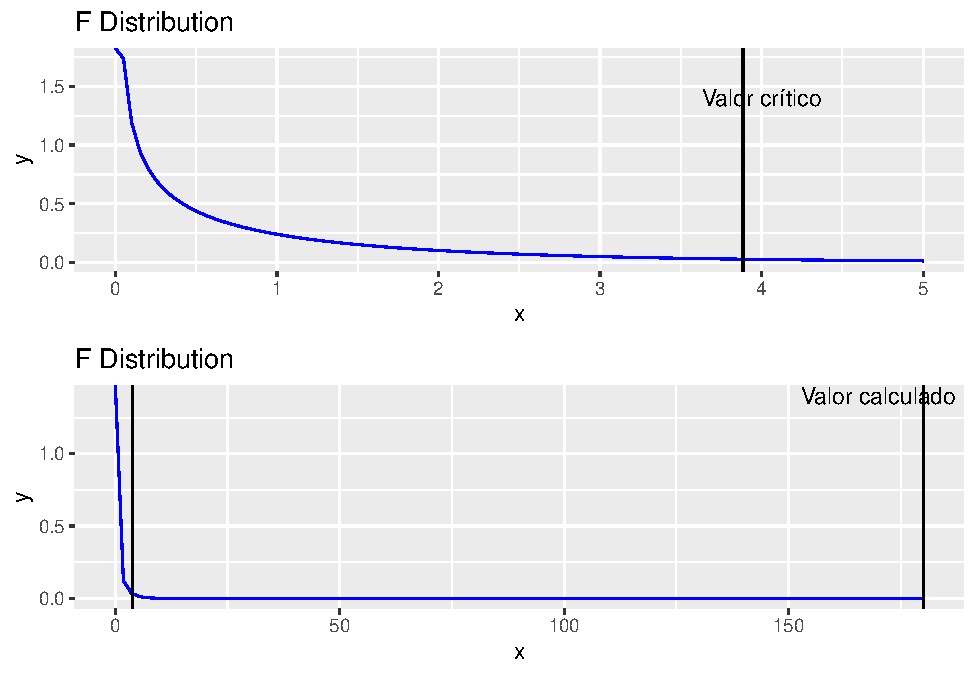
\includegraphics{gitbook-demo_files/figure-latex/unnamed-chunk-90-1} \end{center}

Agora, após esses cálculos, é possível concluir que a adição de um novo preditor no modelo reduz significativamente o erro presente em um modelo que conte apenas com a média (F(1, 217) = 180.8, p \textless{} 0.01). Posto isso, também é possível apresentar a função nativa \texttt{anova} que o R executa ao realizarmos a regressão. Repare que os valores encontrados são exatamente os mesmos (20712 para o SSE do Modelo Compacto e 11298 para o SSE do Modelo Aumentado). O valor de F também e p também são os mesmos (180.82 e p \textless{} 0,01).

\begin{Shaded}
\begin{Highlighting}[]
\KeywordTok{anova}\NormalTok{(mod_intercepto_apenas,mod_linear_simples)}
\end{Highlighting}
\end{Shaded}

\begin{verbatim}
## Analysis of Variance Table
## 
## Model 1: eat_soma ~ 1
## Model 2: eat_soma ~ bsq_soma
##   Res.Df   RSS Df Sum of Sq      F    Pr(>F)    
## 1    218 20712                                  
## 2    217 11298  1    9414.3 180.82 < 2.2e-16 ***
## ---
## Signif. codes:  0 '***' 0.001 '**' 0.01 '*' 0.05 '.' 0.1 ' ' 1
\end{verbatim}

No entanto, logo ao início comentamos que o \texttt{F-test} aponta para quanto o modelo em questão consegue explicar da variabilidade dos dados. Isso é feito pela razão entre a Regressão Quadrática Média (MSR) do Modelo Aumentado com o Erro Quadrático Médio (MSE) desse mesmo modelo.

\[ F = \frac{MSR}{MSE}\]

Da mesma maneira que foi explicado durante a ANOVA, o MSE é fruto da razão entre o SSR pelos graus de liberdade (K-1, considerando aqui o intercepto) e o MSR é fruto da razão entre o SSR pelos graus de liberdade (N-K, considerando também o intercepto). Nesse caso, o df do Modelo Aumentado é igual a 2 (\(b_0\) e \(b_1\)) e o df do resíduo é igual a 217 (219-2).

Abaixo a prova matemática:

\begin{Shaded}
\begin{Highlighting}[]
\NormalTok{dados_brasil }\OperatorTok\StringTok{ }
\StringTok{  }\KeywordTok{mutate}\NormalTok{(}\DataTypeTok{SSR_modelo_aumentado =}\NormalTok{ (}\KeywordTok{predict}\NormalTok{(mod_linear_simples)}\OperatorTok{-}\KeywordTok{mean}\NormalTok{(bsq_soma))}\OperatorTok{^}\DecValTok{2}\NormalTok{) }\OperatorTok\StringTok{ }
\StringTok{  }\KeywordTok{mutate}\NormalTok{(}\DataTypeTok{SSR_modelo_residuos =}\NormalTok{ (}\KeywordTok{predict}\NormalTok{(mod_linear_simples)}\OperatorTok{-}\NormalTok{bsq_soma)}\OperatorTok{^}\DecValTok{2}\NormalTok{) }\OperatorTok\StringTok{ }
\StringTok{  }\KeywordTok{summarise}\NormalTok{(}\DataTypeTok{F_statistic =}\NormalTok{ (}\KeywordTok{sum}\NormalTok{(SSR_modelo_aumentado)}\OperatorTok{/}\NormalTok{(}\DecValTok{2-1}\NormalTok{))}\OperatorTok{/}\NormalTok{(}\KeywordTok{sum}\NormalTok{(SSR_modelo_residuos)}\OperatorTok{/}\NormalTok{(}\KeywordTok{nrow}\NormalTok{(dados_brasil)}\OperatorTok{-}\DecValTok{2}\NormalTok{)))}
\end{Highlighting}
\end{Shaded}

\begin{verbatim}
## # A tibble: 1 x 1
##   F_statistic
##         <dbl>
## 1        180.
\end{verbatim}

Com isso posto, agora é possível montar a tabela inicial da regressão, que é exatamente igual ao que foi exposta no capítulo sobre a ANOVA (de uma via):

\begin{longtable}[]{@{}lllllll@{}}
\toprule
Source & SS & df & MS & F-Value & P-Value &\tabularnewline
\midrule
\endhead
Explicada & SSR (Regressão) & K-1 & MSR & SSR/K-1 & MSR/MSE & --\tabularnewline
Erro & SSE (Erro) & N-K & MSE & SSE/N-K & -- & --\tabularnewline
Total & SST (Total) & N-1 & var(y) & -- & -- & --\tabularnewline
\bottomrule
\end{longtable}

Com os valores reais, essa tabela fica:

\begin{longtable}[]{@{}llllll@{}}
\toprule
Source & SS & df & MSE & F-Value & P-Value\tabularnewline
\midrule
\endhead
Explicada & 9414.3 & 2-1 & 9414.3 & 180.823106 & --\tabularnewline
Resíduo & \ensuremath{1.12977\times 10^{4}} & 219-2 & 52.0633409 & -- & --\tabularnewline
Total & \ensuremath{2.0712\times 10^{4}} & 219-1 & -- & -- & --\tabularnewline
\bottomrule
\end{longtable}

Dito isso, o \textbf{segundo momento} é ainda calcado na análise dos resíduos. No caso, a raiz quadrada do erro quadratico médio indica o desvio padrão dos valores previstos da variável dependente ao redor da linha de regressão estimada. Algebricamente:

\[RMSE = \sqrt\frac{SSE}{N-K} = \sqrt{MSE}\]

No caso específico:

\[RMSE = \sqrt\frac{163401}{219-2} = 27.44\]

O \textbf{terceiro momento} se relaciona à interpretação do \(R^2\). Também chamado de \textbf{Coeficiente de Determinação}, ele mensura o quanto a variação total da variável dependente pode ser atribuída às variáveis independentes do modelo. Matematicamente, ele é equivalente ao PRE entre o Modelo Compacto e o Modelo Aumentado que, por sua vez, é equivalente à razão entre o SSR e a SST do Modelo Aumentado ou 1 - (SSE/SST)

Assim, o PRE era:

\(PRE = \frac{SSE(C)-SSE(A)}{SSR(C)}=\frac{299560.7-163401}{299560.7} = 0.4545318\)

Enquanto O R2 tem o mesmo valor:
\(R^2 = \frac{SSR}{SST} = \frac{136159.8}{299560.7} = 0.454\)\\
\(R^2 = 1-\frac{SSE}{SST} = 1- \frac{163401}{299560.7} = 0.454\)

Nesse caso, cerca de 45\% da variabilidade dos resultados da Escala EAT-26 podem ser atribuídos à variabilidade da Escala BSQ-34.

\begin{Shaded}
\begin{Highlighting}[]
\CommentTok{#Soma dos Quadrados Explicados - SSR}
\NormalTok{SSR_modelo_aumentado <-}\StringTok{ }\NormalTok{dados_brasil }\OperatorTok\StringTok{ }
\StringTok{  }\KeywordTok{mutate}\NormalTok{(}\DataTypeTok{SSR_modelo_aumentado =}\NormalTok{ (}\KeywordTok{predict}\NormalTok{(mod_linear_simples)}\OperatorTok{-}\KeywordTok{mean}\NormalTok{(eat_soma))}\OperatorTok{^}\DecValTok{2}\NormalTok{) }\OperatorTok
\StringTok{  }\KeywordTok{summarise}\NormalTok{(}\DataTypeTok{SSR_modelo_aumentado =}\NormalTok{ (}\KeywordTok{sum}\NormalTok{(SSR_modelo_aumentado))) }\OperatorTok\StringTok{ }
\StringTok{  }\KeywordTok{as.numeric}\NormalTok{() }\CommentTok{#9414.255}

\CommentTok{#Soma dos Quadrados dos erros - SSE}
\NormalTok{SSE_modelo_aumentado <-}\StringTok{ }\NormalTok{dados_brasil }\OperatorTok\StringTok{ }
\StringTok{  }\KeywordTok{mutate}\NormalTok{(}\DataTypeTok{SSE_modelo_aumentado =}\NormalTok{ (}\KeywordTok{predict}\NormalTok{(mod_linear_simples)}\OperatorTok{-}\NormalTok{eat_soma)}\OperatorTok{^}\DecValTok{2}\NormalTok{) }\OperatorTok
\StringTok{  }\KeywordTok{summarise}\NormalTok{(}\DataTypeTok{SSE_modelo_aumentado =}\NormalTok{ (}\KeywordTok{sum}\NormalTok{(SSE_modelo_aumentado))) }\OperatorTok\StringTok{ }
\StringTok{  }\KeywordTok{as.numeric}\NormalTok{() }\CommentTok{#11297.74}

\CommentTok{#Soma dos quadrados total - SST}
\NormalTok{sst_modelo_aumentado <-}\StringTok{ }\NormalTok{dados_brasil }\OperatorTok\StringTok{ }
\StringTok{  }\KeywordTok{mutate}\NormalTok{(}\DataTypeTok{sst_modelo_aumentado =}\NormalTok{ (eat_soma}\OperatorTok{-}\KeywordTok{mean}\NormalTok{(eat_soma))}\OperatorTok{^}\DecValTok{2}\NormalTok{) }\OperatorTok
\StringTok{  }\KeywordTok{summarise}\NormalTok{(}\DataTypeTok{sst_modelo_aumentado =}\NormalTok{ (}\KeywordTok{sum}\NormalTok{(sst_modelo_aumentado))) }\OperatorTok\StringTok{ }
\StringTok{  }\KeywordTok{as.numeric}\NormalTok{() }\CommentTok{#20712}
\end{Highlighting}
\end{Shaded}

Finalmente, o \textbf{quarto momento} é entender o \(R^2 ajustado\). Uma vez que modelos com mais parâmetros/preditores, independente da relevância deles, vão sempre ter \(R^2\) maior do que modelos mais compactos e, portanto, mais parcimoniosos, é necessário introduz uma punição ancorada na quantidade de preditores inseridos. Essa punição é realizada pelo \(R^2 ajustado\), que irá considerar a complexidade do modelo. Algebricamente é a mesma coisa que \(1-\frac{MSE}{MST} = 1-\frac{MSE}{VAR(Y)}\), como pode ser visto abaixo:

\[Adjusted R^2 = 1 - \frac{SSE/(N-K)}{SST/(N-1)} = 1-\frac{11297/217}{20712/218} = 1-\frac{52}{95} = 1 - 0.547 = 0.452\]

\begin{Shaded}
\begin{Highlighting}[]
\CommentTok{#variance }
\KeywordTok{sum}\NormalTok{((}\KeywordTok{mean}\NormalTok{(dados_brasil}\OperatorTok{$}\NormalTok{eat_soma)}\OperatorTok{-}\StringTok{ }\NormalTok{dados_brasil}\OperatorTok{$}\NormalTok{eat_soma)}\OperatorTok{^}\DecValTok{2}\NormalTok{)}\OperatorTok{/}\DecValTok{218}
\KeywordTok{var}\NormalTok{(dados_brasil}\OperatorTok{$}\NormalTok{eat_soma)}
\end{Highlighting}
\end{Shaded}

Com tais resultados descritos, agora é possível retornar aos coeficientes obtidos na regressão, que estão novamente listados abaixo.

\begin{Shaded}
\begin{Highlighting}[]
\KeywordTok{stargazer}\NormalTok{(mod_linear_simples, }\DataTypeTok{type =} \StringTok{"text"}\NormalTok{)}
\end{Highlighting}
\end{Shaded}

\begin{verbatim}
## 
## ===============================================
##                         Dependent variable:    
##                     ---------------------------
##                              eat_soma          
## -----------------------------------------------
## bsq_soma                     0.177***          
##                               (0.013)          
##                                                
## Constant                       1.550           
##                               (1.180)          
##                                                
## -----------------------------------------------
## Observations                    219            
## R2                             0.455           
## Adjusted R2                    0.452           
## Residual Std. Error      7.215 (df = 217)      
## F Statistic          180.823*** (df = 1; 217)  
## ===============================================
## Note:               *p<0.1; **p<0.05; ***p<0.01
\end{verbatim}

O \texttt{intercepto} é chamado de \texttt{constante} na maior parte dos programas e isso não é diferente no \texttt{stargazer}. No caso, ele se refere ao valor médio/esperado de Y quando X=0. Ou seja, se alguém tiveSSR tirado o valor 0 na escala BSQ-34, o valor previsto para os resultados da Escala EAT-26 seria de 1.55, tal como provado abaixo:

\begin{Shaded}
\begin{Highlighting}[]
\KeywordTok{predict}\NormalTok{(mod_linear_simples, }\KeywordTok{data.frame}\NormalTok{(}\DataTypeTok{bsq_soma=}\KeywordTok{c}\NormalTok{(}\DecValTok{0}\NormalTok{)))}
\end{Highlighting}
\end{Shaded}

\begin{verbatim}
##        1 
## 1.549962
\end{verbatim}

É importante notar que frequentemente o intercepto não tem interpretação lógica e, por isso, costuma ser desconsiderado. No entanto, é possível centralizar os valores do preditor \((x_i-\bar{x})\) para que o intercepto se torne o valor médio da variável dependente.

É também importante atentar que o valor do intercepto não é significativo, indicando que ele não é significativamente diferente de 0.

Já o coeficiente do \texttt{bsq\_soma}, que se refere os resultados obtidos a partir da Escala BSQ-34 é 0.177 e significativo. Isso significa que 1 unidade de mudança nos resultados da BSQ-34 geram 0.177 unidade de mudança, em média, nos resultados da Escala BSQ-34.

É importante atentar que o Erro Padrão (Std. Error) é justamente o que permite verificar a significância do resultado e segue uma T com n-2 graus de liberdade. Nesse caso, para o Intervalo de Confiança de \texttt{b1} é:

\[CI = b1 \pm t_{\alpha/2},_{n-2}*SE(b_1))
\\ b1 - SE(b_1) ≤ b1 ≤ b1 + SE(b_1)\]

\[CI = b1 \pm t_{\alpha/2},_{n-2}\sqrt{\dfrac{SSE/(N-k)}{\sum_{i=1}^{n}(x_i - \bar{x})^2}}\]

Torna-se claro, dessa forma, que a estatística T encontrada nada mais é do que:

\[T = \frac{b_1}{SE(b_1)} \\ T = \frac{2.5640}{0.1907} = 13.44\]

É importante atentar que na regressão linear simples, o intervalo de confiança de \(b_1\) é análogo à razão entre o RMSE por toda variação ao entorno de X

\[CI(b1)=\frac{RMSE}{\sqrt{n-1*S^2X}}\]

\begin{Shaded}
\begin{Highlighting}[]
\KeywordTok{sqrt}\NormalTok{(SSE_modelo_aumentado}\OperatorTok{/}\DecValTok{217}\NormalTok{)}

\NormalTok{(SSE_modelo_aumentado}\OperatorTok{/}\DecValTok{217}\NormalTok{)}\OperatorTok{*}\NormalTok{(}\DecValTok{1}\OperatorTok{/}\DecValTok{219}\NormalTok{)}\OperatorTok{+}\NormalTok{(}\KeywordTok{mean}\NormalTok{(dados_brasil}\OperatorTok{$}\NormalTok{bsq_soma)}\OperatorTok{^}\DecValTok{2}\NormalTok{)}\OperatorTok{/}\NormalTok{(}\KeywordTok{sum}\NormalTok{((}\KeywordTok{mean}\NormalTok{(dados_brasil}\OperatorTok{$}\NormalTok{bsq_soma)}\OperatorTok{-}\StringTok{ }\NormalTok{dados_brasil}\OperatorTok{$}\NormalTok{bsq_soma)}\OperatorTok{^}\DecValTok{2}\NormalTok{))}

\CommentTok{#Erro padrão do b0}
\KeywordTok{sqrt}\NormalTok{((SSE_modelo_aumentado}\OperatorTok{/}\DecValTok{217}\NormalTok{))}\OperatorTok{*}\KeywordTok{sqrt}\NormalTok{(((}\DecValTok{1}\OperatorTok{/}\DecValTok{219}\NormalTok{)}\OperatorTok{+}\NormalTok{(}\KeywordTok{mean}\NormalTok{(dados_brasil}\OperatorTok{$}\NormalTok{bsq_soma)}\OperatorTok{^}\DecValTok{2}\NormalTok{)}\OperatorTok{/}\NormalTok{(}\KeywordTok{sum}\NormalTok{((}\KeywordTok{mean}\NormalTok{(dados_brasil}\OperatorTok{$}\NormalTok{bsq_soma)}\OperatorTok{-}\StringTok{ }\NormalTok{dados_brasil}\OperatorTok{$}\NormalTok{bsq_soma)}\OperatorTok{^}\DecValTok{2}\NormalTok{))))}


\NormalTok{(SSE_modelo_aumentado}\OperatorTok{/}\DecValTok{217}\NormalTok{)}\OperatorTok{/}\KeywordTok{sqrt}\NormalTok{(((}\DecValTok{1}\OperatorTok{/}\DecValTok{219}\NormalTok{)}\OperatorTok{+}\NormalTok{(}\KeywordTok{mean}\NormalTok{(dados_brasil}\OperatorTok{$}\NormalTok{bsq_soma)}\OperatorTok{^}\DecValTok{2}\NormalTok{)}\OperatorTok{/}\NormalTok{(}\KeywordTok{sum}\NormalTok{((}\KeywordTok{mean}\NormalTok{(dados_brasil}\OperatorTok{$}\NormalTok{bsq_soma)}\OperatorTok{-}\StringTok{ }\NormalTok{dados_brasil}\OperatorTok{$}\NormalTok{bsq_soma)}\OperatorTok{^}\DecValTok{2}\NormalTok{))))}

\CommentTok{#https://www.ics.uci.edu/~sternh/courses/210/slides2new.pdf}
\end{Highlighting}
\end{Shaded}

Em relação ao \texttt{intercepto}, o intervalo de confiança também é baseado no erro padrão, tal como descrito abaixo:

\[CI = b0 \pm t_{\alpha/2},_{n-2}*SE(b_0))
\\ b0 - SE(b_0) ≤ b0 ≤ b0 + SE(b_0)\]

\[SS_{b0} = \sqrt{SSE/(N-K)(\frac{1}{n}+\frac{\bar{x}^2}{\sum_{i=1}^{n}(x_i - \bar{x})^2}})\]

A estatística de teste é dada pela razão entre a estimativa e o erro padrão.

\[ T = \frac{b0}{SE(b1)} \\ = \frac{0.177}{0.013} \\ \approx 13.4  \]

\hypertarget{pressupostos}{%
\section{Pressupostos}\label{pressupostos}}

\begin{Shaded}
\begin{Highlighting}[]
\KeywordTok{ggplot}\NormalTok{(dados_brasil, }\KeywordTok{aes}\NormalTok{(}\DataTypeTok{x =}\NormalTok{ bsq_media, }\DataTypeTok{y  =}\NormalTok{ bsq_soma)) }\OperatorTok{+}
\StringTok{  }\KeywordTok{geom_line}\NormalTok{()}
\end{Highlighting}
\end{Shaded}

\begin{center}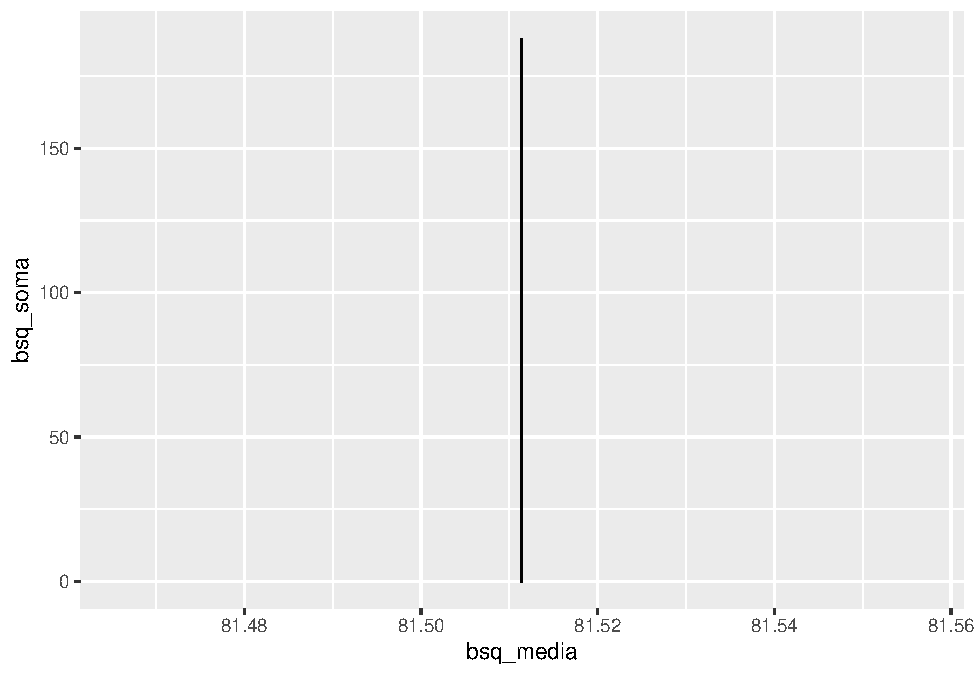
\includegraphics{gitbook-demo_files/figure-latex/unnamed-chunk-100-1} \end{center}

\begin{Shaded}
\begin{Highlighting}[]
\KeywordTok{cov}\NormalTok{(dados_brasil}\OperatorTok{$}\NormalTok{eat_soma,dados_brasil}\OperatorTok{$}\NormalTok{bsq_soma)}\OperatorTok{/}\KeywordTok{var}\NormalTok{(dados_brasil}\OperatorTok{$}\NormalTok{eat_soma)}
\end{Highlighting}
\end{Shaded}

\begin{verbatim}
## [1] 2.563973
\end{verbatim}

\begin{Shaded}
\begin{Highlighting}[]
\KeywordTok{mean}\NormalTok{(dados_brasil}\OperatorTok{$}\NormalTok{bsq_soma)}\OperatorTok{-}\KeywordTok{cov}\NormalTok{(dados_brasil}\OperatorTok{$}\NormalTok{eat_soma,dados_brasil}\OperatorTok{$}\NormalTok{bsq_soma)}\OperatorTok{/}\KeywordTok{var}\NormalTok{(dados_brasil}\OperatorTok{$}\NormalTok{eat_soma)}\OperatorTok{*}\KeywordTok{mean}\NormalTok{(dados_brasil}\OperatorTok{$}\NormalTok{eat_soma)}
\end{Highlighting}
\end{Shaded}

\begin{verbatim}
## [1] 40.48785
\end{verbatim}

Para utilizar os resultados, alguns pressupostos precisam ser atendidos. Tanto gráficos como testes formais podem ser utilizados para isso.

O primeiro é a linearidade.

\begin{Shaded}
\begin{Highlighting}[]
\KeywordTok{ggplot}\NormalTok{(dados_brasil, }\KeywordTok{aes}\NormalTok{(}\DataTypeTok{x =}\NormalTok{ eat_soma, }\DataTypeTok{y =}\NormalTok{ bsq_soma)) }\OperatorTok{+}
\StringTok{  }\KeywordTok{geom_jitter}\NormalTok{() }\OperatorTok{+}
\StringTok{  }\KeywordTok{geom_smooth}\NormalTok{(}\DataTypeTok{method =} \StringTok{"lm"}\NormalTok{)}
\end{Highlighting}
\end{Shaded}

\begin{verbatim}
## `geom_smooth()` using formula 'y ~ x'
\end{verbatim}

\begin{center}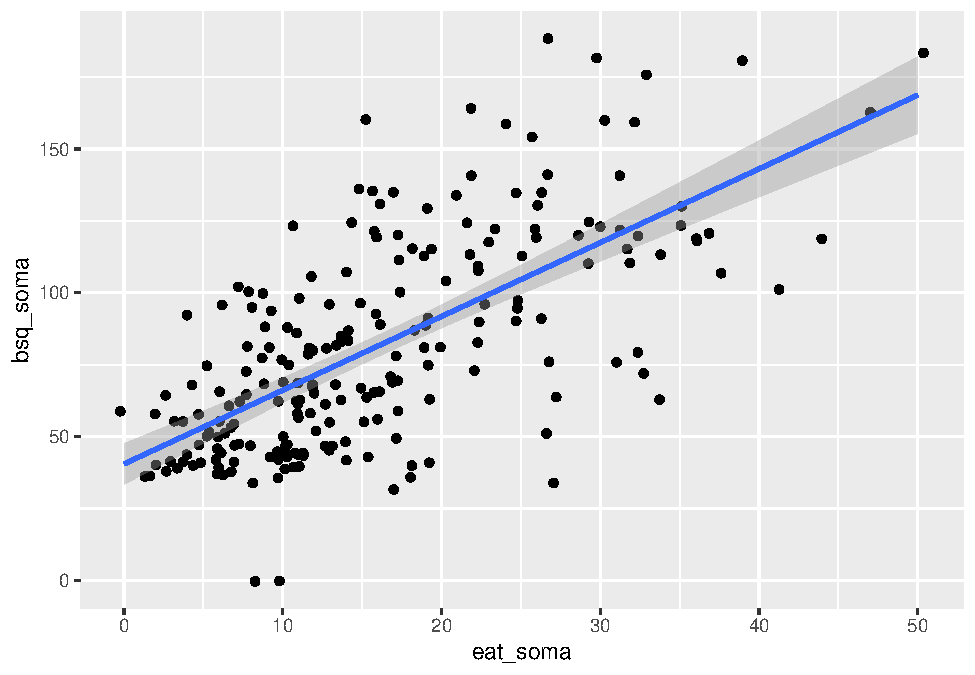
\includegraphics{gitbook-demo_files/figure-latex/unnamed-chunk-102-1} \end{center}

Em seguida, a independência dos resíduos, que pode ser calculada pela Variance inflation factors (VIF). Caso o valor do VIF supere 4, há sinal de multicolinearidade.

\(VIF = \frac{1}{1 - {R}^{2}_{k}} = \frac{1}{Tolerance}\)

\begin{Shaded}
\begin{Highlighting}[]
\KeywordTok{library}\NormalTok{(olsrr)}
\CommentTok{#ols_vif_tol(mod_linear_simples)}
\end{Highlighting}
\end{Shaded}

Os erros devem ser normalmentre distribuídos. Isso pode ser feito por um Q-Q plot. É indicado que não haja diferença entre a linha azul e a vermelha. Evidentemente, com dados empíricos (reais) isso é muito difícil.

\begin{Shaded}
\begin{Highlighting}[]
\KeywordTok{ols_plot_resid_qq}\NormalTok{(mod_linear_simples)}
\end{Highlighting}
\end{Shaded}

\begin{center}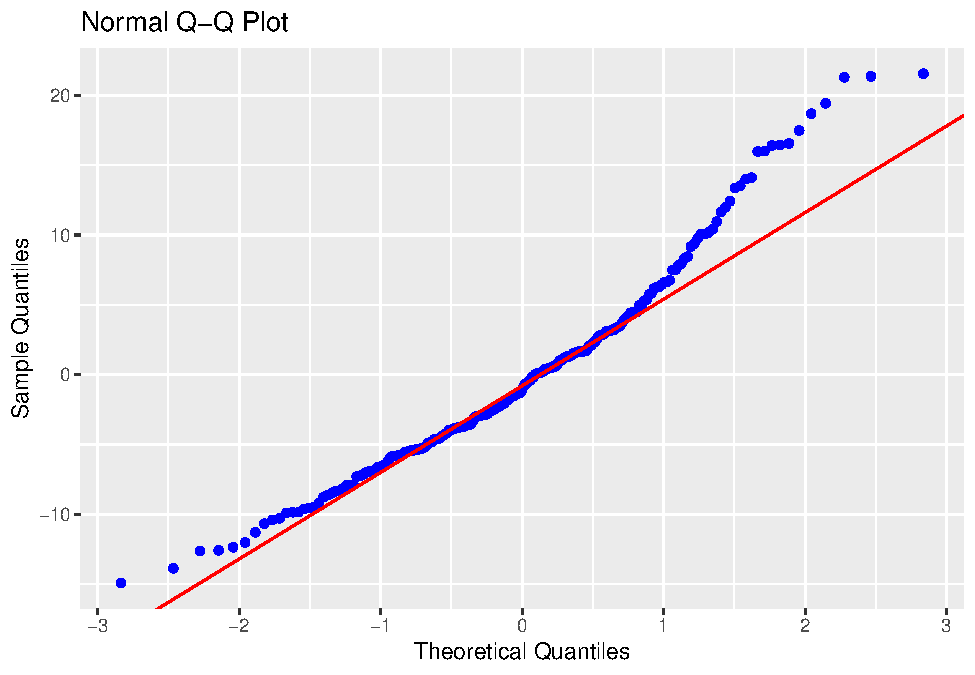
\includegraphics{gitbook-demo_files/figure-latex/unnamed-chunk-104-1} \end{center}

É também possível checar por um histograma, em que as barras devem ter similaridade à linha que apresenta a distribuição normal.

\begin{Shaded}
\begin{Highlighting}[]
\KeywordTok{ols_plot_resid_hist}\NormalTok{(mod_linear_simples)}
\end{Highlighting}
\end{Shaded}

\begin{center}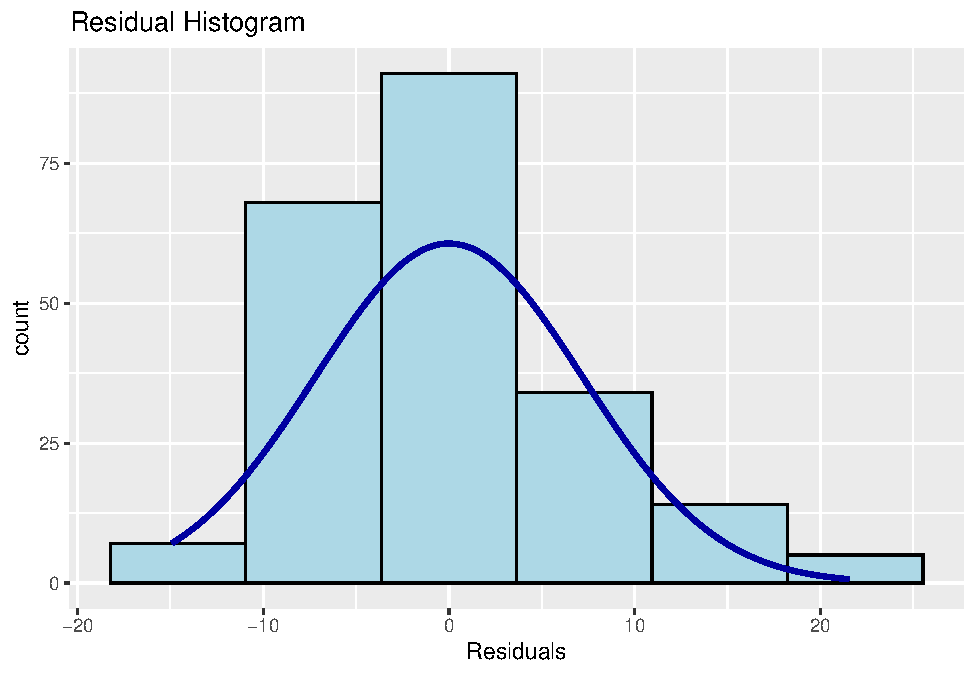
\includegraphics{gitbook-demo_files/figure-latex/unnamed-chunk-105-1} \end{center}

Os testes formaiss são o Shapiro-wilk, Kolgomorov-Smirnov, Cramer-von Mises e Anderson Darling. Em todos, a hipótese nula é de que os resíduos são normalmente distribuídos. Em função da modelagem matemática de cada um deSSRs testes, é esperado que eles tenham uma baixa performance em amostras menores que 30 e que os resultados entre eles sejam distintos quando a amostra é superior a 30, mas inferior a 200. A literatura tem mostrado que o Shapiro-Wilk é o teste com maior poder para detectar desvios da normalidade

\begin{Shaded}
\begin{Highlighting}[]
\KeywordTok{ols_test_normality}\NormalTok{(mod_linear_simples)}
\end{Highlighting}
\end{Shaded}

\begin{verbatim}
## Warning in ks.test(y, "pnorm", mean(y), sd(y)): ties should not be present for
## the Kolmogorov-Smirnov test
\end{verbatim}

\begin{verbatim}
## -----------------------------------------------
##        Test             Statistic       pvalue  
## -----------------------------------------------
## Shapiro-Wilk              0.9598         0.0000 
## Kolmogorov-Smirnov        0.0825         0.1017 
## Cramer-von Mises         16.9357         0.0000 
## Anderson-Darling          2.3975         0.0000 
## -----------------------------------------------
\end{verbatim}

De forma similar ao observado nos gráficos, os resultados majoritariamente apontam para normalidade dos resíduos.

As variâncias devem ser iguais (homocedasticidade). Iso pode ser visto em um gráfico de dispersão em que x é o valor previsto (fitted values) e y é o valor dos resíduos (residual). Traçar uma linha no centro de y facilita a visualização. O ideal é que padrões não sejam encontrados.

\begin{Shaded}
\begin{Highlighting}[]
\KeywordTok{include_graphics}\NormalTok{(}\StringTok{"img/cap_reg_homocedasticidade.png"}\NormalTok{)}
\end{Highlighting}
\end{Shaded}

\begin{center}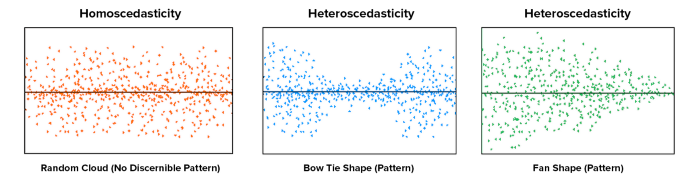
\includegraphics{img/cap_reg_homocedasticidade} \end{center}

\begin{Shaded}
\begin{Highlighting}[]
\KeywordTok{ols_plot_resid_fit}\NormalTok{(mod_linear_simples)}
\end{Highlighting}
\end{Shaded}

\begin{center}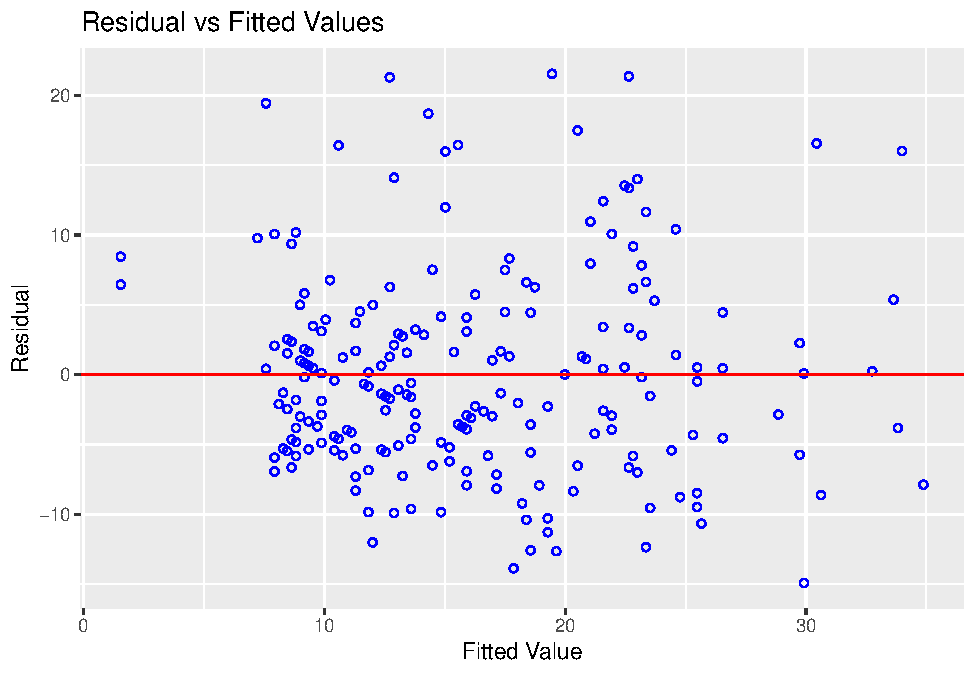
\includegraphics{gitbook-demo_files/figure-latex/unnamed-chunk-108-1} \end{center}

É possível visualizar que eSSR pressuposto é violado.

Exstem diferentes testes formais, como o Bartlett e o Breusch-Pagan. Os resultados costumam convergir e, em função da praticidade computacional, optaremos pelo teste de Breusch-Pagan. Nesseteste, os resultados tem distribuição qui-quadrado e a hipótese nula assume homocedasticidade. Portanto, a estatística de teste deveria ser insignificante para que a homocedasticidade pudeSSR ser aceita.

\begin{Shaded}
\begin{Highlighting}[]
\KeywordTok{ols_test_breusch_pagan}\NormalTok{(mod_linear_simples)}
\end{Highlighting}
\end{Shaded}

\begin{verbatim}
## 
##  Breusch Pagan Test for Heteroskedasticity
##  -----------------------------------------
##  Ho: the variance is constant            
##  Ha: the variance is not constant        
## 
##                 Data                 
##  ------------------------------------
##  Response : eat_soma 
##  Variables: fitted values of eat_soma 
## 
##         Test Summary          
##  -----------------------------
##  DF            =    1 
##  Chi2          =    8.980527 
##  Prob > Chi2   =    0.00272872
\end{verbatim}

\hypertarget{a-interpretauxe7uxe3o}{%
\section{A interpretação}\label{a-interpretauxe7uxe3o}}

Posto isso,

  \bibliography{book.bib,packages.bib}

\end{document}
